\documentclass[letter,12pt,dissertation]{OUdissertation6}
\usepackage{graphicx, subfigure} %allows .eps and .epsi graphics to be inserted
\usepackage{epic} %allows use of latex graphics
\usepackage{eepic} %allows use of latex graphics
\usepackage{amssymb,amsmath}
\usepackage{amsfonts}
\usepackage[amssymb]{SIunits}
\usepackage{multirow}
\usepackage{psfrag}
\usepackage{float}
\usepackage{bar}
\usepackage{rotating}
\let\autoref\ref


% Brian added this on July 15 2006 from suggestion of Di Jin:
\usepackage[centerfoot]{pageno}
\usepackage{natbib} %with amermeteorsoc.bst
%% For AMS,citations should be of the form ``author year''  not ``author, year'':
\bibpunct{(}{)}{;}{a}{}{,}

\newcommand{\be}{\begin{equation}} %these definitions save typing
\newcommand{\ee}{\end{equation}}
\newcommand{\bea}{\begin{eqnarray}}
\newcommand{\eea}{\end{eqnarray}}
\newcommand{\pd}[2]{\frac{\partial#1}{\partial#2}}
\newcommand{\pdd}[3]{\frac{\partial^{2}#1}{\partial#2 \partial#3}}
\newcommand{\bse}{\begin{subequations}}
\newcommand{\ese}{\end{subequations}}
\def\bal#1\eal{\begin{align}#1\end{align}}%allows for shortcut to align
\begin{document}
\title{DOWNSCALING TECHNIQUES FOR RETRIEVAL OF NEAR-SURFACE METEOROLOGICAL FIELDS AND TURBULENCE PARAMETERS FROM ATMOSPHERIC NUMERICAL MODEL OUTPUTS}
\author{JEREMY ALAN GIBBS}
\depositdate{2012}
\majorfield{SCHOOL OF METEOROLOGY}
\memberone{Prof. Evgeni Fedorovich}
\membertwo{Dr. Alexander van Eijk}
\memberthree{Prof. Lance Leslie}
%next two members are used in dissertation
\memberfour{Prof. Xuguang Wang}
\memberfive{Prof. Boris Apanasov}
%%%%
\begin{preface}
\prefacesectionX{Dedication}
Dedicate this to some people.

\prefacesectionX{Acknowledgements}
Acknowledge some people.
%must leave a blank line next to avoid bug:

\tableofcontents
\listoftables
\listoffigures
\prefacesection{Abstract}
The Weather Research and Forecasting (WRF) model has evolved toward a self- contained numerical weather prediction system, capable of modeling atmospheric motions ranging from global to microscales. The promise of such capability is appealing to both operational and research user communities for which accurate prediction of turbulence effects is increasingly desirable. Air pollution applications, for instance, rely on accurate representation of the dispersive role of small-scale atmospheric motions. On the other hand, many remote sensing applications depend on the accurate description of propagation of electromagnetic and acoustic waves in the turbulent atmosphere. The question of how best to adequately represent small-scale atmospheric motions in the range of scales of the order of 100 m and less based on numerical model output, remains a topic of debate.

Several methods have been evaluated in the reported study with a goal to identify an optimal approach to reproduce realistic near-surface flow fields and turbulence parameters using the mesoscale numerical model output. The focus of the study was primarily on the daytime flow fields corresponding to the convective boundary layer (CBL) conditions. A straightforward application of the WRF model in a traditional mesoscale configuration was the first evaluated approach. The WRF model applied in the large eddy simulation (LES) mode was another evaluated model configuration. This WRF-LES approach is not, however, without its share of performance concerns, particularly with respect to reproducibility of the smallest resolvable scales of motion. Approaches were also explored that are based on using the outputs of mesoscale models (including the WRF model) to nudge high-resolution LES of boundary-layer flows to realistic mesoscale environments. For this purpose, the OU-LES code was employed. Historically, this code has proven to be adequate for the reproduction of idealized CBL flows, but its technical implementation limits applicability to real-world situations.

Mean fields of meteorological quantities predicted by the WRF model in a mesoscale configuration generally compare favorably with observational and LES data. However, inspection of near-surface turbulence characteristics indicates that the model fails to adequately reproduce the spatial variability associated with atmospheric turbulence. Results from the WRF-LES indicate that the model tends to attribute more energy to larger-scale components of motion as compared to the conventional LES. Consequently, the WRF model fails to adequately reproduce spatial variability within sufficiently broad scale ranges. Spectra from the WRF model have narrower inertial subranges and point to over-dissipation on small scales of turbulent motion. Employment of the high-resolution OU-LES driven by the output of the WRF model run in the mesoscale-mode yielded the overall best results in terms of predicting near-surface turbulence parameters. This approach appears to be a best compromise in generating accurate bulk meteorological quantities and realistic turbulence statistics across a broad range of turbulence scales.
\end{preface}
\chapter{Introduction}
\label{intro-1}

\section{Motivation}
\label{motivation-11}

The trend in numerical weather prediction (NWP) is toward the use of fine grid meshes capable of resolving atmospheric motions down to the turbulence scale. The ability to reproduce credible small-scale spatial variability of meteorological fields is appealing to both operational and research environments. For instance, air pollution applications rely on accurate representation of the dispersive role of small-scale motions. Another example is the propagation of electromagnetic and acoustic waves in the atmosphere, for which structure-function parameters are highly dependent on atmospheric turbulence ~\citep{Wilson2012b}. Other areas in which such detail is critical include convective boundary layer (CBL) dynamics, the impact of urban regions on local microclimate, thunderstorm initiation and maintenance, and the influence of land characteristics on exchanges between the atmosphere and underlying surface ~\citep{Talbot2012}. How best to simulate such accurate turbulence statistics remains a topic of debate.

Limitations surrounding computational resources, observational data, and operational considerations often restrict the use of eddy-resolving numerical grids to small geographic regions. One popular compromise is the use of mesoscale NWP models, which are more amenable to large geographic domains. One such tool is the Weather Research and Forecasting (WRF) model ~\citep{Skamarock}, a self-contained NWP system potentially capable of resolving atmospheric motions ranging from global to microscales. Scales of motion associated with atmospheric turbulence are generally not resolved on mesoscale grid meshes, like those most commonly used in the WRF model. Instead, the combined effects of subgrid turbulent motions must be modeled. Horizontal turbulent exchange is related to the deformation of the resolved flow through a Smagorinsky-type closure, while vertical turbulent exchange is parameterized using so-called planetary boundary layer (PBL) schemes. 

These schemes assume that an individual model grid cell contains a representative sample of subgrid turbulent motions. Due to the proliferation of affordable and highly parallelizable computing systems, the horizontal extent of these grid cells have progressed downward into the range of $1$ to $4 \mbox{ }\kilo\metre$. Adequate representation of atmospheric boundary layer flow features within this horizontal scale range poses a particular problem, however. These scales often reside within the maximum energy-containing (turbulence producing) spectral intervals of CBL motions. As a consequence, the corresponding flow features are neither sufficiently resolved explicitly nor correctly represented statistically as subgrid-scale phenomena ~\citep{Wyngaard2004}. Results from past studies indicate that that domain-averaged mean fields from the WRF model compare reasonably well with observations. Additionally, it has been shown that grid refinement in the considered range yields minimal benefit under certain conditions. Meanwhile, examination of more robust turbulence parameters suggests a deficiency in the WRF model's ability to reproduce accurate flow statistics ~\citep{Gibbs2008, Gibbs2011}.

Another method to reproduce atmospheric turbulence in the CBL is the large eddy simulation (LES) technique.  \citet{Stull} defines the CBL as a mixed layer dominated by buoyant turbulence generation. Historically, the LES approach has proven particularly relevant for the reproduction of CBL flow types whose structure is dominated by large-scale, buoyantly-produced turbulent eddies ~\citep{Deardorff, Moeng84, Mason89, Schmidt89, Feddy04b}. The LES approach was first proposed by  \citet{Smag} and later applied to the CBL by  \citet{Deardorff1970}. The University of Oklahoma LES (OU-LES;  \citealt{Feddy04a, Feddy04b}) code represents one such tool in which turbulent motions are confidently reproduced in the CBL. In this approach, the governing equations are filtered in order to separate the flow field into large-scale and small-scale eddies. The large-scale eddies are explicitly calculated on the computational mesh, while the contribution of small-scale eddies are parameterized using a subfilter-scale (SFS) closure model. The resolved large eddies are assumed to encompass a majority of the energy-producing spectral intervals and are primarily responsible for turbulent transport of momentum and scalars. As large eddies cascade into the SFS portion of the turbulence spectrum, they become small, homogeneous, and isotropic in nature and act primarily to dissipate energy. Such qualities make these smallest eddies more favorable to generalized modeling than those parameterized in the NWP approach. In fact, given sufficient resolution, LES data are assumed independent of the SFS model. 

The LES technique is popular for idealized experiments of the boundary layer, but its technical implementation often limits applicability to realistic environments. One potential issue is that lateral boundaries are often periodic, a condition rarely met in the atmosphere (C.-H. Moeng 2012, personal communication). Another problem is that LES domains are generally disconnected from large-scale forcings and local terrain properties, meaning that predictions are increasingly susceptible to drift as the length of simulation increases. Lastly, low-ordered, centered, finite-difference advection schemes are a common choice in LES applications. These schemes are known to suffer from dispersive errors, which are undesirable for real-world scenarios where spatial and temporal accuracy are more important than in idealized periodic domains. A promising option to ameliorate such concerns is to implement the WRF model in its supported LES mode (hereafter WRF-LES). The WRF-LES grid may be nested within a mesoscale WRF model domain, which allows for the gradual downscaling of atmospheric forcing data. As a matter of implementation, the coarser mesoscale domain provides specified lateral boundary conditions to the interior LES grid. Additionally, WRF-LES implements a more accurate, high-order, upwind-biased finite-difference scheme. Combined, the WRF-LES properties potentially allow for a more realistic temporal evolution of the CBL for real-world applications.

The WRF-LES approach is not, however, without its share of concerns. Firstly, the WRF model governing equations preclude the use of an explicit spatial filter inherent to most LES applications. Instead, the discrete numerics provide both implicit filtering associated with horizontal advection and filters required to maintain numerical stability when integrating the equations forward in time. Such filters, however, do not cleanly separate the flow field into resolved and SFS components. Instead, the resolved scales are increasingly damped as they approach the grid scale. The resultant partially-resolved scales are known to introduce upscale errors ~\citep{Chow2005}. The higher-order advection scheme minimizes such errors, but the lower-order time integration filters used in WRF-LES are known to produce numerical errors at scales smaller than approximately seven to ten times the model grid spacing ~\citep{Skamarock04, Mirocha2010}. Secondly, the available turbulence closure schemes in the WRF model inadequately match turbulence values across all nesting levels and poorly handle inflow scale interactions. These issues can lead to a significant and nonphysical eddy-deficient zone that impacts the turbulence statistics across the entire LES domain ~\citep{Moeng07, Gaudet2012}.

While several solutions exist to reproduce realistic near-surface turbulent fluctuations and parameters, no single approach is entirely ideal. Each method excels in particular areas while suffering from errors associated with their specific implementation. It remains unclear which, if any, technique is superior. It is this uncertainty that motivates the search for the best possible method to downscale meteorological fields in order to accurately represent small-scale spatial variability associated with atmospheric turbulence. 

\section{Goals}
\label{goals-12}

The goal of this study is to examine the current state-of-the-art downscaling techniques for purposes of representing atmospheric turbulence. The most obvious and extensively-tested solution is employing the WRF model to examine the extent to which a mesoscale model is capable of producing accurate turbulence parameters. Next, the numerics of two LES codes are investigated by means of idealized CBL simulations for differing flow patterns (with and without shear). In order to examine whether results from the idealized experiments are transferable, the LES codes are extended to real-world CBL cases corresponding to those investigated in the mesoscale configuration. In addition to examining the current approaches to representing atmospheric turbulence and their associated limitations, the implementation of a new downscaling technique is investigated.

\section{Outline of Remaining Chapters}
\label{outline-13}

Chapter \autoref{les-2} describes the OU-LES code, including its governing equations and subgrid closure scheme. Chapter \autoref{wrf-3} describes the WRF model, including its governing equations, surface- and boundary-layer parameterizations, and subgrid closure schemes. Chapter \autoref{mesoscale-4} details the WRF model's performance when run in a traditional mesoscale mode by way of comparison with observational and nudged OU-LES data. Chapter \autoref{les-5} details the WRF model's performance when run in LES mode by comparing output with OU-LES data for idealized CBL environments. Chapter \autoref{nudge-6} investigates a hybrid-nudging approach in which the WRF model is used to downscale regional meteorological data and in turn provide input soundings and nudging profiles for the OU-LES code through the subsequent output fields. Finally, the overarching implications are discussed and summarized in Chapter \autoref{summary-7}.

\chapter{University of Oklahoma Large Eddy Simulation}
\label{les-2}

\section{Governing Equations}
\label{ge-21}

The OU-LES governing equations are described here, building upon those outlined by  \citet{Conzemius2004} and  \citet{Wilson2012a}. The equations are derived from the general form of the Navier-Stokes equations (following \citealt{Kundu}) for fluid in a rotating reference frame:


\be
\rho \frac{Du_i}{Dt} = - \rho g \delta_{i3} - \pd{p}{x_i} + 2 \rho \Omega_k u_j \epsilon_{ijk} - \frac{2}{3}\pd{}{x_i}(\mu \nabla \cdot \vec{u}) + 2 \pd{}{x_j}(\mu S_{ij}) \, ,
\label{equation201}
\ee

\be
\frac{1}{\rho} \frac{D\rho}{Dt} + \pd{u_i}{x_i} = 0 \, ,
\label{equation202}
\ee


\noindent where $\rho$ is fluid density, $g$ is the acceleration due to gravity, $\delta_{i3}$ is the Kronecker delta, $p$ is fluid pressure, $\Omega_k$ is the vertical component of Earth's angular velocity, $\epsilon_{ijk}$ is Levi-Civita's permutation tensor, $\mu$ is dynamic viscosity, and $S_{ij} = \frac{1}{2}\left(\pd{u_i}{x_j} + \pd{u_j}{x_i}\right)$ is the strain rate tensor.

To simply the equations, the Boussinesq approximation is applied, such that the continuity equation is replaced by the incompressibility condition ($\nabla \cdot \vec{u} = 0$), density is assumed constant ($\rho_o$) except when coupled with gravitational acceleration, and the fluid's viscosity, thermal diffusivity, and specific heat are assumed constant. Dividing by constant density, excluding Coriolis terms, specifically those involving vertical velocity in the horizontal equations of motion and all terms in the vertical equation of motion, and defining the Coriolis parameter as $f = 2 \left|\vec{\Omega}\right|\sin (\theta)$, the equations are further reduced to the following form:


\be
\pd{u_i}{t} = -\pd{u_i u_j}{x_j} - \frac{\rho}{\rho_o} g \delta_{i3} - \frac{1}{\rho_o} \pd{p}{x_i} + f u_j \epsilon_{ij3} + 2 \nu \pd{S_{ij}}{x_j} \, ,
\label{equation203}
\ee


\noindent where $\nu = \frac{\mu}{\rho_o}$ is the kinematic viscosity. When considering the vertical equation of motion, the third and fourth terms in Eq.~\eqref{equation203} are expressed as functions of reference pressure and density, $p_r$ and $\rho_r$, respectively, yielding:


\be
- \frac{1}{\rho_o} \pd{p}{z} - \frac{\rho}{\rho_o} g = - \frac{1}{\rho_o} \pd{p - p_r}{z} - \frac{1}{\rho_o} \pd{p_r}{z} -  \frac{\rho - \rho_r}{\rho_o} g - \frac{\rho_r}{\rho_o} g \, .
\label{equation204}
\ee


\noindent Recalling that hydrostatic and geostrophic balances are defined, respectively, as


\bse \label{equation205}
\bal
\pd{p_r}{z} &= -\rho_r g \, , \label{equation205a}\\
u_{g,j} &= \epsilon_{ij3} \frac{1}{\rho_o f} \pd{p_r}{x_i}  \label{equation205b} \, ,
\eal
\ese


\noindent defining mechanical pressure as

\be
\pi = \frac{p - p_r}{\rho_o} \, ,
\label{equation206}
\ee

\noindent and applying the following approximation


\be
-\frac{\rho - \rho_r}{\rho_o} \approx \frac{(\theta_v - \theta_{vr})}{\theta_{vo}} \, ,
\label{equation207}
\ee


\noindent where $\theta_v$ is virtual potential temperature, $\theta_{vr}$ the associated reference value, and $\theta_o$ the associated constant value, the final form of the equations are given by

 
\be
\pd{u_i}{t} = -\pd{u_i u_j}{x_j} + g \frac{(\theta_v - \theta_{vr})}{\theta_{vo}} \delta_{i3} - \pd{\pi}{x_i} + f(u_j - u_{g,j}) \epsilon_{ij3} + 2 \nu \pd{S_{ij}}{x_j} \, .
\label{equation208}
\ee


The large eddy simulation approach lacks proper resolution to explicitly solve this system of equations, meaning Eq.~\eqref{equation208} must be filtered. In other words, the terms must be represented as a sum of resolvable and subfilter-scale components. For purposes of a discretized numerical grid, the resolvable terms correspond to values at each computational node, while subfilter-scale terms represent unknown quantities. Accordingly, a box filter consistent with grid spacing is applied because it provides the simplest interpretation in physical space and is computed implicitly. The filter has the following form in one dimension:


\be
\widetilde{u_i}(x) = \int_{-\infty}^{\infty} u_i(x^{\prime}) B_{\Delta x} (x - x^{\prime}) dx^{\prime} \, ,
\label{equation209}
\ee


\noindent where the tilde denotes filtered terms, $\Delta x$ is grid spacing, and $B_{\Delta x}$ is the filter function, defined as


\be
B_{\Delta x} = 
\begin{cases}
 \frac{1}{\Delta x},& \text{if } x - \frac{\Delta x}{2}  \leq x^{\prime} \leq x + \frac{\Delta x}{2}\\
 0,              & \text{otherwise}
\end{cases}
\, .
\label{equation210}
\ee


\noindent For purposes of OU-LES, filters are uniform in space, allowing filtering and differentiation to commute. Subsequently, the filtered form of the mass conservation equation is


\be
\widetilde{\pd{u_i}{x_i}} = \pd{\widetilde{u_i}}{x_i} = 0 \, ,
\label{equation211}
\ee


\noindent and the filtered equations of motion are


\be
\pd{\widetilde{u_i}}{t} = - \pd{\widetilde{u_i u_j}}{x_j} + g \frac{\widetilde{\theta_v} - \theta_{vr}}{\theta_{vo}} \delta_{i3} - \pd{\widetilde{\pi}}{x_i} + \\ 
f(\widetilde{u_j} - u_{g,j})\epsilon_{ij3} + \pd{}{x_j} \left[\nu\left( \pd{\widetilde{u_i}}{x_j} + \pd{\widetilde{u_j}}{x_i} \right) \right] \, .
\label{equation212}
\ee


The nonlinear term on the right hand side of Eq.~\eqref{equation212} poses a problem because it is a filtered product of two unfiltered variables. In order to alleviate the problem, the filtered product is divided into a product of filtered variables and a subgrid stress term, taking the form $\widetilde{u_i u_j} = \widetilde{u_i} \widetilde{u_j} - \tau_{ij}$. Here, $\tau_{ij} = -\frac{2}{3} E \delta_{ij} + \sigma_{ij}$ is the subgrid stress tensor, where $E = \frac{1}{2}(\widetilde{u_i u_j} - \widetilde{u_i} \widetilde{u_j}$) is the subgrid turbulence kinetic energy (STKE) and $\sigma_{ij}$ is the subgrid deviatoric stress tensor. Noting that $E$ is analogous to pressure, it is grouped with the mechanical pressure term in Eq.~\eqref{equation212} to redefine pressure as $\Pi = \widetilde{\pi} + \frac{2}{3}E$. Furthermore, the subgrid deviatoric stress tensor is assumed to take the form $\sigma_{ij} = K_m \left( \pd{\widetilde{u_i}}{x_j} + \pd{\widetilde{u_j}}{x_i} \right)$, where $K_m$ is the subgrid momentum exchange coefficient. The filtered LES momentum equations become:


\bea
\pd{\widetilde{u_i}}{t} = -\pd{\widetilde{u_i}\widetilde{u_j}}{x_j} + g \frac{(\widetilde{\theta_v} - \theta_{vr})}{\theta_{vo}}\delta_{i3} - \pd{\Pi}{x_i}+ f(\widetilde{u_j} - u_{g,j})\epsilon_{ij3} 
\nonumber \\ + \pd{}{x_j} \left[(K_m + \nu) \left( \pd{\widetilde{u_i}}{x_j} + \pd{\widetilde{u_j}}{x_i} \right) \right] \, .
\label{equation213}
\eea


\noindent Although practically speaking, $K_m \gg \nu$, the viscosity is retained for modeling small-scale flows. The derivation of the thermodynamic equation is left as an exercise for the reader, but follows a similar procedure. The filtered LES thermodynamic equation is given by:


\be
\pd{\widetilde{\theta_v}}{t} = - \pd{\widetilde{\vphantom{\theta_v}u_i}\widetilde{\theta_v}}{x_i} + \pd{}{x_i} \left[ (K_h + \nu_h) \pd{\widetilde{\theta_v}}{x_i} \right] \, ,
\label{equation214}
\ee


\noindent where $K_h$ and $\nu_h$ are the subgrid exchange coefficient for heat and the thermal diffusivity, respectively. The subgrid exchange coefficients, $K_m$ and $K_h$, are the lone terms that must be parameterized in order to close Eqs. (\autoref{equation213}) and (\autoref{equation214}).

\section{Subgrid Closure}
\label{sg-close-22}

Subgrid closure follows  \citet{Deardorff1980} and is based on the balance of STKE, calculated at every model time step and defined as

  
\be
\underbrace{\vphantom{\pd{\widetilde{u_i} E}{x_i}}\pd{E}{t}}_{(I)}\\
+ \underbrace{\pd{\widetilde{\vphantom{E}u_i} E}{x_i}}_{(II)}\\
= \underbrace{\vphantom{\pd{\widetilde{u_i} E}{x_i}}2K_m\widetilde{S_{ij}} \widetilde{S_{ij}}}_{(III)} \\
- \underbrace{\beta K_h \pd{\widetilde{\theta_v}}{x_3}}_{(IV)} \\
+ \underbrace{\pd{}{x_i}2K_m\pd{E}{x_i}}_{(V)}\\
- \underbrace{\vphantom{\pd{\widetilde{u_i} E}{x_i}}\epsilon}_{(VI)} \mbox{ ,}
\label{equation215}
\ee
\noindent
 where $\beta$ is the buoyancy parameter and $\epsilon$ is dissipation.

In Deardorff's equation, (I) is the local rate of change in STKE, (II) is the advection of STKE by the resolved flow, (III) is shear production of STKE, (IV) is buoyancy production or destruction of STKE, (V) is the distribution of STKE through pressure and turbulent motions, and (VI) is the STKE dissipation rate.

The subgrid exchange coefficients are modeled as 


\bse \label{equation216}
\bal
K_m &=C_k l \sqrt{E} \mbox{ ,} \\
K_h &= \left( 1 + \frac{2l}{\Delta} \right)K_m \mbox{ ,}
\eal
\ese
\noindent
 where $C_k = 0.12$ is the Deardorff turbulence coefficient, $l$ is the characteristic length scale, and $\Delta$ is grid spacing. Stratification effects are considered when relating the length scale to grid cell size:


\be
l = 
\begin{cases}
 \Delta, & \text{unstable conditions}\\
\mathrm{min}\left[\Delta,0.5\frac{\sqrt{E}}{N}\right],  & \text{stable conditions}
\end{cases}
\label{equation217}
\mbox{ ,}
\ee
\noindent
 where $N$ is the Brunt-V\"{a}is\"{a}l\"{a} frequency.

Finally, the STKE dissipation rate is defined as

 
\be
\epsilon =C_e \frac{E^{\frac{3}{2}}}{l} \mbox{ ,}
\label{equation218}
\ee
\noindent
 where $C_e$ is the Deardorff dissipation coefficient, given by


\be
C_e = f_c \left(0.19+0.51\frac{l}{\Delta}\right) \mbox{ .}
\label{equation219}
\ee
\noindent
 Here, $f_c$ is a correction factor that accounts for wall effects according to:


\be
f_c = 1 + \frac{2}{\left(\frac{z_w}{\Delta z_w} + 1.5\right)^2 - 3.3} \mbox{ ,}
\label{equation220}
\ee
\noindent
 where $z_w$ is the distance from the wall and $\Delta z_w$ is the vertical extent of the first computational grid point nearest the wall. With the implementation of the Deardorff closure, the OU-LES code represents a complete and closed set of LES equations.

\chapter{The Weather Research and Forecasting Model}
\label{wrf-3}

\section{Governing Equations}
\label{ge-31}

The WRF model governing equations are described here, building upon those outlined by  \citet{Skamarock} and  \citet{Lund2010}. The equations are derived from the inviscid, compressible form of the Navier-Stokes equations. The equations are recast into flux-form with conservative variables in Cartesian space, transformed to employ a terrain-following vertical mass coordinate following  \citet{Laprise}, modified to include moisture effects, extended to project onto the Earth's spherical surface (not discussed here), and finally rewritten in perturbation form.

For this study, the WRF model (version 3.4.1) was employed using the Advanced Research WRF (ARW) dynamical solver. The ARW core solves moist equations, but couples prognostic variables to dry-air mass in order to maintain the mass conservation equation for dry air, thus avoiding the inclusion of source terms. The vertical $\eta$-coordinate used in the ARW core is defined with respect to dry air as:


\be
\eta = \frac{(p_{dh} - p_{dht})}{(p_{dhs} - p_{dht})} \, .
\label{equation301}
\ee
\noindent
 Here, $p_{dh}$ is the hydrostatic pressure of the dry atmosphere at any considered model level, while $p_{dhs}$ and $p_{dht}$ represent the hydrostatic pressure of dry air at the surface and top boundary, respectively. The $\eta$-coordinate ranges from unity at the surface to zero at the upper bounds of the model domain, and is thusly considered a normalized, terrain-following, pressure coordinate. The denominator in Eq.~\eqref{equation301}, denoted $\mu_d(x,y) = p_{dhs} - p_{dht}$, is the mass of dry air per unit area of a given column in the computational domain and is used to cast variables in flux form:

\bse \label{equation302}
\bal
\vec{V} &= \mu_d \vec{v} = (U,V,W) \, , \label{equation302a} \\
\Omega &= \mu_d \dot{\eta} \, , \label{equation302b} \\
\Theta &= \mu_d \theta \, , \label{equation302c} \\
Q_m &= \mu_d q_m \, . \label{equation302d}
\eal
\ese
\noindent
 In Eq.~\eqref{equation302}, $\vec{v} = (u,v,w)$ are the covariant velocity components in Cartesian space, $\dot{\eta} = \pd{\eta}{t}$ is the contravariant vertical velocity in $\eta$-coordinate space, $\theta$ is covariant potential temperature, and $q_m$ is covariant mixing ratio for any of the considered moisture sources (water vapor, rain, clouds, ice, etc.). Additional variables include specific volume for dry air ($ \alpha_d = \rho_d^{-1}$), specific volume of the full parcel ($\alpha = \alpha_d[1 + q_v + q_r + q_c + q_i + \ldots]^{-1}$), pressure ($p$), and geopotential height ($\phi = gz$), all of which are non-conservative. 

The flux-form Euler equations are written using these definitions:

\bal
\left(\pd{\vec{V}_h}{t}\right)_{\eta} + \left(\nabla_{\eta} \cdot \vec{V}_h \otimes \vec{v}_h\right) + \pd{\Omega \vec{v}_h}{\eta} + \mu_d \alpha \nabla_{\eta}p + \hat{\alpha} \pd{p}{\eta} \nabla_{\eta}\phi &= F_H \label{equation303} \\
\left(\pd{W}{t}\right)_{\eta} + \left(\nabla_{\eta} \cdot \vec{V}_h w\right) + \pd{\Omega w}{\eta} - g\left(\hat{\alpha}\pd{p}{\eta} - \mu_d \right) &= F_W \label{equation304} \\
\left(\pd{\Theta}{t}\right)_{\eta} + \left(\nabla_{\eta} \cdot \vec{V}_h\theta\right) + \pd{\Omega \theta}{\eta} &= F_{\Theta} \label{equation305} \\
\left(\pd{Q_m}{t}\right)_{\eta} + \left(\nabla_{\eta} \cdot \vec{V}_h q_m\right) + \pd{\Omega q_m}{\eta} &= F_{Q_m} \label{equation306} \\
\left(\pd{\mu_d}{t}\right)_{\eta} + \left(\nabla_{\eta} \cdot \vec{V}_h\right) + \pd{\Omega}{\eta} &= 0 \label{equation307} \\
\left(\pd{\phi}{t}\right)_{\eta} + \mu_d^{-1} \left[ \left( \vec{V}_h \cdot \nabla_{\eta} \phi \right) + \Omega \pd{\phi}{\eta} - gW\right] &= 0 \label{equation308}
\eal
\noindent
 where subscript $h$ denotes horizontal components of the respective vectors, subscript $\eta$ denotes the vertical coordinate held constant during the respective vector operation, $\hat{\alpha} = \frac{\alpha}{\alpha_d}$ is a modifier based on density effects associated with moisture, and $F_*$ are catch-all forcing terms that encompass the combined effects from spherical projection techniques, Coriolis, model physics, and turbulent exchange. Additionally, diagnostic relations are defined for dry specific volume and full pressure as:

\bse \label{equation309}
\bal
\alpha_d &= -\mu_d^{-1} \left( \pd{\phi}{\eta} \right) \, , \label{equation309a} \\
p &= p_o \left( \frac{R_d \theta_m}{p_o \alpha_d}\right)^{\gamma} \, , \label{equation309b}
\eal
\ese
\noindent where $R_d = 287\, \joule \kilo\reciprocal\gram\reciprocal\kelvin$ is the universal gas constant for dry air, $\gamma = 1.4$ is the ratio of atmospheric heat capacities at constant pressure and constant volume, and $\theta_m \approx \theta \left(1 + 1.61 q_v\right)$ is full potential temperature. 

In order to reduce truncation errors in the horizontal pressure gradient calculations and numerical errors associated with the vertical pressure gradient and buoyancy calculations, the flux-form equations are recast into perturbation form. Variables are redefined in terms of their departure (denoted by primes) from their hydrostatically-balanced reference state (denoted by tildes), which are strictly functions of height ($\widetilde{z}$). For this state, $u_d = \widetilde{u_d} - u_d^{\prime}$, $\alpha_d = \widetilde{\alpha_d} - \alpha_d^{\prime}$, $\phi = \widetilde{\phi} - \phi^{\prime}$, and $p = \widetilde{p} - p^{\prime}$. However, given that $\eta$-coordinate surfaces are not perfectly horizontal, the reference profiles are functions of ($x,y,\eta$). Following substitution of the mean and perturbation quantities, the reference state ($\widetilde{\alpha} \nabla_{\eta}\widetilde{p} = \nabla_{\eta} \widetilde{\phi}$) is subtracted. For momentum, Eqs.~\eqref{equation303} and \eqref{equation304} become:


\bea
\left(\pd{\vec{V}_h}{t}\right)_{\eta} + \left( \nabla_{\eta} \cdot \vec{V}_h \otimes \vec{v}_h\right) + \pd{\Omega \vec{v}_h}{\eta} \nonumber 
+ \hat{\alpha}  \left[ \vphantom{\pd{p^{\prime}}{\eta}}\mu_d \nabla_{\eta} \phi^{\prime} + \mu_d \alpha_d \nabla_{\eta} p^{\prime} \right.\\+ \left.\mu_d \alpha_d^{\prime} \nabla_{\eta} \widetilde{p} + \left( \nabla_{\eta} \phi\right) \left(\pd{p^{\prime}}{\eta} - \mu_d^{\prime} \right) \right] &= F_H \, , \label{equation310}\\
\left(\pd{W}{t}\right)_{\eta} + \left(\nabla_{\eta} \cdot \vec{V}_h w\right) + \pd{\Omega w}{\eta} - g\hat{\alpha}\left(\pd{p^{\prime}}{\eta} - \widetilde{\mu_d}q_{m}\right) + g\mu_d^{\prime} &= F_W \, .\label{equation311}
\eea
\noindent  Similarly, mass conservation and geopotential, Eqs.~\eqref{equation307} and \eqref{equation308}, become:


\bea
\left(\pd{\mu^{\prime}_d}{t}\right)_{\eta} + \left(\nabla_{\eta} \cdot \vec{V}_h\right) + \pd{\Omega}{\eta} = 0 \, , \label{equation312} \\
\left(\pd{\phi^{\prime}}{t}\right)_{\eta} + \mu_d^{-1} \left[ \left( \vec{V}_h \cdot \nabla_{\eta} \phi \right) + \Omega \pd{\phi}{\eta} - gW\right] = 0 \, ,\label{equation313}
\eea
\noindent
 Conservation of potential temperature and scalars, Eqs.~\eqref{equation305} and ~\eqref{equation306}, are unchanged. Finally, the hydrostatic relation, Eq.~\ref{equation309a}, is redefined as:


\be
\pd{\phi^{\prime}}{\eta} = -\widetilde{\mu_d} \alpha^{\prime}_d - \alpha_d \mu^{\prime}_d \, . \label{equation314}
\ee


The equation of state is non-linear and cannot be recast in perturbation form without approximation. Accordingly, Eq.~\eqref{equation305}, together with Eqs.~\eqref{equation310} - \eqref{equation313} and Eqs.~\eqref{equation305} - \eqref{equation306} form the fully compressible governing equations that are solved in the ARW dynamical core.

\section{Microphysics}
\label{mp-32}

The microphysics package includes explicitly resolved water vapor, cloud, and precipitation processes. In the WRF model, the microphysics scheme is employed at the end of each time-step as an adjustment process. This guarantees that the final saturation balance is accurate for the updated temperature and moisture fields. In this respect, the microphysics schemes do not provide tendencies of such atmospheric quantities.

The WRF Single Moment 6-class (WSM6) mixed-phase scheme is employed as the microphysics option. According to  \citet{Skamarock}, as a general rule, grids with horizontal spacing of $10\, \kilo\metre$ or less, where updrafts may be resolved, should implement a mixed-phase scheme. Mixed-phase processes are those that result from the interaction of ice and water particles. An example is riming, which produces graupel or hail. The six considered classes include vapor, rain, snow, cloud ice, cloud water, and graupel. The WSM6 parameterization uses a diagnostic relation for ice number concentration based on ice mass content rather than temperature, unlike several alternative microphysics schemes. The freezing and melting processes are computed during the fall-term sub-steps to increase accuracy in the vertical heating profile of these processes. The order of the processes is also optimized to decrease the sensitivity of the scheme to the model time-step. Saturation adjustment in WSM6 follows  \citet{Dud89} and  \citet{Hong98} in separately treating ice and water processes. This differs directly with the \citet{Lin} scheme, which handles them as a combined process. The efficiency and theoretical backgrounds of the WSM6 scheme provide adequate reasoning for its use as the microphysics scheme.

\section{Atmospheric Radiation}
\label{ar-33}

Atmospheric radiation schemes account for atmospheric heating due to radiative flux divergence and surface downward longwave and shortwave radiation for the ground heat budget. Every radiation scheme acts as a one-dimensional column model, where each column is treated independently and the associated fluxes correspond to those in infinitely horizontally-uniform planes. Longwave radiation includes infrared radiation absorbed and emitted by gases and surfaces. Upward longwave radiation flux from the ground is determined by the surface emissivity that in turn depends on land use type, as well as the ground temperature. Shortwave radiation includes visible and surrounding wavelengths that make up the solar spectrum. In this regard, the only source of shortwave radiation is the sun. However, considered processes include absorption, reflection, and scattering within the atmosphere and at the surface. For shortwave radiation, the upward flux is the reflection due to surface albedo. Within the atmosphere, radiation responds to model-predicted cloud and water vapor distributions, as well as specified carbon dioxide, ozone, and trace gas concentrations. Accordingly, atmospheric radiation schemes provide potential temperature tendencies.

The employed shortwave radiation scheme is the  \citet{Dud89} parameterization. Originally in The Pennsylvania State University (PSU) 5th-Generation Mesoscale Model (MM5), the scheme has simple downward integration of solar flux, accounting for clear-air scattering, water vapor absorption, and cloud albedo and absorption.

The implemented longwave radiation scheme is the rapid radiative transfer model (RRTM; \citealt{Mlawer97}). Originally included with MM5, RRTM is a spectral-band scheme that uses the correlated-k method. The scheme utilizes pre-set tables to accurately represent longwave processes due to water vapor, ozone, carbon dioxide, and trace gases. Cloud optical depth is additionally considered.

\section{Land-Surface Model}
\label{lsm-34}

Land-surface models (LSMs) use atmospheric information from the surface layer scheme, radiative forcing from the radiation scheme, and precipitation forcing from the microphysics and convection schemes, together with internal information of the land's state variables and surface properties, to provide heat and moisture fluxes over land and sea-ice grid points. These fluxes serve as the lower boundary condition for vertical turbulent exchange in the PBL schemes, or in the three-dimensional diffusion scheme when a PBL option is not employed (e.g.\ in LES mode). The LSM offers various degrees of sophistication in dealing with thermal and moisture fluxes across multiple soil layers and may also consider vegetation, root, and canopy effects along with snow cover prediction. There is no horizontal interaction between neighboring grid points, so the LSM may be considered a one-dimensional column model. The LSM provides no tendencies, but does update the land's state variables which include the ground (skin) temperature, soil temperature profile, soil moisture profile, snow cover, and canopy properties.

The Noah LSM is the successor to the OSU LSM described in  \citet{ChenDud}. The LSM was developed by both the National Center for Environmental Prediction (NCEP) and the National Center for Atmospheric Research (NCAR). Nearly identical to NCEP's operational North American Model (NAM), the Noah LSM was designed to be mutually beneficial to research and operational objectives. Noah is a 4-layer soil temperature and moisture model with canopy moisture and snow cover prediction. It includes root zone, evapotranspiration, soil drainage, and runoff, taking into account vegetation categories, monthly vegetation fraction, and soil texture. The scheme provides sensible and latent heat fluxes to the planetary boundary layer scheme. Noah LSM improves upon the OSU LSM urban treatment and now considers surface emission properties. The sophistication of the Noah LSM, when compared to alternative LSM schemes, makes it an ideal candidate for the experiments contained in this study.

\section{Surface Layer Schemes}
\label{surface-layer-35}

The surface layer scheme provides friction velocities and exchange coefficients that enable the calculation of surface heat and moisture fluxes by the land-surface model and surface stress in the planetary boundary layer (PBL) scheme. Over water, the surface fluxes and diagnostic fields are computed in the surface layer scheme itself. Each surface layer option is tied to a particular PBL scheme. The schemes provide no tendencies, rather only the stability-dependent information about the surface layer for the land-surface models and PBL schemes.

This study implements four surface layer parameterization options contained in the latest release of the WRF model, including the MM5, Janji\'{c}, MYNN, and TEMF schemes. The WRF model, as in most typical atmospheric models, implements surface-layer similarity theory to characterize the flux-profile relationships.  \citet{MO} hypothesized that in the atmospheric surface layer flow, where the considered level is greater than that of the so-called roughness length ($z_0$), the vertical gradients of Reynolds-averaged meteorological fields ($U$, $\theta$, $q$), and their associated turbulence moments are universal functions of a dimensionless height ($\zeta=z/L$) when normalized by the corresponding surface-layer turbulence scales and length scale $L$. Here, $U$ represents velocity ($\metre\reciprocal\second$), $\theta$ is potential temperature ($\kelvin$), and $q$ is water vapor mixing ratio ($\gram\reciprocal\kilogram$). The associated turbulence scales are given by:


\bse \label{equation315}
\bal
u_* &= (\widetilde{w^{'}u^{'}}^2 + \widetilde{w^{'}v^{'}}^2)^{\frac{1}{4}} \, , \label{equation315a} \\
\theta_* &= \frac{-\widetilde{w^{'}\theta^{'}}}{u_*} \, , \quad and \label{equation315b}\\
q_* &= \frac{-\widetilde{w^{'}q^{'}}}{u_*} \, , \label{equation315c}
\eal
\ese
\noindent
 with the Obukhov stability length scale given by:

\bse \label{equation316}
\bal
L &= -\frac{\theta_r(\widetilde{w^{'}u^{'}}^2 + \widetilde{w^{'}v^{'}}^2)^{\frac{3}{4}}}{g \kappa \widetilde{w^{'}\theta_v^{'}}} \, , 
\eal
\ese
\noindent
where $\theta_r$ designates some reference temperature, $g$ is gravity, $\kappa$ is von K\'{a}rm\'{a}n's constant. Additionally, $u^{'},v^{'}$, and $w^{'}$ represent perturbations of the $x$-component, $y$-component, and $z$-component of velocity, $\theta^{'}$ and $\theta_v^{'}$ are the perturbations of potential and virtual potential temperature, respectively, and $q^{'}$ represents the perturbation of water vapor mixing ratio. Accordingly, $\widetilde{w^{'}u^{'}}$ and $\widetilde{w^{'}v^{'}}$ are kinematic momentum fluxes, $\widetilde{w^{'}\theta{'}}$ and $\widetilde{w^{'}\theta_v^{'}}$ are kinematic heat and virtual heat fluxes, and $\widetilde{w^{'}q^{'}}$ is the kinematic moisture flux. Reynolds averaging is denoted by $\widetilde{()}$, and $L$ is assumed constant throughout the surface layer since turbulent momentum and heat fluxes are assumed constant with height. For a neutrally-stratified surface layer, $L$ goes to infinity, the sign of $L$ is undefined, and the integral flux-gradient relation follows the logarithmic profile law. In the stably-stratified surface layer, with no turbulent shear stress, $L$ tends to zero. If there exists non-zero turbulent shear stress, $L$ is positive. For the unstably-stratified surface layer with non-zero turbulent shear stress, $L$ is negative. Following the Monin-Obukhov similarity theory, profiles are defined for heat and momentum, respectively, for the non-neutral atmospheric surface layer as:
 
\bse \label{equation317}
\bal
\frac{\kappa z}{u_*} \pd{U}{z} &= \phi_m\left(\zeta \right) \, , \label{equation317a}\\
\frac{\kappa z}{\theta_*} \pd{\theta}{z} &= \phi_h\left(\zeta \right) \, , \quad and \label{equation317b}\\ 
\frac{\kappa z}{q_*} \pd{q}{z} &= \phi_q\left(\zeta \right) \mbox{ .} \label{equation317c} 
\eal
\ese
\noindent
 Here, $\phi_m$, $\phi_h$, and $\phi_q$ are empirically derived universal functions of dimensionless height $\zeta$. It is often assumed that $\phi_h$ and $\phi_q$ are equivalent.

Next, kinematic fluxes of momentum, heat, and moisture are defined in terms of the turbulence scales ($u_*$, $\theta_*$, and $q_*$ respectively) as:

\bse \label{equation318}
\bal
F_m &= -u_*^2 \, ,\label{equation318a} \\
F_h &= -u_*\theta_* \, , \quad and \label{equation318b}\\
F_q &= -u_*q_* \mbox{ .} \label{equation318c}
\eal
\ese
\noindent


Finally, the kinematic fluxes are described in terms of state variables by integrating Eq.~\eqref{equation317} from the roughness height $z_0$ to the considered height $z$, and subsequently combining with Eq.~\eqref{equation318}. The resulting relationships are given by:

\bse \label{equation319}
\bal
U &= \frac{u_*}{\kappa}\left[\ln\left({\frac{z}{z_0}}\right) - \psi_m\left(\zeta,\zeta_0 \right)\right] \, , \label{equation319a}\\
(\theta - \theta_0) &= \frac{\theta_*}{\kappa}\left[\ln\left({\frac{z}{z_0}}\right) - \psi_h\left(\zeta,\zeta_0\right)\right] \label{equation319b} \, , \quad and\\
(q - q_0) &= \frac{q_*}{\kappa}\left[\ln\left({\frac{z}{z_0}}\right) - \psi_h\left(\zeta,\zeta_0\right)\right] \label{equation319c} \, ,
\eal
\ese
\noindent
 where $\zeta_0 = z_0/L$. Additionally, $\theta_0$ and $q_0$ are the potential temperature and moisture values at the roughness height $z_0$. The stability correction functions, $\psi_m$ and $\psi_h$, are given by:

\bse \label{equation320}
\bal 
\psi_m &= \int_{\zeta_0}^{\zeta} \frac{1 - \phi_m(\zeta^{'})}{\zeta^{'}} d\zeta^{'} \, , \label{equation320a} \\ 
\psi_h &= \int_{\zeta_0}^{\zeta} \frac{1 - \phi_h(\zeta^{'})}{\zeta^{'}} d\zeta^{'} \mbox{ .} \label{equation320b}
\eal
\ese


Similarity theory, however, is imperfect in representing the flux-profile relationship. The main quandary is that potential temperature and moisture values at roughness height $z_0$ are not generally known in numerical models. Alternatively, $\theta_0$ and $q_0$ are approximated by the surface skin potential temperature ($\theta_g$) and moisture ($q_g$) values. Consequently, momentum flux is defined from the gradient down to the roughness height $z_0$, while heat and moisture fluxes are defined from the gradient down to the surface. This results in an inconsistency between fluxes. This inconsistency is exacerbated on the extreme ends of the meteorological spectrum. For instance, under very stable or very unstable conditions, $\theta_g$ and $\theta_0$ can differ by a large margin. Another problem of similarity theory lies in the need to solve the complex stability correction functions. Each surface layer scheme in the WRF model attempts to alleviate at least one of these dilemmas, if not both.

\subsection{MM5}
\label{sl-mm5-351}

Relations between $\phi$ functions and $\zeta$ were experimentally estimated by  \citet{Dyer} for the three major stability regimes discussed in  \citet{Zhang}. The regimes are classified as: stable ($\mathrm{Ri} > 0.2$), damped mechanical turbulence ($0.2 > \mathrm{Ri} > 0$), and forced convection ($\mathrm{Ri} \leq 0$). Here, $\mathrm{Ri}$ is the Richardson number, which is the ratio of buoyancy forces to inertial forces. For the stable regime, it assumed that turbulence does not exist. Subsequently, based on this premise, the damped mechanical regime is described as stable in nature and the forced convection regime is considered to be unstable.

For unstable conditions ($\zeta < 0$), when the gradient Richardson number is approximated as $\mathrm{Ri} = \zeta$, the $\phi$ functions are given by:

\bse \label{equation321}
\bal
\phi_m &= \left[1 - 16\zeta\right]^{-\frac{1}{4}} \, , \label{equation321a} \\
\phi_h &= \left[1 - 16\zeta\right]^{-\frac{1}{2}} \, . \label{equation321b}
\eal
\ese


For stable conditions ($\zeta > 0$), with $\frac{\mathrm{Ri}}{1-5\mathrm{Ri}} = \zeta$:

\bse \label{equation322}
\bal
\phi_m &= 1 + 5\zeta \, , \label{equation322a}\\
\phi_h &= 1 + 5\zeta \, . \label{equation322b}
\eal
\ese


Fluxes are then found using the ``flux-gradient relationship" as described in Section \autoref{surface-layer-35}. Since gradients are defined and the profiles are approximated by the  \citet{Dyer} functions, surface layer turbulence velocity and temperature scales can be prescribed following Eq.~\eqref{equation317}. Once the surface layer scales are known, turbulent fluxes of heat and momentum are calculated according to Eq.~\eqref{equation318}.

 \citet{Paulson} found that the relationships given by  \citet{Dyer} performed better compared with those from either a log-linear approximation or those from  \citet{Pan63}. The reasoning for this conclusion is that the Dyer approximation prescribes $\alpha = 1/\phi_m$, where $\alpha = K_h/K_m$ is the inverse turbulent Prandtl number, while other calculations assumed $\alpha$ to be unity. Here $K_h$ and $K_m$ refer the heat and momentum eddy diffusivities, respectively. The Dyer and Panofsky formulations fared similarly in wind profiles, but the Dyer formulation produced more realistic temperature profiles. This is a direct result of Dyer allowing $\alpha$ to vary as a function of stability.

For water surfaces, surface roughness height must be separately considered from that over land, in which $z_0$ is defined from the land use category. With small capillary waves, the surface may be considered smooth and the Reynolds number is approximated as $\mathrm{Re} = z_0 u_*/\nu \ll 1 \simeq 0.1 $. Here, $\nu$ represents the kinematic molecular viscosity. The water surface is considered fully rough when $\mathrm{Re} \gg 1$. Here, the MM5 surface layer scheme implements a Charnock relation, which links the roughness length to friction velocity over water grid points:

\be
z_0 = \frac{\alpha_c u_*^2}{g} \mbox{ ,} \label{equation323}
\ee
\noindent
 where $\alpha_c = 0.14$ is the Charnock constant.

No thermal roughness length parameterization is included to address the flux consistency dilemma detailed in Section \autoref{surface-layer-35}. A convective velocity accounting for the free convection regime following  \citet{Beljaars} is used to ensure non-vanishing surface fluxes of heat and moisture. This is needed because under free convection conditions, surface stresses approach zero and thusly so do surface fluxes. The convective velocity is simply a correction term added to the velocity, which guarantees a non-zero surface stress. The MM5 SL parameterization must be implemented juxtaposed with the Yonsei University (YSU) PBL scheme.

\subsection{Janji\'{c}}
\label{sl-janjic-352}

The Janji\'{c} surface layer scheme is also based on  \citet{MO} similarity theory, with adjustments following  \citet{Jan94,Jan96,Jan02}. The scheme assumes that turbulent fluxes are constant with height and that boundary conditions are to be prescribed at two levels, $z_1$ and $z_2$. After following a similar path described in the previous section, Janji\'{c} reaches a relation in the form:

\be
S_2 - S_1 = \left[\frac{F}{u_* \kappa}\right] \Phi_f, \label{equation324}
\ee
\noindent
 where $S_{1,2}$ are prognostic variables at height $z_{1,2}$, $F$ is the corresponding kinematic flux, $\kappa$ is von K\'{a}rm\'{a}n constant, and $\Phi_f$ is a function comprised of integral and stability functions. As an example, if $S=u$, and $F=\widetilde{w^{\prime}u^{\prime}}$, from Eq.~\eqref{equation324}:

\bse \label{equation325}
\bal
u_2 - u_1 &= \left[\frac{\widetilde{w^{\prime}u^{\prime}}}{u_* \kappa}\right]\Phi_m \, .
\eal
\ese
\noindent
 The turbulence velocity scale, $u_*$, is often approximated as $(-\widetilde{w^{'}u^{'}}^\frac{1}{2})$, which leads to:

\bse
\bal
u_2 - u_1 &= \left(\frac{u_*}{\kappa}\right) \Phi_m. \label{equation326}
\eal
\ese


If $z_1$, $z_2$, $u_1$, $u_2$, and the Obukhov length $L$ are known, both $u_*$ and $\widetilde{w^{\prime}u^{\prime}}$ may be computed. Two issues are that $L$ is generally unknown and the fact that Eq.~\eqref{equation324} is highly implicit. Accordingly, $L$ is often times approximated as a function of $\mathrm{Ri_b}$, the bulk Richardson number, which approximates $\mathrm{Ri}$ by estimating local gradients through finite differences of meteorological variables across layers. An iterative approach is then employed to solve for the bulk exchange coefficients in which Janji\'{c} claims convergence with no more than three iterations, as a general rule. Over land however, the scheme replaced $\Phi_f$ stability functions with those from  \citet{Dyer} and  \citet{Paulson}. Under stable conditions, $\widetilde{w^{'}\theta_v^{'}}$ becomes very large and negative, meaning that $L$ tends toward zero. An upper limit is placed on $\zeta$ to ensure that in such cases, surface fluxes are non-vanishing. At the unstable regime, the  \citet{Beljaars} correction is applied to prevent a singularity in the case of an unstable surface layer with vanishing winds. In this case, $L$ goes to zero due to the vanishing winds. The correction prevents such behavior by converting a fraction of the surface buoyancy flux to kinetic energy of the near-surface winds. 

As stated previously, appreciation of the similarity theory requires specification of upper and lower boundary limits, $\zeta = z/L$ and $\zeta_0 = z_0/L$. The upper limit is taken at the first model level. It is assumed that the considered flow variables follow a logarithmic form as the lower boundary is approached and take their lower boundary values at the roughness height $z_0$.

The Janji\'{c} version of similarity theory states that the processes near the surface are not so straightforward. Within the thin layer of air next to the surface there is not enough space for turbulent eddies to develop, meaning that molecular transport dominates. In reality, this molecular transport can significantly affect the surface fluxes and thusly the PBL evolution. To account for this, an implicit viscous sublayer following  \citet{Zilit} is employed over land, while an explicit viscous sublayer is implemented according to  \citet{Jan94} over water.

The  \citet{Zilit} method defines different roughness heights for different variables, all possibly dependent on the dominant flow regime. The basic concept in this method is to relate the roughness height for momentum to the roughness height for mass. For example, the equation for potential temperature in the surface layer may be given by $\theta(z) = \theta_0 + f(z_0)$. The problem is that in this case, $\theta_0$ is not necessarily the surface value of potential temperature, but rather an integration constant. Thus, there is a need to relate the two roughness heights. This method improves the surface flux representation neglected in the previous methods.

Over water, the  \citet{Jan94} method explicitly defines a viscous sublayer. This method assumes that there are two distinct layers: a thin viscous sublayer where vertical transports are only defined by molecular diffusion, and a turbulent layer on top of the sublayer where vertical transports are only defined by turbulent fluxes. The method also assumes that the fluxes are continuous across these layers. A set of equations used to compute the height of the viscous sublayer, along with fluxes at the sublayer interface, allow for the lower boundary conditions to be taken at the computed heights as a weighted mean of the values at the surface and at the upper boundary. This viscous sublayer over water is assumed to operate in three distinct regimes: smooth and transitional, rough, and rough with spray. When the Reynolds number reaches a prescribed threshold, the flow is no longer smooth and the rough regime is entered. Here, the viscous sublayer is turned off for momentum, but is retained for moisture and heat. When the Reynolds number reaches another prescribed level, the regime is considered rough with spray and the whole viscous sublayer collapses. In this regime, spray and breaking waves are assumed to provide a much more efficient method of exchange for heat and moisture between the water and air than could be accomplished from molecular diffusion alone. This surface layer scheme must operate in conjunction with the Mellor-Yamada (Janji\'{c}) PBL scheme.

\subsection{MYNN}
\label{sl-mynn-353}

The Mellor-Yamada-Nakanishi-Niino (MYNN) surface layer scheme ~\citep{NN01, NN04, NN06} also makes use of the  \citet{Dyer} approximations given by Eqs.~\eqref{equation321} and \eqref{equation322}. Three major stability regimes are considered based on the bulk Richardson number, given by:

\be
\mathrm{Ri_b} = \frac{g z_1 (\theta_1 - \theta_g)}{\theta_r (U^2_1 + V^2_1)} \, , 
\label{equation327}
\ee
\noindent
 where $\theta_g$ is the skin potential temperature, $\theta_r$ is a surface layer reference potential temperature, and $()_1$ terms refer to atmospheric variables at the lowest explicit model level. The classifications are categorized exactly as described in Section \autoref{sl-mm5-351}.

The procedure to calculate $\zeta$ follows that of  \citet{Li2010}. For unstable conditions ($\mathrm{Ri_b} < 0$):

\bal
\zeta  =&  \mbox{ } a_{u11}\alpha \mathrm{Ri_b}^2 \nonumber \\
&+ \left[\left(b_{u11}\beta + b_{u12}\right) \alpha^2 + \left(b_{u21}\beta + b_{u22}\right)\alpha + \left(b_{u31}\beta^2 + b_{u32}\beta + b_{u33}\right)\right] \mathrm{Ri_b} \, ,\label{equation328}
\eal
\noindent
 where $\alpha = \ln(z/z_0)$, $\beta = \ln(z_0/z_{0h})$, and the coefficients $a_{u11} = 0.0450$, $b_{u11} = 0.0030$, $b_{u12} = 0.0059$, $b_{u21} = -0.0828$, $b_{u22} = 0.8845$, $b_{u31} = 0.1739$, $b_{u32} = -0.9213$, and $b_{u33} = -0.1057$. 

For damped mechanical turbulence ($\mathrm{Ri_b} < 0$):

\bal
\zeta =& \mbox{ } \left[\left(a_{w11}\beta + a_{w12}\right) \alpha + \left(a_{w21}\beta + a_{w22}\right)\right] \mathrm{Ri_b}^2 \nonumber\\ &+ \left[\left(b_{w11}\beta + b_{w12}\right)\alpha + \left(b_{w21}\beta + b_{w22}\right)\right] \mathrm{Ri_b}  \, ,\label{equation329}
\eal
\noindent
 where $a_{w11} = 0.5378$, $a_{w12} = -0.4399$, $a_{w21} = -4.901$, $a_{w22} = 52.50$, $b_{w11} = -0.0539$, $b_{w12} = 1.540$, $b_{w21} = -0.6690$, and $b_{w22} = -3.282$. 

Finally, for stable conditions ($\mathrm{Ri_b} < 0$):

\be
\zeta = \left(a_{s11}\alpha + a_{s21}\right)\mathrm{Ri_b} + b_{s11}\alpha b_{s21}\beta + b_{s22} \, , \label{equation330}
\ee
\noindent
 where $a_{s11} = 0.7529$, $a_{s21} = 14.94$, $b_{s11} = 0.1569$, $b_{s21} = -0.3091$, $b_{s22} = -1.303$.

The thermal and moisture roughness lengths over land are calculated following that from  \citet{Zilit}:

\be
z_{0h} = z_{0q} = z_0 \exp \left(-\kappa C_z \sqrt{\mathrm{Re}}\right) \, , \label{equation331}
\ee
\noindent
 where $\kappa = 0.4$ is von K\'{a}rm\'{a}n constant and $C_z = 0.1$ is the Zilitinkevich constant. Similarly, thermal and moisture roughness lengths are calculated over water following that from  \citet{Fairall2003}:

\be
z_{0h} = z_{0q} = \min \left(1.1\times10^{-4}, 5.5\times10^{-5} \mathrm{Re}^{-0.6}\right) \, . \label{332}
\ee
\noindent
 Similar to the MM5 scheme, a convective velocity accounting for the free convection regime following  \citet{Beljaars} is employed. In addition, a lower limit is placed on the turbulence velocity scale. Both are invoked in order to ensure non-vanishing surface fluxes of heat and moisture. 

\subsection{TEMF}
\label{sl-temf-354}

Similar to other considered surface layer schemes, the Total Energy-Mass Flux (TEMF; \citealt{Angevine2010}) scheme specifies fluxes that act as the lower boundary condition in the WRF model. Generally, these schemes assume a constant flux layer in order to apply similarity theory. The TEMF scheme, however, considers that the first model level may comprise a relatively large fraction of a shallow boundary layer. Thus, such a circumstance would likely invalidate the assumption of a constant flux layer. Alternatively, the scheme calculates the lowest-level flux by linearly interpolating between the surface and the second model level. 

The stability functions are parameterized using empirical data ~\citep{MS2007} and are cast in terms of the non-dimensional stress and heat flux,respectively, as:

\bse \label{equation333}
\bal
f_{\tau} &= 0.17\left[0.25 + 0.75\left(1 + 4\mathrm{Ri}\right)^{-1}\right] \, , \label{equation333a} \\
f_{\theta} &= -0.145\left(1+4\mathrm{Ri}\right)^{-1} \, .\label{equation333b}
\eal
\ese
\noindent
These functions are subsequently used to compute the flux-profile relationships on the TEMF computational grid, as depicted in Fig.~\ref{figure301}.


\begin{figure}[H]
\begin{center}
\includegraphics[width=0.45\textwidth]{figures/chapter3/temfgrid}
\end{center}
\caption{The computational grid used in the TEMF scheme: $z_t$ represents full model levels, $z_m$ represents mass levels, and $M$ is the total number of mass levels. Adapted from \citet{Angevine2010}. }
\label{figure301}
\end{figure}


Thermodynamic variables, $c = \theta$ and $q$, are solved using the following relation:

\be
c(1) = c(2) + \widetilde{w^{\prime}c^{\prime}}(1) \frac{z_t(1)}{\ln\left(\frac{z_m(2)}{z_{0t}}\right)} \frac{f_{\theta}(0)}{f_{\theta}(\mathrm{Ri})} \frac{\mathrm{Pr}(0)}{l(1)w_m} \, , \label{equation 334}
\ee
\noindent
 where $l$ is the stability-dependent length scale and $w_m$ is the mixed velocity scale, defined as:

\be
w_m = \left[\frac{1}{5} \left(w_*^3 + 5 u_*^3 \right)\right]^{\frac{1}{3}} \, . \label{equation335}
\ee
\noindent
 Here, $w_* = \left[\left(g/\theta_v\right)z_i \widetilde{w^{\prime}\theta_v^{\prime}}\right]^{\frac{1}{3}}$ is the convective velocity scale. The friction velocity is defined through logarithmic interpolation and stability correction as:

\be
u_* = \frac{\sqrt{U(2)^2 + V(2)^2}}{z_t(1)\ln\left(\frac{z_m(2)}{z_{0t}}\right)} \frac{f_{\tau}(\mathrm{Ri})}{f_{\tau}(0)} l(1) \, .
\label{equation336}
\ee


\section{Planetary Boundary Layer Schemes}
\label{pbl-26}

The PBL scheme is responsible for vertical subgrid fluxes due to eddy transports in the whole atmospheric column, not just within the boundary layer. This means that explicit vertical diffusion is deactivated with the assumption that the PBL scheme will handle this process. Accordingly, the most appropriate horizontal diffusion choices are either those based on horizontal deformation or those that prescribe a constant horizontal eddy diffusivity. The schemes are one-dimensional and assume that there is a clear separation of scales between subgrid eddies and resolved eddies. Most PBL schemes consider dry mixing, but many also include saturation effects in the vertical stability that determines the mixing. The surface fluxes are provided by the surface layer scheme and land-surface model. The PBL scheme subsequently determines the flux profiles within the well-mixed boundary layer and the stable layer. Thus, the PBL scheme provides atmospheric tendencies of temperature, moisture (including clouds), and horizontal momentum in the entire atmospheric column.

\subsection{YSU}
\label{pbl-ysu-361}

 \citet{Hong06} proposed a next generation PBL scheme to improve upon that used in the Medium Range Forecast (MRF) model. The scheme is called the YSU scheme, named so because of its development at Yonsei University. Given are the algorithms for both mixed-layer diffusion and for free-atmosphere diffusion.

For the mixed layer ($z \leq z_i$), where $z_i$ is the boundary layer depth, the turbulence diffusion equation for any prognostic variable, $a$, is given by:

\bea
\pd{a}{t} = \pd{}{z}\left[K_a\left(\pd{a}{z} - \gamma_a \right) - \widetilde{(w^{\prime}
a^{\prime})}_{z_i} \left(\frac{z}{z_i} \right)^3 \right] \, , \label{equation337}
\eea
\noindent
 where $K_a$ is the associated eddy diffusivity, $\gamma_a$ is the counter-gradient correction term, which incorporates the contribution of the large scale eddies to the total flux, and $\widetilde{(w^{\prime}a^{\prime})}_{z_i}$ is the flux at the inversion layer. This scheme is identical to the MRF scheme except that it includes an asymptotic entrainment flux term at the inversion layer, $\widetilde{(w^{\prime}a^{\prime})}_{z_i}\left(\frac{z}{z_i} \right)^3$. In the MRF scheme, $z_i$ is defined as the level at which boundary layer turbulent mixing diminishes. The MRF scheme implicitly parameterizes these entrainment processes by raising $z_i$ above the minimum flux level. The YSU scheme, however, explicitly treats the entrainment processes through the second term in Eq.~\eqref{equation337}. Thus, in the YSU scheme, $z_i$ is defined as the level in which minimum flux exists at the inversion level.

The momentum diffusivity coefficient is given by:

\bea
K_m = \kappa w_s z\left(1 - \frac{z}{z_i}\right)^p \, , \label{equation338}
\eea
\noindent
 where $p = 2$ is the profile shape exponent, $\kappa$ is the von K\'{a}rm\'{a}n constant, $z$ is the height above the surface, and $w_s$ is the mixed layer velocity scale. The counter-gradient term, $\gamma_a$, is defined according to:

\be
\gamma_a = b\frac{\widetilde{(w^{\prime}a^{\prime})}_0}{w_{s0}z_i} \, , \label{equation339}
\ee
\noindent
 where $\widetilde{(w^{\prime}a^{\prime})}_0$ is the corresponding surface flux, $b$ is a coefficient of proportionality, and $w_{s0}$ is the mixed-layer velocity scale in Eq.~\eqref{equation338} at $z=0.5z_i$.

To ensure compatibility between the surface layer top and bottom of the boundary layer, the YSU scheme employs the same  \citet{Dyer} functions as implemented in the MM5 similarity theory. The entrainment flux is taken to be $-0.15$ times the surface flux of buoyancy. Given this buoyancy flux at the inversion layer, the flux at the inversion layer for prognostic variables is proportional to the jump of each variable across the inversion layer. Thus, the fluxes are a function of the entrainment rate. Again, $z_i$ is determined as the first neutral level by checking the stability between the lowest model level and levels above. The eddy diffusivity for momentum, $K_m$, is ultimately computed with $z_i$, $w_{s0}$, the entrainment fluxes, $\mathrm{Pr}$, and the counter-gradient correction term.

In the free atmosphere, YSU utilizes a local diffusion scheme, or the so-called local-K approach. Local-K theory is a method for parameterizing the effects of turbulent mixing based on how small eddies will mix quantities along a local gradient of the transported quantity. The YSU scheme also defines an entrainment zone in which penetration of the entrainment flux above $z_i$ is considered along with the local-K approach. Above this entrainment zone, the local-K method is considered alone.

Momentum and mass fluxes within the entrainment zone are defined as functions of $\delta^{-1}$, where $\delta$ is the entrainment zone depth. This depth can be approximated by:

\be
\frac{\delta}{z_i} = d_1 + d_2\mathrm{Ri}^{-1} \, , \label{equation340}
\ee
\noindent
where constant are set as $d_1=0.2$ and $d_2=0.5$.  \citet{Hong06} showed that the scheme is independent of $\delta$.

After the entrainment diffusivities are calculated, the diffusivities from local-K theory are computed using the gradient Richardson number, $\mathrm{Ri}$, which is a function of momentum and mass fluxes. The computed $\mathrm{Ri}$ is bounded to $-100$ to prevent nonphysical unstable regimes. Stability functions are computed for both unstable and stable regimes, expressed in terms of $\mathrm{Ri}$. Once the local-K theory diffusivities are calculated, the total diffusivities for the entrainment zone are found by taking the geometric mean of $K_{ent}$, the entrainment diffusivities and ${K_{loc}}$, the local-K diffusivities. Above the entrainment zone, only the local-K theory applies, or in other words, $K=K_{loc}$. A small background diffusion is introduced ($.001$ times the vertical grid length) so that the vertical eddy diffusivity, $K_v$, is bounded by this and $1000\, \metre^2 \second^{-1}$. Finally, the diffusion equations for all prognostic variables are solved by an implicit numerical method.

\subsection{MYJ}
\label{pbl-myj-362}

 \citet{Jan02} implements a non-singular version of the  \citet{MY82} level 2.5 closure scheme. Problems have become apparent in the original version of the closure scheme which Janji\'{c} attempts to address. One such issue is the singularity problem in a convective PBL with growing turbulence.

The turbulence kinetic energy (TKE) production and dissipation term in the  \citet{MY82} scheme is expressed as:

\bea
l\frac{d\left(\frac{1}{q}\right)}{dt} = \frac{\alpha\left(\frac{l}{q}\right)^4 +
\beta\left(\frac{l}{q}\right)^2}{\gamma\left(\frac{l}{q}\right)^4 +
\delta\left(\frac{l}{q}\right)^2 + 1} - \frac{1}{B_1} \, , \label{equation341}
\eea
\noindent
 where $l$ is the master length scale, $q=\sqrt{2\mathrm{TKE}}$, and $B_1$ is a constant. The coefficients denoted by Greek letters only depend on buoyancy and shear of the large scale flow. In the case of growing turbulence in a convective PBL, Eq.~\eqref{equation341} has a singularity when:

\be
\gamma\left(\frac{l}{q}\right)^4 + \delta\left(\frac{l}{q}\right)^2 + 1 = 0 \, . \label{equation342}
\ee

Solving Eq.~\eqref{equation342} yields the criterion for avoiding the singularity, given by:

\be
l<\sqrt{\frac{1}{p_1}}q \, , \label{equation343}
\ee
\noindent
 where $p_1$ is the relevant root from Eq.~\eqref{equation342}.

In the stable regime, an upper limit is imposed on $l$, which states that the ratio $\widetilde{w^{\prime}w^{\prime}}/\mathrm{TKE}$ cannot be smaller than that corresponding to the regime of vanishing turbulence. This requirement dictates that:

\be
l<\sqrt{\frac{1}{t_1}}q, \label{equation344}
\ee
\noindent
 where $t_1$ is the relevant root of the bi-quadratic equation. Combining Eqs.~\eqref{equation343} and \eqref{equation344} yields a unified criterion defined for the entire stability range, given by:

\be
l<f(B,S)q. \label{equation345}
\ee
\noindent
 Note that in Eq.~\eqref{equation345}, $f$ is a function of buoyancy and shear parameters $B$ and $S$, depending only on the large scale flow.

Procedurally, $l$ is first computed from diagnostic equations and then is adjusted to satisfy Eq.~\eqref{equation345}. Once the master length scale is determined, the contribution of production and dissipation are added to TKE. This is done iteratively with convergence reached after approximately two attempts. The diffusion coefficients are computed using the updated TKE, but without recomputation of $l$. The vertical diffusion of TKE is taken after the computation of the turbulent exchange coefficients. Due to the linearization of the production and dissipation equation and its iterative nature, roughly the same parameters determine the production and dissipation of TKE and vertical diffusion of the large scale variables. The fast convergence in solving the TKE equation makes this a non-issue. The boundary layer depth is defined as the lowest model level above the surface at which the equilibrium turbulent energy becomes negative, or in other words, as the height of the lowest model level at which TKE approaches its prescribed lower bound.

\subsection{MYNN}
\label{pbl-mynn-363}

Similar to  \citet{Jan02},  \citet{NN01, NN04, NN06} implement a local, non-singular version of the  \citet{MY82} level 2.5 closure scheme (note: a level 3 closure is available, but known numerical instabilities preclude its use). The scheme addresses the singularity problem in a convective PBL with growing turbulence. In addition, the scheme attempts to improve the  \citet{Jan02} approach through a redefined master length scale. All coefficients of proportionality in the scheme are based on an extensive database of large eddy simulation data.

The prognostic TKE equation, similar to that in  \citet{MY82}, is given by:

  
\be
\underbrace{\vphantom{\pd{\widetilde{u_i} (\frac{q^2}{2})}{x_i}} \pd{\left(\frac{q^2}{2}\right)}{t}}_{(I)} \\
+ \underbrace{\pd{\widetilde{u_i} \left(\frac{q^2}{2}\right)}{x_i}}_{(II)}\\
- \underbrace{\vphantom{\pd{\widetilde{u_i} (\frac{q^2}{2})}{x_i}}\pd{}{z}\left[ l q S_q\pd{}{z}\left(\frac{q^2}{2}\right)\right]
}_{(III)} \\
= \underbrace{\vphantom{\pd{\widetilde{u_i} \frac{q^2}{2}}{x_i}}P_s}_{(IV)} \\
+ \underbrace{\vphantom{\pd{\widetilde{u_i} \frac{q^2}{2}}{x_i}}P_b}_{(V)}\\
- \underbrace{\vphantom{\pd{\widetilde{u_i} \frac{q^2}{2}}{x_i}}\epsilon}_{(VI)} \, ,
\label{equation346}
\ee
\noindent
 where $S_q = 3 S_m$ is a dimensionless eddy flux coefficient (described below), (I) is the local rate of change in TKE, (II) is the advection of TKE by the resolved flow, (III) is the vertical redistribution of TKE, (IV) is shear production of TKE, (V) is buoyancy production or destruction of TKE, and (VI) is the TKE dissipation rate. Terms (IV)-(VI) are further expressed as:

\bse \label{equation347}
\bal
P_s &= -\left(\widetilde{u^{\prime}w^{\prime}}\right)\pd{u}{z} - \left(\widetilde{v^{\prime}w^{\prime}}\right)\pd{v}{z}\, , \label{equation347a}\\
P_b &= \beta_1 g \left(\widetilde{u^{\prime}\theta_v^{\prime}}\right)\, , \quad and \label{equation347b} \\
\epsilon & = \frac{q^3}{l B_1} \label{equation347c} \, ,
\eal
\ese
\noindent
 where $\beta_1 = 1/273$ and $B_1 = 24.0$.

The MYNN scheme attempts to better reproduce boundary layer growth and TKE representation as compared to that from MYJ. Accordingly, the primary difference between the schemes is the prescription of the master length scale, which directly affects the vertical redistribution and dissipation of TKE (see terms III and VI of Eq.~\ref{equation346}). The master length scale is defined such that the the shortest length among the surface layer length scale ($l_s$), the turbulence length scale ($l_t$), and buoyancy length scale ($l_b$), will dominate:

\be
\frac{1}{l} = \frac{1}{l_s} + \frac{1}{l_t} + \frac{1}{l_b} \, .\label{equation348}
\ee


The surface layer length scale is a function of the Monin-Obukhov dimensionless height $\zeta$, and is defined as:

\be
l_s = 
\begin{cases}
 \kappa z / 3.7,& \text{if } \zeta > 1 \, , \\
 \kappa z \left(1 + 2.7\zeta\right)^{-1}, & \text{if } 0 \geq \zeta > 1 \, ,\\
\kappa z \left(1 - 100\zeta\right)^{0.2}, & \zeta < 0 \, .\\
\end{cases}
\label{equation349}
\ee


The turbulence length scale was originally defined by  \citet{NN01} as:

\be
l_t = 0.23 \frac{ \int_0^\infty z q \mbox{ }dz}{ \int_0^\infty q \mbox{ }dz} \, .
\label{equation350}
\ee
\noindent
 An issue with this formulation is that the length scale is potentially affected by turbulence unrelated to the boundary layer.  \citet{OlsonBrown2011} modify the expression such that the limits of integration extend only through the boundary layer:

\be
l_t =  0.23 \frac{ \int_0^{z_i + h} z q \mbox{ }dz}{ \int_0^{z_i + h} q \mbox{ }dz} \, ,
\label{equation351}
\noindent
\ee
 where $h = 0.3*z_i$ is a translation layer ~\citep{Garratt1992}. The buoyancy length scale is defined as:

\be
l_b = \left[1 + 5\left(\frac{q_c}{l_tN}\right)^{\frac{1}{2}}\right]\frac{q}{N} \, ,
\label{equation352}
\ee
\noindent
 where $q_c = [(g/\theta_o) \widetilde{w^{\prime} \theta_v^{\prime}} l_t]^{\frac{1}{3}}$ is a convective velocity scale and $N = [(g/\theta_o) \partial \theta_v/\partial z]^{\frac{1}{2}}$ is the Brunt-V\"{a}is\"{a}l\"{a} frequency. Two issues remain with Eqs.\eqref{equation351} and \eqref{equation352} in their current form. First, they are only valid in the PBL, meaning a new length scale is required to treat the free atmosphere. Second, the buoyancy length scale has the potential for numerical instability under unstable atmospheric conditions. To address these issues,  \citet{OlsonBrown2011} implement the BouLac ~\citep{BouLac} length scale for the free atmosphere, which is a measure of a parcel's vertical displacement given a particular amount of TKE:
 
\bse \label{equation353}
\bal
l_{up} &= \int_z^{z=l_{up}} \beta\left[\theta(z) - \theta(z^{\prime})\right] \mbox{ }dz^{\prime} = \mathrm{TKE}(z) \, ,\label{equation353a} \\
l_{down} &=   \int_{z-l_{down}}^z \beta\left[\theta(z^{\prime}) - \theta(z)\right] \mbox{ }dz^{\prime} = \mathrm{TKE}(z) \label{equation353b}
\eal
\ese
\noindent
 The BouLac length scale is then defined as $l_{BL} = \min \left(l_{up}, l_{down}\right)$. 

The boundary layer length scales and their free-atmosphere counterparts must be pieced together.  \citet{OlsonBrown2011} accomplish this through a hyperbolic tangent weighting function, $W = 0.5 \tanh [ (z_i + h) / \Delta z] + 0.5$. This function requires an accurate boundary layer depth estimate, defined as $z_i = \max \left(z_{i_{\theta_v}},z_{i_{\mathrm{TKE}}}\right)$, where $ z_{i_{\theta_v}}$ is the height at which $\theta_v = \theta_{v0} +1$ and $z_{i_{\mathrm{TKE}}}$ is the height at which TKE falls below $0.08\, \square\metre \rpsquare\second$. The final turbulence and buoyancy length scales are defined, respectively, as:


\bse \label{equation354}
\bal
l_t &= l_{t(\mathrm{MYNN})} (1-W) + l_{BL}W \, ,\label{equation354a} \\
l_b &= l_{b(\mathrm{MYNN})} (1-W) + l_{BL}W \label{equation354b} \, .
\eal
\ese
\noindent
 The MYNN master length scale formulation adds numerical stability and implicit non-local mixing as compared to the MYJ scheme.

Finally, diffusion coefficients for momentum and heat are defined, respectively, as:

\bse \label{equation355}
\bal
K_m &= qlS_m \label{equation355a} \, ,\\
K_h &= qlS_h \label{equation355b} \, ,
\eal
\ese
\noindent
 where $S_m$ and $S_h$ are empirically derived dimensionless eddy flux coefficients ~\citep{HL1988}.

Procedurally, the master length scale is diagnostically computed. Next, the contribution of production and dissipation are added to TKE. This is accomplished iteratively with relatively fast convergence. The diffusion coefficients are calculated using the updated TKE, but without recomputation of the master length scale. The vertical diffusion of TKE is then taken after the computation of the turbulent exchange coefficients. 

\subsection{TEMF}
\label{pbl-temf-364}

The TEMF scheme is formulated with the goal of serving as an integrated boundary layer solution, with the ability to adequately parameterize atmospheric motions across a range of stability regimes. This study will focus on the convective approach as outlined by  \citet{Angevine2010}. For the convective boundary layer, turbulent exchange is accomplished through two primary mechanisms: eddy diffusivity and mass flux (with the procedure often referred to as EDMF). Unlike previous schemes, the eddy diffusivity is calculated from total energy ($E_t$) instead of TKE alone. Total energy is the sum of turbulence kinetic energy ($E_k$) and turbulence potential energy ($E_p$). Conceptually, the use of total energy favors conditions of static stability because the buoyancy destruction term (see Eq. \autoref{equation347b}) vanishes. However,  \citet{Angevine2010} reports improved atmospheric profiles for unstable conditions.
More important to the convective boundary layer is the dual mixing approach. Physically speaking, shear and buoyancy production of turbulence in the CBL are dependent on local gradients. At the same time, large updrafts originating in shallow near-surface layers generate a large portion of turbulence. That is, turbulence in the CBL depends on both local production and nonlocal vertical transport. Accordingly, the TEMF scheme attempts to address both contributions. 

The flux of a variable $\phi$ is given by:

\be 
\widetilde{w^{\prime}\phi^{\prime}} = -K\pd{\phi}{z} + M(\phi_u - \phi) \, , \label{equation356}
\ee
\noindent
 where $K$ is eddy diffusivity, $M$ is mass flux, and subscript $u$ refers to updraft values (discussed later). The eddy diffusion portion is activated whenever surface buoyancy flux is positive, while mass flux is activated when surface heat flux is positive. 

For the eddy diffusion portion of the scheme, the prognostic total energy equation is given by:

\be
\frac{DE_t}{Dt} = \vec{\tau} \cdot \vec{S} - \epsilon - \pd{F_{E_t}}{z} + B \mbox { ,} \label{equation357}
\ee
\noindent
 where $\vec{\tau}$ and $\vec{S}$ are the stress and shear vectors, respectively, $\epsilon$ is dissipation, $F_{E_t}$ is the turbulence energy flux, and $B$ is buoyancy. Dissipation and buoyancy are defined, respectively, as:

\bse \label{equation358}
\bal
\epsilon &= 0.07 \left(\frac{E_t^{\frac{3}{2}}}{l_c}\right) \, , \label{equation358a} \\
B &= 2\frac{g}{\theta_v} \widetilde{w^{\prime}\theta_v^{\prime}} \label{equation358b} \, ,
\eal
\ese
\noindent
 where $l_c$ is the convective length scale.

Under convective conditions, the length scale and eddy diffusivities for momentum and heat are calculated from the surface to the dry thermal top, $h_d$, as

\bse \label{equation359}
\bal
\frac{1}{l_c} &= \frac{1}{\kappa z} + \frac{3}{\kappa(h_d - z)} \, , \label{equation359a} \\
K_{mc} &= \frac{f_{\tau o}^2}{f_{\tau}(0)^{\frac{3}{2}}} l_c \sqrt{E_k} \mbox{ , and } \label{equation359b} \\
K_{hc} & = \mathrm{Pr}(0)^{-1} K_{mc} \, , \label{equation359c}
\eal
\ese
\noindent
 where $f_{\tau}$ is the same stability function used in the TEMF surface layer scheme (Eq.~\ref{equation333a}). The corresponding formulations for the free atmosphere are given by:

\bse \label{equation360}
\bal
\frac{1}{l} &= \frac{1}{\kappa z} + \frac{f}{0.185\sqrt{f_{\tau} E_k}} + \frac{N}{2\sqrt{f_{\tau} E_k}}  \, , \label{equation360a} \\
K_m &= f_{\tau}^2 E_k^2 \left(f_{\tau}(0)^{\frac{3}{2}} \frac{E_k}{l} - \frac{g}{\theta_v}f_{\theta}\sqrt{E_k\sigma_{\theta}^2}\right)^{-1}  \mbox{ , and} \label{equation360b} \\
K_h & = \frac{2f_{\theta}^2 E_k l}{f_{\tau}(0)^{\frac{3}{2}} \sqrt{E_t}} \, . \label{equation360c}
\eal
\ese
\noindent
 Here, $f_{\theta}$ is the same stability function used in the TEMF surface layer scheme (Eq.~\ref{equation333b}) and $\sigma_{\theta}^2$ is the potential temperature variance, given by:

\be
\sigma_{\theta}^2 = 2E_t \left(\frac{E_p}{E_t}\right)N^2\left(\frac{g}{\theta_v}\right)^{-2} \, . \label{equation361}
\ee


For the mass flux portion of the scheme, the updraft is initialized at the roughness height $z_0$ as:

\be
w_u = 0.5 w_* \, , \label{equation362}
\ee
\noindent
 where the updraft evolves according to:

\be
w_u \pd{w_u}{z} = -2\gamma w_u^2 + \frac{1}{3}\frac{g(\theta_{vu} - \theta)}{\theta_v} \, . \label{equation363}
\ee
\noindent
 The fractional lateral entrainment and detrainment rates are defined, respectively, as:

\bse \label{equation364}
\bal
\gamma &= \frac{2}{\max (100,h_d)} \, ,\label{equation364a} \\
\delta &= \gamma + 0.05\left(\frac{1}{h_d -z}\right) \, , \label{equation364b} 
\eal
\ese
\noindent
 where $h_d$, again, is the top of the dry thermal, found as the level where updraft velocity first reaches zero. Subsequently, the properties of the variable $\phi$ within an updraft evolve according to:

\be
\pd{\phi_u}{z} = -\gamma (\phi_u - \phi) \, . \label{equation365}
\ee


Finally, the mass flux is initialized at the surface as:

\be
M = 0.03w_* \, , \label{equation366}
\ee
\noindent
 and evolves according to:

\be
\pd{M}{z} = (\gamma - \delta)M \, . \label{equation367}
\ee


Procedurally, stability is first determined. If the surface buoyancy flux is positive, then eddy diffusion is activated. Energy budgets, appropriate length scales, and diffusion coefficients are calculated. Likewise, if surface heat flux is positive, then mass flux is activated. An updraft is initialized and appropriate fractional lateral entrainment and detrainment rates are computed. Finally, mass flux is calculated.

\section{Subgrid Closure}
\label{sg-close-37}

As stated in Section \autoref{pbl-26}, the PBL scheme in the WRF model is tasked to parameterize the vertical diffusion within a model grid column. Subsequently, horizontal diffusion must be separately considered when a PBL scheme is implemented. When the WRF model is run for real-world cases, the recommended subgrid closure is a two-dimensional, first-order approach. If, however, the WRF model is run in LES mode (WRF-LES), the subgrid closure is responsible for diffusion in all three dimensions. In the WRF-LES approach, PBL motions are explicitly calculated. The recommended subgrid closure for these scenarios is a three-dimensional, 1.5-order, prognostic TKE scheme. Each respective scheme is described here.

\subsection{Two-Dimensional Mixing}
\label{twod-mix-371}

For purposes of real-world cases, when the WRF model employs a PBL parameterization the preferred subgrid closure scheme is a first-order closure approach following that from  \citet{Smag}. This scheme was formulated for large-scale atmospheric flows, and therefore eddy viscosities are assumed proportional to horizontal deformation. For momentum, the horizontal eddy viscosity is defined as:

\be
K_{m_{h}}=C_s^2l^2[0.25(S_{11} - S_{22})^2 + S_{12}^2]^{\frac{1}{2}} \, , \label{equation368}
\ee
\noindent
 where $l=(\Delta x \Delta y)^{\frac{1}{2}}$ is the length scale and $C_s = 0.25$ is Smagorinsky's constant. Here, $S_{11}$, $S_{22}$, and $S_{12}$ are components of the strain rate tensor (defined in Eq.~\ref{equation201}):

\bse \label{equation369}
\bal
S_{11} &= \frac{1}{2} \left(\pd{\widetilde{u}}{x} + \pd{\widetilde{u}}{x}\right) \, , \label{equation369a} \\
S_{22} &= \frac{1}{2} \left(\pd{\widetilde{v}}{y} + \pd{\widetilde{v}}{y}\right) \, , \quad and \label{equation369b} \\
S_{12} &= \frac{1}{2} \left(\pd{\widetilde{u}}{y} + \pd{\widetilde{v}}{x}\right) \mbox{.} \label{equation369c}
\eal
\ese
\noindent
 Substitution yields the final expression for momentum eddy viscosity:

\be
K_{m_{h}} = C_s^2l^2 \left[ \frac{1}{4} \left(\pd{\widetilde{u}}{x} - \pd{\widetilde{v}}{y}\right)^2 + \frac{1}{4} \left(\pd{\widetilde{u}}{y} + \pd{\widetilde{v}}{x}\right)^2 \right]^{\frac{1}{2}} \, . \label{equation370}
\ee


For scalar mixing, the horizontal eddy viscosity is defined as:

\be
K_{h_{h}} = \frac{K_{m_{h}}}{\mathrm{Pr}} \, , \label{equation371} 
\ee
\noindent
 where $\mathrm{Pr} = \frac{1}{3}$ is the turbulent Prandtl number.

\subsection{Three-Dimensional Mixing}
\label{threed-mix-372}

The ideal subgrid closure for WRF-LES applications, similar to OU-LES, follows  \citet{Deardorff1980}. Here, the eddy viscosities for momentum are computed as:

\be
K_{m_{h,v}} = C_kl_{h,v} \sqrt{E} \, , \label{equation373}
\noindent
\ee
 where $C_k = 0.12$ is the Deardorff turbulence coefficient, $l$ is the characteristic length scale, $E$ is STKE, and subscripts $h$ and $v$ correspond to values in the horizontal and vertical directions, respectively. The main difference between this scheme and that used in OU-LES is the option for two different mixing lengths.

The isotropic option ($\Delta x, \Delta y \sim \Delta z$) is primarily used in idealized experiments with regular geometric grid. In such cases, $l_h = l_v$ which means that $K_{m_{h}} =  K_{m_{v}}$. Stratification effects are considered when relating the length scale to grid cell size:


\be
l_{h,v} = 
\begin{cases}
 \left(\Delta x \Delta y \Delta z\right)^{\frac{1}{3}}, & \text{unstable conditions}\\
\mathrm{min}\left[ \left(\Delta x \Delta y \Delta z\right)^{\frac{1}{3}},0.76\frac{\sqrt{E}}{N}\right],  & \text{stable conditions} \, ,
\end{cases}
\label{equation374}
\ee
\noindent
 where $N$ is the Brunt-V\"{a}is\"{a}l\"{a} frequency, defined as:

\be
N^2 = \beta\pd{\theta}{z}  + g\left[1.61\pd{q_v}{z} - \pd{q_w}{z}\right] \, . \label{equation375}
\ee
\noindent
 Here $q_v$ is water vapor mixing ratio and $q_w$ is total water (vapor, ice, liquid) mixing ratio. Under the isotropic option, the eddy viscosity for scalars is defined as

\be
K_{h_{h,v}} = \left[1 + \frac{2l}{\left(\Delta x \Delta y \Delta z\right)^{\frac{1}{3}}}\right] K_{m_{h,v}} \, .
\label{equation376}
\ee


The anisotropic option ($\Delta x, \Delta y \gg \Delta z$) is generally selected for real-world simulations with a vertically stretched $\eta$-grid. In such cases, $l_h \neq l_v$, which means that $K_{m_{h}} \neq  K_{m_{v}}$. The horizontal length scale, $l_h=(\Delta x \Delta y)^{\frac{1}{2}}$, is used for calculation of horizontal eddy viscosities. For purposes of computing the vertical turbulent exchange, the vertical length scale is defined as:

\be
l_{v} = 
\begin{cases}
 \Delta z, & \text{unstable conditions}\\
\mathrm{min}\left[\Delta z,0.76\frac{\sqrt{E}}{N}\right],  & \text{stable conditions} \, .
\end{cases}
\label{equation377}
\ee
\noindent
 Under the anisotropic option, the eddy viscosity for scalars is defined as:

\be
K_{h_{h,v}} = \left(1 + \frac{2l}{\Delta z} \right) K_{m_{h,v}} \, .
\label{equation378}
\ee


The prognostic equation for STKE is similar in form to Eq.~\eqref{equation215}:
  
\be
\underbrace{\vphantom{\pd{\widetilde{\vphantom{E}u_i} E}{x_i}}\pd{E}{t}}_{(I)}\\
+ \underbrace{\pd{\widetilde{u_i} E}{x_i}}_{(II)}\\
= \underbrace{\vphantom{\pd{\widetilde{u_i} E}{x_i}} P_s}_{(III)}\\
+ \underbrace{\vphantom{\pd{\widetilde{u_i} E}{x_i}} P_b}_{(IV)}\\
- \underbrace{\vphantom{\pd{\widetilde{u_i} E}{x_i}} \epsilon}_{(IV)} \, ,
\label{equation379}
\ee
\noindent
 where (I) is the local rate of change in STKE, (II) is the advection of STKE by the resolved flow, (III) is shear production of STKE, (IV) is buoyancy production or destruction of STKE, and (V) is the STKE dissipation rate. Terms (III)-(V) are:

\bse \label{equation380}
\bal
P_s &= K_{m_h} S_{11}^2 + K_{m_h}S_{22}^2 + K_{m_v}S_{33}^2 + K_{m_h}S_{12}^2+K_{m_v}S_{13}^2 + K_{m_v}S_{23}^2 \, , \label{equation380a} \\
P_b & = -K_{m_v}N^2 \, , \quad and \label{equation380b} \\
\epsilon &= -\frac{C_e Ee^{\frac{3}{2}}}{l} \, . \label{equation380c}
\eal
\ese
\noindent
 Here, $C_e$ is the Deardorff dissipation coefficient, given by:

\be
C_e = 1.9C_k + \left(0.93 - 1.9C_k\right)\frac{l}{\left(\Delta x \Delta y \Delta z\right)^{\frac{1}{3}}} \, .
\label{equation381}
\ee


\chapter{Mesoscale Experiments}
\label{mesoscale-4}

Atmospheric models utilizing fine-scale numberical grids with horizontal spacing of $1$ to $4 \mbox{ }\kilo\metre$ are increasingly popular in both research and operational applications. However, adequate representation of atmospheric boundary layer flow features within the corresponding horizontal scale ranges poses a certain problem. These scales are often within the maximum energy-containing (turbulence producing) spectral intervals of boundary layer motions. As a result, the corresponding flow features are potentially neither sufficiently resolved explicitly nor correctly represented statistically as subgrid scale phenomena. In other words, the inherent assumption of turbulence modeling that an individual model grid column contains a representative sample of subgrid turbulent motions may not hold within this particular range of scales. This warrants an investigation into the WRF model's capability to accurately reproduce atmospheric flow features on spatial scales of boundary layer processes, particularly in terms of near-surface flow, turbulence, and land-atmosphere interaction parameters. Reliable prediction of these fields may prove valuable for a wide range of practical applications, such as those outlined in Section \autoref{motivation-11}.

In this study, version 3.4.1 of the WRF model was applied to evaluate basic parameters of the atmospheric turbulent flow for five cases of a dry (also called clear; \citealt{Holtslag1998}) CBL developing over the Southern Great Plains (SGP), USA. In parallel with the WRF model, numerical simulations of the same CBL cases were conducted with OU-LES. The comparison time interval was limited to the portion of day with a positive surface heat flux. The WRF model was employed with two different horizontal grid spacings and four different boundary-layer\slash turbulence parameterizations (see Chapter \autoref{wrf-3}). Both OU-LES and WRF model domains were centered over the SGP observational site of the Atmospheric Radiation Measurement (ARM) Program in Lamont, Oklahoma as shown in Fig. \autoref{figure01}. The Lamont site provides for an ideal comparison setting because it offers a robust suite of \textit{in situ} and remote sensing instrumentation systems. Observational data include atmospheric sounding data available every six hours, traditional meteorological fields, and surface flux data. The horizontally homogeneous terrain in north-central Oklahoma is mostly suitable for such model and simulation exercises, specifically in relation to the employed version of OU-LES where surface fluxes are prescribed in a horizontally uniform manner.


\begin{figure}[H]
\begin{center}
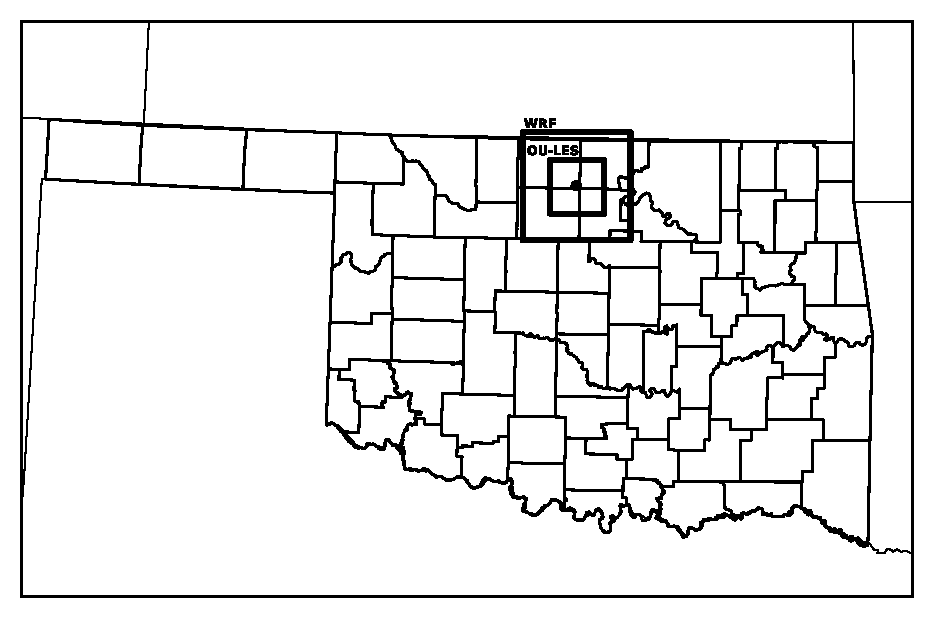
\includegraphics[width=0.9\textwidth]{figures/chapter4/domains}
\end{center}
\caption{WRF model domain with $1$-$\kilo\metre$ grid spacing (outer square) and OU-LES domain (inner square) centered over the LMN site (indicated with a dot).}
\label{figure01}
\end{figure}


Model specifications, setup details, and verification approach are presented in Sections \autoref{ed-41} and \autoref{vt-42}. The investigated CBL cases are described in the subsequent sections, in which model predictions of CBL flow are analyzed in comparison with observational and OU-LES data. Section \autoref{dis-48} contains summary and conclusions.

\section{Experimental Design}
\label{ed-41}

\subsection{University of Oklahoma Large Eddy Simulations}
\label{les-411}

Large eddy simulations were conducted in a numerical domain with size $51.1 \times 51.1 \times 4$ $\kilo\metre^3$ centered over the Lamont site, with horizontal spacing $\Delta x = \Delta y = 100$ $\metre$ and vertical spacing $\Delta z = 50$ $\metre$. The first model level was located at $25\, \metre$ above ground level (AGL). Surface fluxes in the simulations were prescribed from the eddy correlation flux measurement system (ECOR; \citealt{armECOR}) at the Lamont site, with flux values available in 30-minute intervals. To account for the larger-scale (as compared to the size of the LES domain) atmospheric variability, a force-restore nudging procedure was implemented in the OU-LES. The solutions for horizontal velocity components, virtual potential temperature, and water vapor mixing ratio at each time step were nudged with temporally interpolated profiles (soundings) from the Rapid Update Cycle (RUC; \citealt{RUC}) model. The following force-restore (f-r) term was incorporated in the filtered LES equations:


\be
\left(\pd{\tilde{\phi}}{t}\right)_{\textrm{f-r}} = - \frac{\overline{\tilde{\phi}}(z)_{\textrm{LES}} - \phi(z)_{\textrm{RUC}}}{t_{\textrm{r}}} \mbox{ ,}
\ee
\noindent
where $\tilde{\phi}$ is the considered resolved (i.e.\ filtered in the LES sense) flow variable, $\left(\partial \tilde{\phi} / \partial t\right)_{\textrm{f-r}}$ is its tendency due to the nudging (force-restore mechanism), $\overline{\tilde{\phi}}(z)_{\textrm{LES}}$ is the mean (obtained by averaging over horizontal planes) profile of $\tilde{\phi}$ from the preceding time step, $\phi(z)_{\textrm{RUC}}$ is the RUC profile of the flow variable at that time step, and $t_{\textrm{r}}$ is the nudging time constant, which was set equal to $3600$ seconds. Hence, the tendencies of the above specified physical variables are adjusted across the entire domain every time step by subtracting the time-scaled difference between the domain-averaged profiles from OU-LES and the local profile from RUC at the previous time step. The time constant regulates the rate of adjustment of the spatially averaged LES fields to the RUC profiles that represent the larger-scale atmospheric fields.

\subsection{The Weather Research and Forecasting Model}
\label{wrf-412}

The WRF model was employed in two domains (all being centered at the Lamont site), with horizontal grid spacing of $1$ and $4$ $\kilo\metre$. Both domains used the same $101\times101$ horizontal grid with $41$ vertical levels. The first model level was located at 8 $\metre$ above ground level (AGL). All initial and lateral boundary conditions were provided from North American Regional Reanalysis (NARR; \citealt{NARR}) data. A 12-hour warm start was used to allow for model spin-up. The WRF model settings for microphysics, longwave radiation, shortwave radiation, land-surface model, and horizontal diffusion closure were held the same for all model runs. The surface layer (SL) and PBL schemes of the WRF model were varied in conjunction with horizontal grid spacing. For further details on the respective physics packages, refer to Chapter \autoref{wrf-3}.

The physical schemes that are held the constant in the experiments with different SL\slash PBL parameterizations represent a sensible set of physical scheme options in the WRF model. In combination, these schemes serve as a baseline environment to test sensitivity of turbulent flow predictions by the WRF model to SL\slash PBL schemes in conjunction with varying horizontal grid spacing. While one might claim that certain baseline schemes work better than others, it is beyond the purview of this study to evaluate these secondary schemes. It is more important to hold them unchanged so that the WRF model sensitivity to the choice of a SL\slash PBL scheme combination may be more easily discerned.

\section{Verification Techniques}
\label{vt-42}

In modeling studies, the matter of validating model results with data that represent the actual atmospheric state is a recurrent issue. One inherent problem of such a comparison is that model data for one grid cell represent the local atmospheric state as a statistical mean over the cell while observational data are usually collected at a single location arbitrarily positioned with respect to the model grid. In this sense, to compare single-point observations with model results is rather problematic. However, as is the case in this study, if the geographic area over which the comparison is undertaken is (or may be considered) homogeneous in a statistical sense, then the comparison of atmospheric boundary layer flow statistics obtained with different schemes and with different grid spacing appears to be sensible.

In order to facilitate the outlined comparison, the WRF model data were extracted for the subset of cells that coincided with the OU-LES domain. Within this comparison domain, horizontal averages were taken of both WRF model and OU-LES data for each respective output time in order to produce mean vertical profiles over the Lamont site. This proves to be a reasonable approach since the land-surface properties in north-central Oklahoma are fairly homogeneous. For potential temperature and water vapor mixing ratio, both the WRF model and OU-LES data were extrapolated following Monin-Obukhov similarity theory (\citealt{MO}; \citealt{Dyer}) to $2  \mbox { }\metre$ AGL. This level coincided with the measurement height of the ARM surface meteorological observation system (SMOS; \citealt{armSMOS}). For wind speed and direction, both WRF model and OU-LES data were similarly extrapolated to the SMOS observation level of $10 \mbox{ }\metre$ AGL. The extrapolated values were subsequently averaged in time to generate hourly means, which allowed for removal of small-scale temporal perturbations and numerical noise. The resultant data were used to compare parameters of the near-surface atmospheric structure over time periods which carried both mesoscale and synoptic-scale signals. For turbulence fields, WRF model and OU-LES data were compared against both ECOR and the ARM carbon dioxide flux measurement system (CO2FLX; \citealt{armCO2FLUX}). While the Lamont site measurements represent single points in space, their inclusion provides a real-world component for model validation. 

\section{Case 1: June 7, 2007}
\label{june7-43}

\subsection{Meteorological Conditions}
\label{mc-431}


\begin{figure}[H]
     \begin{center}
%
        \subfigure[7 June 2007 12 UTC]{%
            \label{figure402a}
            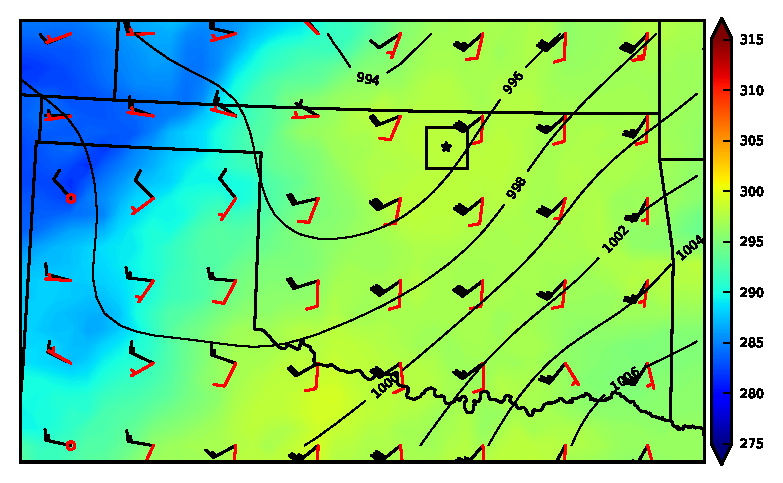
\includegraphics[width=0.5\textwidth]{figures/chapter4/ruc_20070607_12_composite}
        }%
        \subfigure[7 June 2007 16 UTC]{%
           \label{figure402b}
           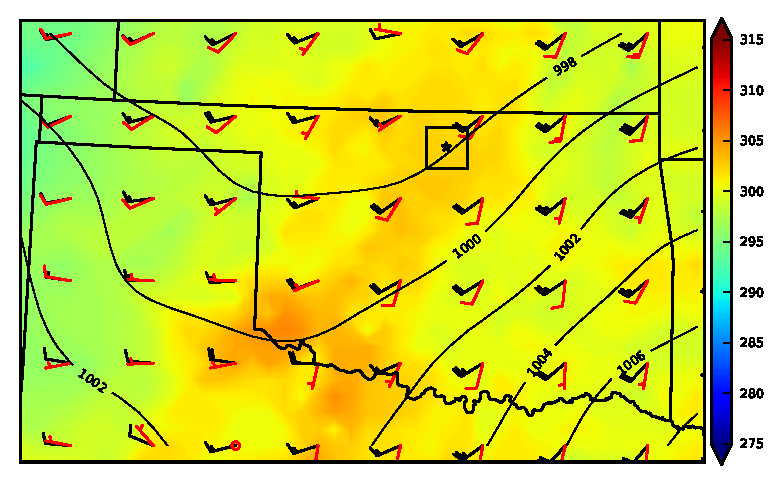
\includegraphics[width=0.5\textwidth]{figures/chapter4/ruc_20070607_16_composite}
        }\\ %  ------- End of the first row ----------------------%
        \subfigure[7 June 2007 20 UTC]{%
            \label{figure402c}
            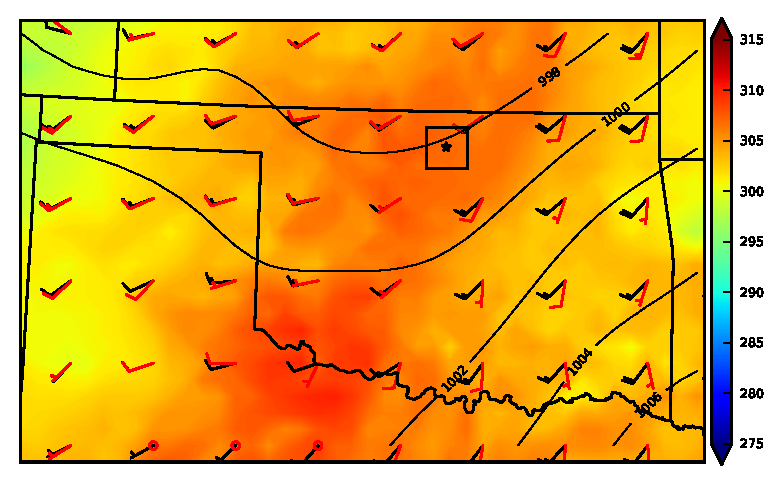
\includegraphics[width=0.5\textwidth]{figures/chapter4/ruc_20070607_20_composite}
        }%
        \subfigure[8 June 2007 00 UTC]{%
            \label{figure402d}
            \includegraphics[width=0.5\textwidth]{figures/chapter4/ruc_20070608_00_composite}
        }%
%
    \end{center}
    \caption{%
        Meteorological conditions taken from RUC analyses for 7 June 2007. Surface pressure ($\hecto\pascal$) is the contoured quantity, surface temperature ($\kelvin$) is the shaded quantity, and surface winds and $850\hecto\pascal$ winds ($\metre\reciprocal\second$) are the red and black wind barbs, respectively. The black square represents the comparison domain, while the black star depicts the location of the Lamont, Oklahoma ARM profiler site.}%
   \label{figure402}
\end{figure}


The first investigated CBL case was simulated from 1300 UTC (0800 local time) 7 June 2007 to 0000 UTC (1900 local time on 7 June) 8 June 2007. This time interval roughly corresponds to the local summer daytime. Few, if any, clouds were present in the CBL over this period of time. The absence of clouds resulted in strong surface heating and was accompanied by moderate to strong winds. As a consequence, a deep sheared CBL developed during the course of the day. These conditions are representative of the CBL type that is known to be confidently reproduced by the OU-LES code. 

Figure~\ref{figure402} illustrates the temporal evolution of meteorological conditions across Oklahoma and the immediately surrounding areas. At the beginning of the simulation period, a surface low-pressure system was situated in South Dakota. A cold front extended from South Dakota southwestward into New Mexico. The cold front intersected Oklahoma in the central portion of the panhandle. A dryline extended from this cold front southward into the central portion of the Texas panhandle. Surface winds across the region were from the south at $10\mbox{ }\metre\reciprocal\second$. Throughout the depth of the boundary layer, winds veered with increasing height as $850\mbox{ }\hecto\pascal$ winds were from the southwest at $30\mbox{ }\metre\reciprocal\second$. Accordingly, there existed pronounced wind shear in the boundary layer. 

As the day progressed, the dryline propagated eastward, allowing for rapid heating of dry air to the west. By 18 UTC, the dryline passed through the comparison domain and skies cleared. Surface winds shifted to southwesterly behind the dryline and weakened. Ahead of the dryline, winds remained southerly at $10\mbox{ }\metre\reciprocal\second$. Winds at $850\mbox{ }\hecto\pascal$ remained southwesterly but reduced in magnitude. Overall, both directional and speed shear within the CBL were greater within the comparison domain ahead of the dryline than behind.

By the end of the simulation period at 00 UTC on June 8, 2008, the dryline remained east of the comparison domain. Surface winds were westerly behind the dryline and southerly preceding the dryline, with speeds remaining between $5$ and $10\mbox{ }\metre\reciprocal\second$. Throughout the depth of the boundary layer, little shear existed behind the dryline while pronounced directional shear was present in front of the dryline and skies remained clear.

Locally speaking, Fig.~\ref{figure403} shows the atmospheric soundings at Lamont for 1200, 1800, and 0000 UTC. Initially in the course of CBL development, a strong southwest low-level jet (LLJ) was present. The potential temperature profile indicated a stably stratified layer near the surface, resulting from the traditional nocturnal inversion. The near-surface humidity was relatively high, while a dryline formed to the west of the Lamont site and began to propagate eastward. By midmorning into early afternoon, the dryline passed through the site, which resulted in the associated decrease in low-level moisture. Within the CBL, wind speed and shear also decreased. This CBL case is particularly interesting because it allows one to evaluate the ability of the WRF model to reproduce a highly temporally heterogeneous environment in which the combined shear and buoyancy forcing drive CBL growth.


\begin{figure}[H]
\begin{center}
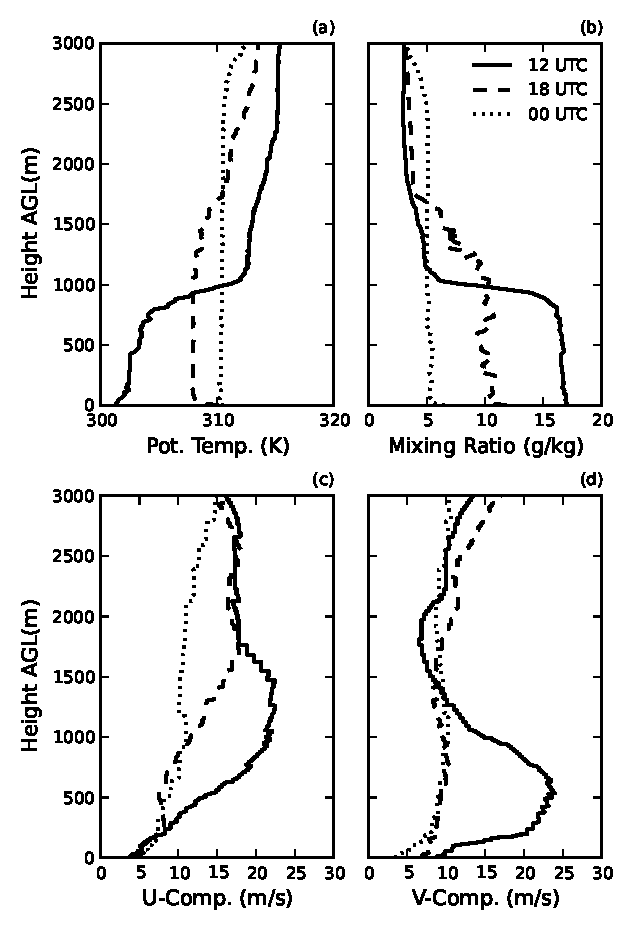
\includegraphics[width=0.5\textwidth]{figures/chapter4/20070607_lmnsounding}
\end{center}
\caption{Atmospheric soundings at the LMN site for 7 June 2007: (a) potential temperature, (b) water vapor mixing ratio, (c) x component of wind, and (d) y component of wind. Solid, dashed, and dotted lines correspond, respectively, to 1200, 1800, and 0000 (following day) UTC.}
\label{figure403}
\end{figure}


\subsection{Results}
\label{res-432}

Figure~\ref{figure404} illustrates the effects of changing grid spacing for potential temperature, water vapor mixing ratio, wind speed, and wind direction. Keeping in mind that WRF model values at 13 UTC represent a $12$-hour forecast due to the warm-start procedure, potential temperature and water vapor mixing ratio values were smaller than observational values for all schemes. As the day progressed, WRF model predictions for potential temperature continued to exhibit smaller values than observations, while predicted water vapor mixing ratio values were too small (large) prior to (following) the dryline passage. For both potential temperature and mixing ratio, the WRF model time evolution matched the physical trend better than did OU-LES, which was unable to reproduce the relatively sharp changes in the meteorological fields associated with dryline motion. This inability of OU-LES to treat boundary layer flows with sharp gradients of meteorological fields along the simulation domain has been marked out in  \citet{Confe2008}. Differences among model outputs with different grid spacing values were rather small for each scheme, with model runs using $4$-$\kilo\metre$ spacing often comparing more favorably with observations for potential temperature. Modeled horizontal wind speed values were systematically underpredicted, for all turbulence scheme and grid spacing combinations. When differences between outputs with disparate grid spacing values were notable, model configurations employing $4$-$\kilo\metre$ spacing reproduced values closer to observations. Wind direction estimates were nearly identical to observations and OU-LES data for all scheme and spacing combinations, with rather inconsequential differences related to grid-spacing variations.


\begin{figure}[ht!]
\begin{center}
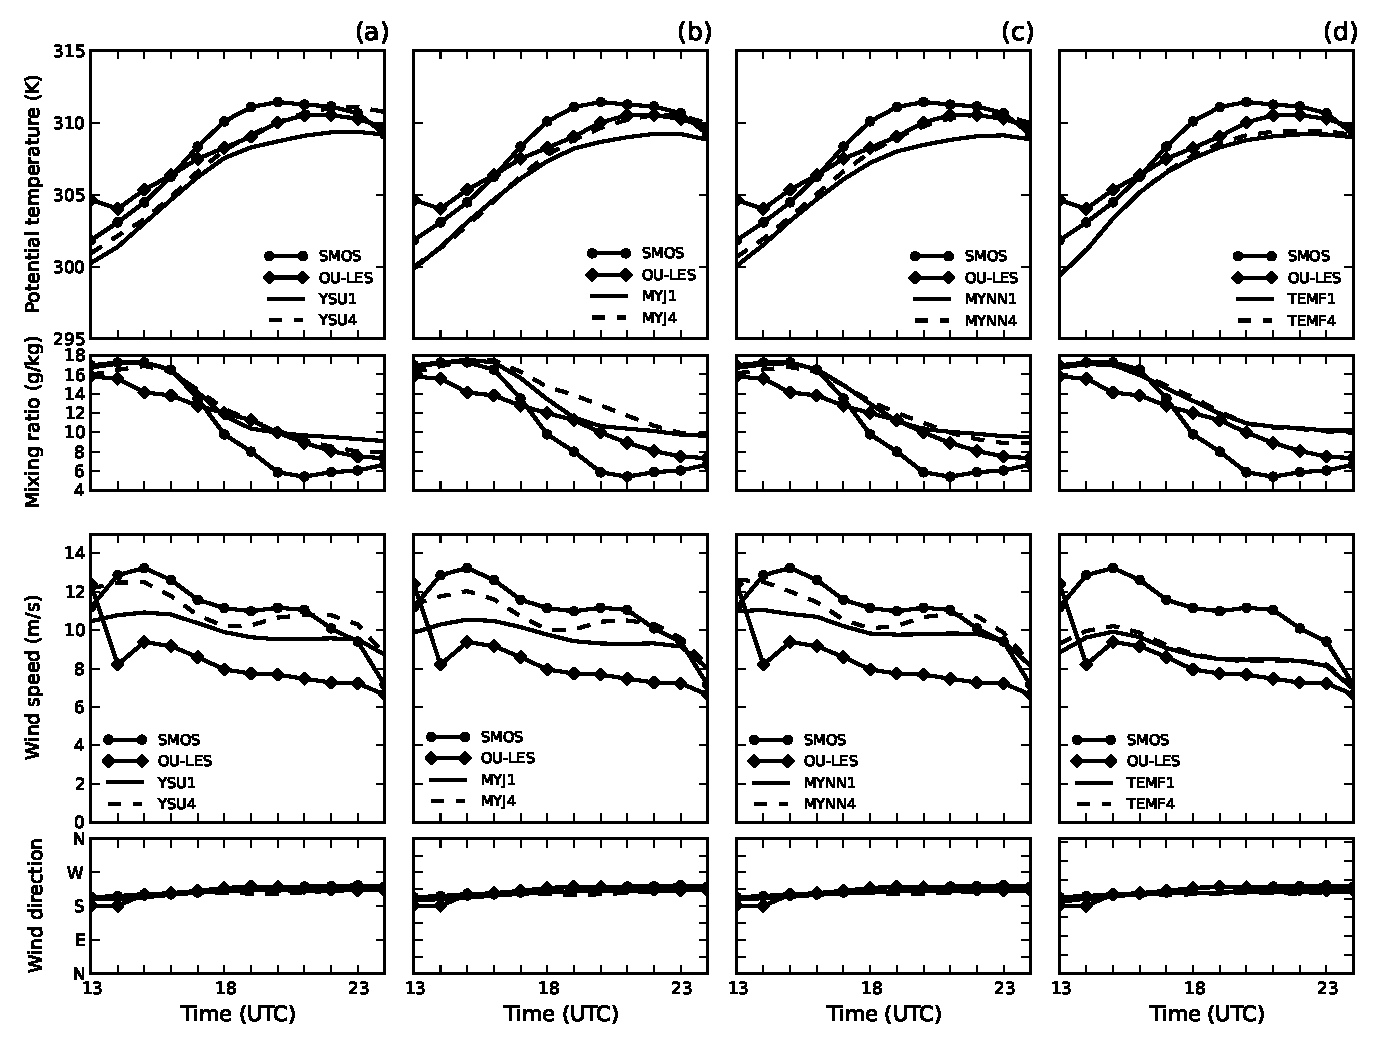
\includegraphics[width=\textwidth]{figures/chapter4/meteogram_grid_20070607}
\end{center}
\caption{Evolution of potential temperature (top row), water vapor mixing ratio (second row), wind speed (third row), and wind direction(bottom row) predicted by the WRF model with (left to right) different parameterization schemes and different grid spacings (denoted by the number after the scheme label in the keys) for 7 June 2007. Observational (SMOS) and OU-LES data are also shown for comparison.}
\label{figure404}
\end{figure}


Comparison of model flux predictions with Lamont observations yielded somewhat striking discrepancies. Because the OU-LES was driven with surface fluxes observed at the Lamont site, it would be redundant to include here for comparison surface flux values from the corresponding simulations. Surface sensible heat flux values predicted by the WRF model were systematically and significantly lower as compared with the observed values, while surface latent heat flux values were grossly overestimated. However, discrepancies between model predictions with different grid spacings were rather small and inconsequential (hence, the corresponding data are not shown). The noted large discrepancies in sensible and latent flux values are discussed below. 

The WRF model predictions for turbulence velocity scale and turbulence temperature scale are of importance for many practical applications that employ near-surface turbulence parameters. One such example is evaluating the properties of electromagnetic and sound wave propagation in the atmospheric surface layer. Figure~\ref{figure405} illustrates the effects of changing grid spacing on turbulence parameters among the four investigated WRF model PBL schemes. Time evolution of $u_*$ predictions from all WRF model configurations closely match phase with observations and are closer to observed values than OU-LES. Each configuration produces a systematic overprediction when compared with observed values, except for the TEMF scheme which yields significantly lower values. The behavior of $\theta_*$ predictions match the phase of the observational time trace. All employed combinations of SL\slash PBL schemes and grid spacings systematically underpredict $\theta_*$ as compared with both OU-LES and Lamont data, while differences among schemes are consistently small. In general, refined grid spacing in this particular case led to slightly more realistic model predictions of both $u_*$ and $\theta_*$. 


\begin{figure}[ht!]
\begin{center}
\includegraphics[width=\textwidth]{figures/chapter4/ust_tst_grid_20070607}
\end{center}
\caption{Evolution of (top) friction velocity $u_*$ and (bottom) temperature scale $\theta_*$ predicted by the WRF model with (left to right) different parameterization schemes and different grid spacings (denoted by the number after the scheme label in the keys) for 7 June 2007. Observational (ECOR and CO2FLX) and OU-LES data are also shown for comparison.}
\label{figure405}
\end{figure}


Values for CBL depth estimates were smaller for all WRF model configurations early in the simulation window as compared with both OU-LES and observational data. As the day progressed, the PBL depth estimates from the WRF model became more consistent with observational data. In all cases, reducing the grid spacing led to more realistic depth estimates. Except for the beginning and ending periods of the simulation window, all WRF model predictions of the stability parameter matched rather closely with both OU-LES and observational data. Given the previously discussed behavior of $u_*$, such discrepancies should be expected. Differences between WRF model predictions with different grid spacing were inconsequential during portions of the day with peak convective activity (the corresponding data are not shown). 

Figure~\ref{figure406} illustrates a meteogram (timeline trace) of basic meteorological variables derived from WRF model output, OU-LES data, and measurements at the Lamont site. Remembering that the 13 UTC values from WRF model represent conditions achieved after 12-hour spin-up, while OU-LES is initialized with local 13 UTC profiles retrieved from the RUC data, one immediately notes a common problem for employed SL\slash PBL schemes in the WRF model at the beginning of the day: they all predict cooler and slightly drier atmospheric conditions as compared with the observed values for temperature and water vapor mixing ratio. The WRF model more confidently reproduces the sharp decrease in moisture associated with the dryline passage with the YSU scheme, while remaining schemes fail to capture the evolution pattern. The OU-LES code predicts much more gradual changes in the mixing ratio than the observations show. In both cases, however, the magnitude of the moisture drop is not well reproduced. Wind speed and direction predictions with different schemes are rather close to each other, with MYNN and YSU schemes producing results slightly closer to observations than the MYJ and TEMF scheme. Wind speeds from the WRF model are closer to observational data than OU-LES. Although the speed values are underpredicted, they closely match the semidiurnal pattern of the wind. 


\begin{figure}[ht!]
\begin{center}
\includegraphics[width=\textwidth]{figures/chapter4/meteogram_phys_20070607}
\end{center}
\caption{Evolution of (a) potential temperature (upper panel) and water vapor mixing ratio (lower panel) and (b) wind speed (upper panel) and wind direction (lower panel) predicted by the WRF model with different parameterization schemes for 7 June 2007. Observational (SMOS) and OU-LES data are also shown for comparison.}
\label{figure406}
\end{figure}


Drastic differences between WRF model predictions and observational heat-flux data are evident in Fig.~\ref{figure407}. The surface sensible heat flux is hugely underpredicted, while the surface latent heat flux is grossly overpredicted. However, one can examine total heat flux (sensible flux added to latent flux), for which data are consistent with each other and with anticipated variations of the surface buoyancy flux in the clear CBL at the Lamont site. This points to an apparent heat flux partition problem in the modeled CBL. The exact cause of this problem is not clear, but it is possibly a culprit of the LSM employed in the WRF model. For sensible heat flux the TEMF scheme is furthest from observations than the other three schemes. For latent heat flux, the YSU scheme matches most closely with observed values, while the TEMF scheme differs the most.


\begin{figure}[ht!]
\begin{center}
\includegraphics[width=\textwidth]{figures/chapter4/shf_lhf_phys_20070607}
\end{center}
\caption{Evolution of the near-surface (a) sensible, (b) latent, and (c) total heat fluxes predicted by the WRF model with different parameterization schemes for 7 June 2007. Observational data (ECOR and CO2FLX) are also shown for comparison.}
\label{figure407}
\end{figure}


The noted discrepancies in flux partitioning are disconcerting. Among the physics schemes that are held constant in the WRF model runs, one can easily argue that the LSM is most closely tied to the SL\slash PBL schemes. Accordingly, all studied cases were rerun using the Pleim-Xiu (PX) LSM ~\citep{PleimXiu95, XiuPleim01} in place of the Noah LSM with the hope of resolving the partitioning issue. Results from these simulations are not shown here for sake of brevity. The PX LSM produces a smaller latent heat flux that is closer to the observational data from the LMN site. The corresponding values of the sensible heat flux are slightly larger and closer to observations than values obtained with the Noah LSM, although the change is somewhat modest. This seems to be a desirable tendency. However, closer inspection of produced soil moisture values temper this finding. The Noah LSM appears to better reproduce soil moisture than does the PX LSM. This means that departing farther from observations, soil moisture produced with the PX scheme artificially improves the latent flux values with the flux-partitioning error still in place. These findings present an example of what a typical user may encounter while modeling meteorological conditions considered in this case. In an applied framework, the unnatural correction of the model to account for this error is simply not practical or physically coherent.

Turbulence scales for velocity and temperature are shown in Fig.~\ref{figure408}. Both OU-LES and the WRF model produce $u_*$ values generally consistent with observational data. When differences do exist, the WRF model values are larger, thus overpredicting the mechanical turbulence generation. The YSU, MYJ, and MYNN schemes predict values closer to observations than the TEMF scheme, although results with all four schemes follow the same evolution pattern. The magnitude of the turbulence temperature scale is underestimated by all four SL\slash PBL schemes in the WRF model, as compared with OU-LES values that agree with Lamont observational data rather decently. Such behavior of the modeled $\theta_*$ is quite expectable given the modest WRF-model overprediction of friction velocity and the underprediction of surface sensible heat fluxes. Differences among predictions with distinct SL\slash PBL schemes are rather minor, with the TEMF scheme predicting values closest to observations.


\begin{figure}[ht!]
\begin{center}
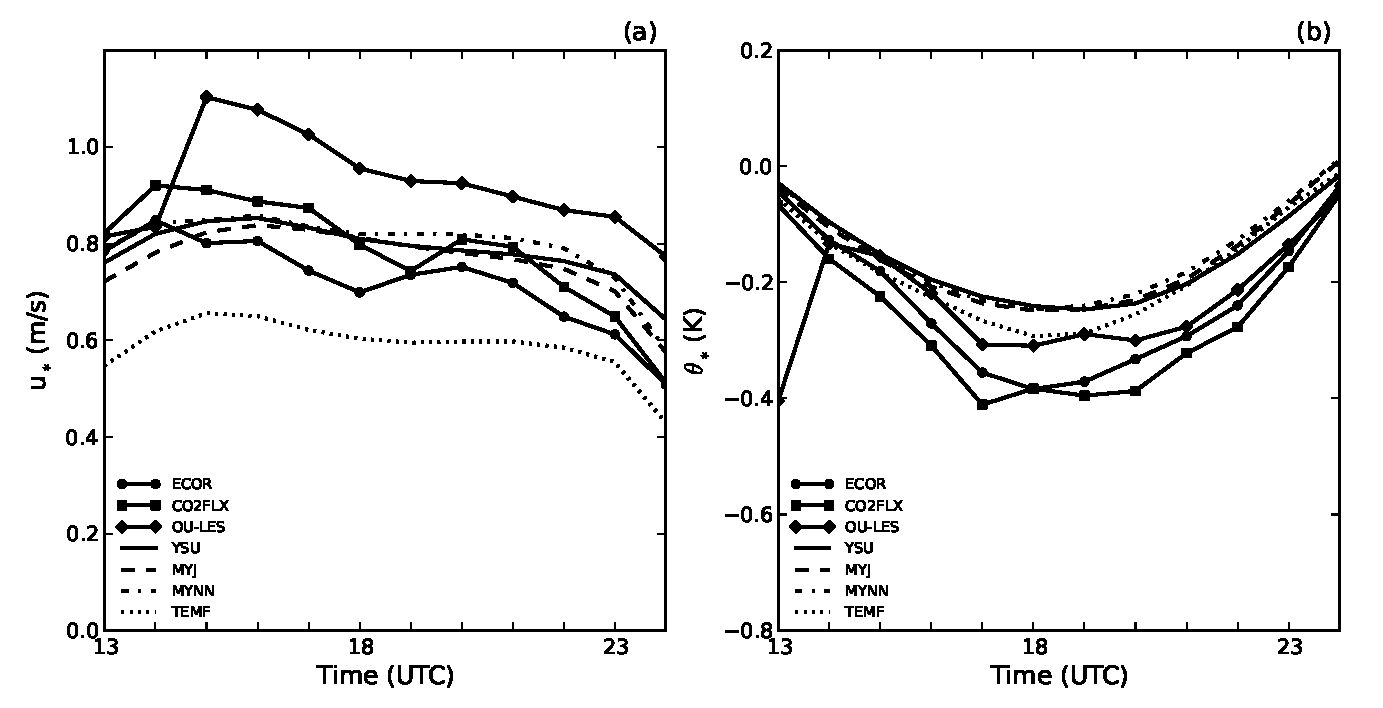
\includegraphics[width=\textwidth]{figures/chapter4/ust_tst_phys_20070607}
\end{center}
\caption{Evolution of the (a) friction velocity $u_*$ and (b) temperature scale $\theta_*$ predicted by the WRF model with different parameterization schemes for 7 June 2007. Observational data (ECOR and CO2FLX) and OU-LES data are also shown for comparison.}
\label{figure408}
\end{figure}


When inspecting Fig.~\ref{figure409}, it may appear at first glance that the SL\slash PBL schemes in the WRF model produce too sharp an increase of the CBL depth. However, given that there are only two available data points from the Lamont site that provide estimates of the CBL depth, and taking into account the previously noted OU-LES failure to capture sharp changes in meteorological fields associated with the dryline passage, it is entirely possible that the WRF model more accurately represents the CBL depth evolution than OU-LES does. Differences among predictions are rather small, while the TEMF scheme produces the shallowest CBL early into the day and the YSU scheme predicts the deepest CBL during peak growth. In terms of the stability parameter, $\zeta = -z_i / L$, the YSU, MYJ, and MYNN schemes produce values close to the OU-LES results for times of peak convective activity, and predict weaker buoyancy contribution to the CBL turbulence regime than the observations indicate. Oppositely, the TEMF values are significantly larger, undoubtedly a result of significant underprediction of the shear contribution. 


\begin{figure}[ht!]
\begin{center}
\includegraphics[width=\textwidth]{figures/chapter4/pblh_phi_phys_20070607}
\end{center}
\caption{Evolution of (a) $z_i$ and (b) stability parameter $-\frac{z_i}{L}$ predicted by the WRF model with different parameterization schemes for 7 June 2007. Observational (LMN, ECOR, and CO2FLX) and OU-LES data are also shown (for unstable conditions only).}
\label{figure409}
\end{figure}


\section{Case 2: September 27, 2008}
\label{sept27-44}

\subsection{Synoptic Conditions}
\label{mc-441}


\begin{figure}[H]
     \begin{center}
%
        \subfigure[27 September 2008 12 UTC]{%
            \label{figure403a}
            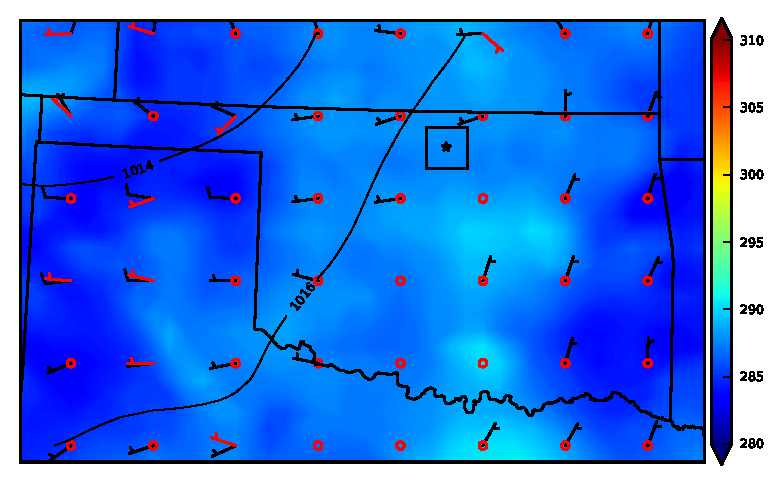
\includegraphics[width=0.5\textwidth]{figures/chapter4/ruc_20080927_12_composite}
        }%
        \subfigure[27 September 2008 16 UTC]{%
           \label{figure403b}
           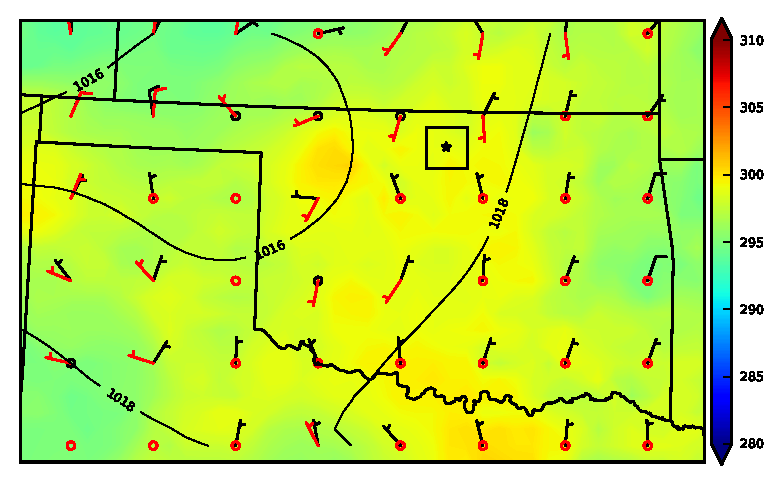
\includegraphics[width=0.5\textwidth]{figures/chapter4/ruc_20080927_16_composite}
        }\\ %  ------- End of the first row ----------------------%
        \subfigure[27 September 2008 20 UTC]{%
            \label{figure403c}
            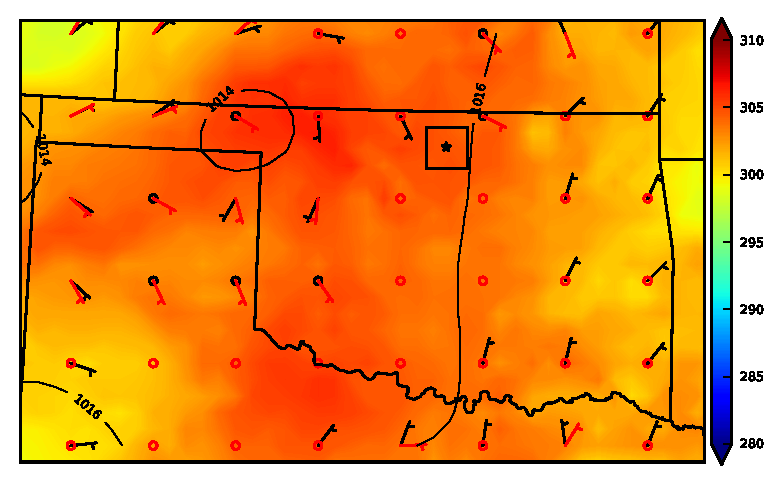
\includegraphics[width=0.5\textwidth]{figures/chapter4/ruc_20080927_20_composite}
        }%
        \subfigure[28 September 2008 00 UTC]{%
            \label{figure403d}
            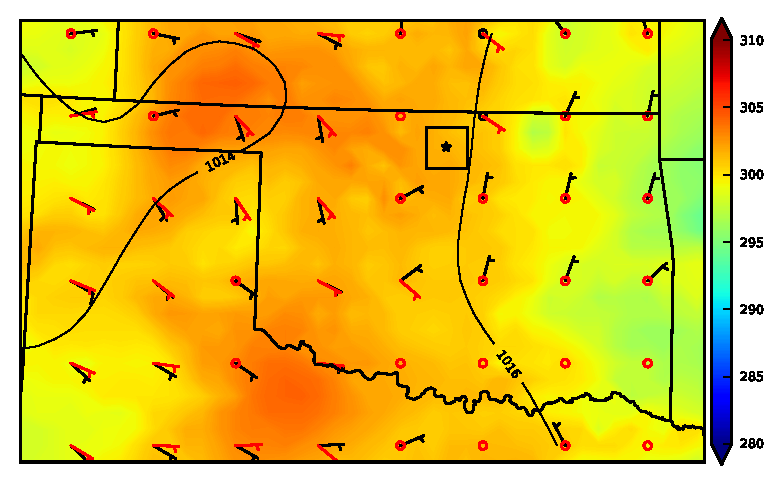
\includegraphics[width=0.5\textwidth]{figures/chapter4/ruc_20080928_00_composite}
        }%
%
    \end{center}
    \caption{%
        Meteorological conditions taken from RUC analyses for 27 September 2008. Surface pressure ($\hecto\pascal$) is the contoured quantity, surface temperature ($\kelvin$) is the shaded quantity, and surface winds and $850\hecto\pascal$ winds ($\metre\reciprocal\second$) are the red and black wind barbs, respectively. The black square represents the comparison domain, while the black star depicts the location of the Lamont, Oklahoma ARM profiler site.}%
   \label{figure410}
\end{figure}


The second investigated CBL case was simulated from 1400 UTC (0900 local time) 27 September 2008 to 2300 UTC (1800 local time) 27 September 2008. Over this period of time, the CBL was primarily free of clouds. The absence of clouds allowed relatively strong surface heating. Unlike the first studied CBL case, this particular CBL contained relatively weak winds. Consequently, a deep, well-mixed CBL developed during the course of the day, mostly driven by buoyancy forcing. Any shear present in this case was largely directional in nature. These conditions are, again, representative of the CBL type that is known to be confidently reproduced by the OU-LES code. 

The temporal evolution of meteorological conditions across the Oklahoma geographical region is depicted in Fig.~\ref{figure410}. At the beginning of the simulation period, a weak cold front was present to the north of Oklahoma. Surface winds were weak and variable, and did not appreciably vary throughout the depth of the CBL in terms of direction and speed. At $850\mbox{ }\hecto\pascal$, winds were generally from the west at a speed of $5\mbox{ }\metre\reciprocal\second$. 

Further into the day, a cold front propagated into the Oklahoma panhandle. Surface winds remained variable to $5\mbox{ }\metre\reciprocal\second$ from the southwest, while winds at $850\mbox{ }\hecto\pascal$ were variable to $5\mbox{ }\metre\reciprocal\second$ from the north-northeast, thus indicating some unorganized directional shear throughout the CBL. Any shear associated with speed was largely absent. Accordingly, heating in the lowest layers of the CBL was supported. Meanwhile, a high-pressure system strengthened to the west and began movement toward the central plains.

By the end of the simulation period at 2300 UTC on September 27, 2008, the previously observed weak surface boundary in the Oklahoma panhandle transitioned into a stationary front. The high-pressure system to the west of the domain continued its movement eastward into the central plains. Winds remained light and variable throughout the boundary layer, with a slight shift to the south-southeast. Again, shear effects on boundary layer development were tempered. Surface heating slowed and temperatures slightly cooled. Other bulk meteorological fields remained noticeably steady.

Figure~\ref{figure411} shows atmospheric soundings for Lamont at 1200, 1800, and 0000 UTC. Initially, the nocturnal inversion remained in place, marked by a stable-stratified region near the surface. Low-level moisture was modest and slightly increased with height. Winds were fairly weak and from the southwest. With the low-pressure system to the north of Oklahoma stalling, the wind field remained largely unchanged. Surface heating persisted and turbulent transport by buoyancy forces dominated the CBL growth. Through time, winds weakened, temperatures remained steady, and the air became subtly drier as a well-mixed boundary layer developed, though with a more modest depth than the first investigated case. This CBL provides an interesting case to investigate because unlike the CBL present on June 7, 2007, it examines the WRF model's ability to reproduce a relatively stationary system in which buoyancy forcing is the primary driving mechanism for boundary layer growth.


\begin{figure}[H]
\begin{center}
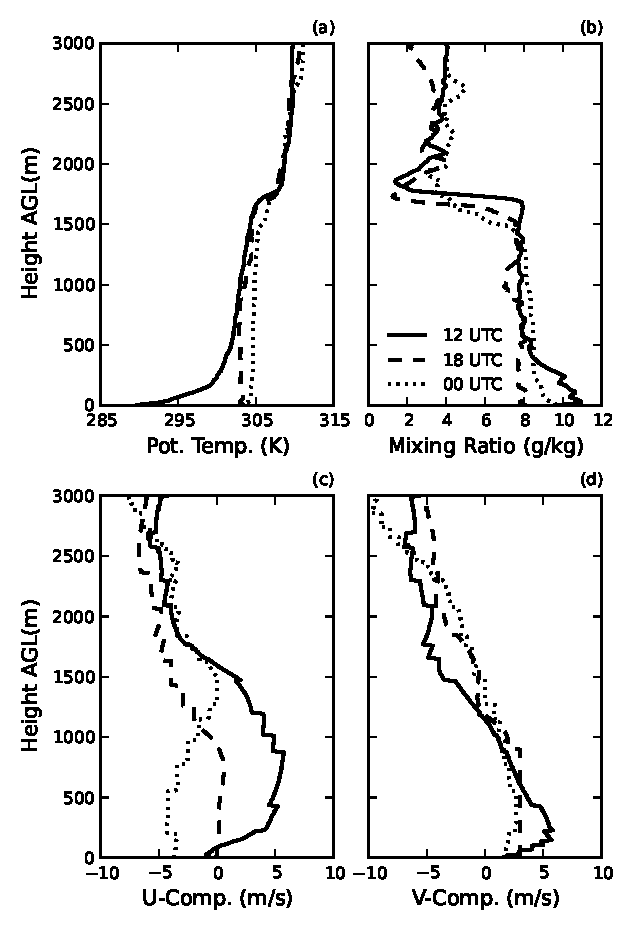
\includegraphics[width=0.5\textwidth]{figures/chapter4/20080927_lmnsounding}
\end{center}
\caption{Atmospheric soundings at the LMN site for 27 September 2008: (a) potential temperature, (b) water vapor mixing ratio, (c) x component of wind, and (d) y component of wind. Solid, dashed, and dotted lines correspond, respectively, to 1200, 1800, and 0000 (following day) UTC.}
\label{figure411}
\end{figure}


\subsection{Results}
\label{res-442}

Figure~\ref{figure412} illustrates the effects of changing grid spacing for potential temperature, water vapor mixing ratio, wind speed, and wind direction. Potential temperature and moisture values were initially lower than observational and OU-LES data, similar to findings in the first considered CBL case. This may point to a tendency within the WRF model to systematically predict temperatures that are too low during overnight hours (e.g.\ stable conditions). For all schemes, the WRF model predicted values for potential temperature were lower than observational and OU-LES data, although the shape of the time evolution matched rather closely. It should be noted that the TEMF scheme used in conjunction with $4$-$\kilo\metre$ grid spacing produced potential temperature values much closer to observations than any other WRF model configuration. For both the potential temperature and mixing ratio, OU-LES time evolution matched the physical trend better than did the WRF model. Differences among model outputs with varying grid spacing values were more appreciable than in the June 7, 2007 case. Model runs using $4$-$\kilo\metre$ spacing compared more favorably with observations for potential temperature and water vapor mixing ratio than did those using $1$-$\kilo\metre$ spacing. Modeled horizontal wind speed values were systematically underpredicted for all turbulence scheme and grid spacing combinations. When differences between outputs with disparate grid spacing values were notable, model configurations employing $4$-$\kilo\metre$ spacing more often reproduced values closer to observations. Wind direction estimates were generally consistent with observations for both OU-LES predictions and all scheme\slash spacing combinations employed in the WRF model. Given that winds were generally weak, any differences may illustrate a scenario in which local conditions at the observing site were different than the mean value across the model grid cell. Variations in grid spacing resulted in rather inconsequential improvements.


\begin{figure}[ht!]
\begin{center}
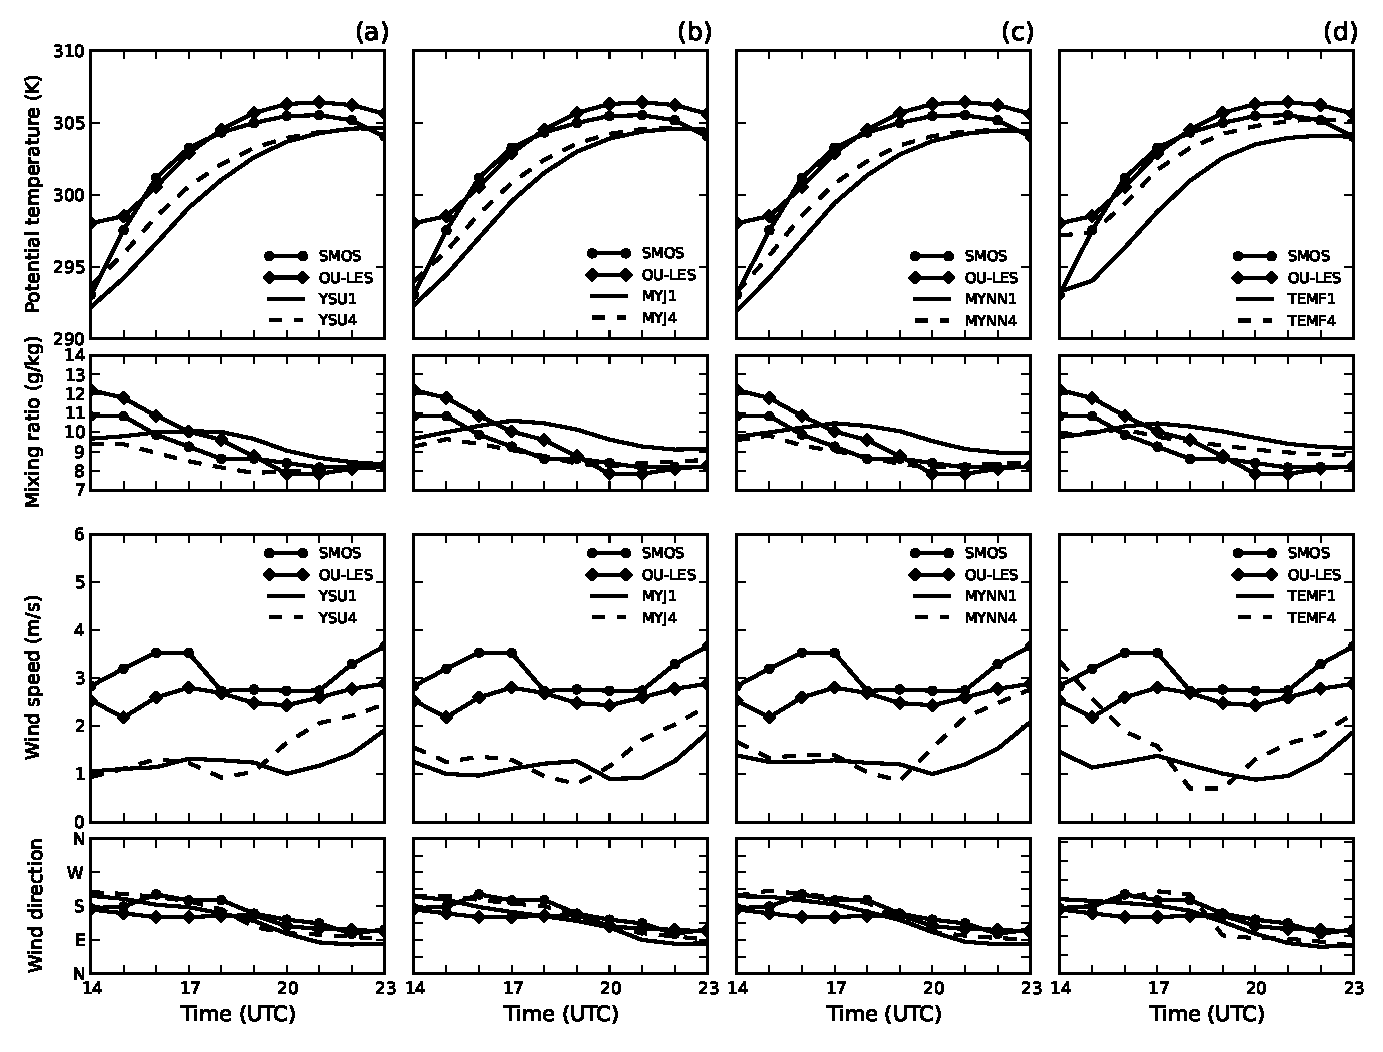
\includegraphics[width=\textwidth]{figures/chapter4/meteogram_grid_20080927}
\end{center}
\caption{Evolution of potential temperature (top row), water vapor mixing ratio (second row), wind speed (third row), and wind direction(bottom row) predicted by the WRF model with (left to right) different parameterization schemes and different grid spacings (denoted by the number after the scheme label in the keys) for 27 September 2008. Observational (SMOS) and OU-LES data are also shown for comparison.}
\label{figure412}
\end{figure}


Comparison of model flux predictions with Lamont observations again yielded somewhat striking discrepancies. Surface sensible heat flux values predicted by the WRF model were systematically lower as compared with the observed values, although differences were generally less pronounced than in the first studied case. Surface latent heat flux values were grossly overestimated. Total flux demonstrated that WRF model predictions were generally consistent with observations. Differences between model predictions with varying grid spacing were rather small and inconsequential (hence, the corresponding data are not shown). The modest discrepancies in sensible heat flux and large differences in latent flux values are discussed below. 

Figure~\ref{figure413} illustrates the effects of changing grid spacing on turbulence parameters among the four investigated WRF model PBL schemes. Time evolution of $u_*$ predictions from all WRF model configurations closely match phase with observations and are generally further from observed values than OU-LES data. Each configuration underpredicts values for friction velocity, with those from the TEMF scheme significantly lower than observational data. The temporal evolution of $\theta_*$ predictions matches the phase of the observational time trace. Every scheme matches closely with observed data and OU-LES predictions, with the lone exception of the TEMF scheme, which grossly overpredicts the magnitude of $\theta_*$. In general, refined grid spacing in this particular case led to inconsequential improvements for model predictions of both $u_*$ and $\theta_*$. 


\begin{figure}[ht!]
\begin{center}
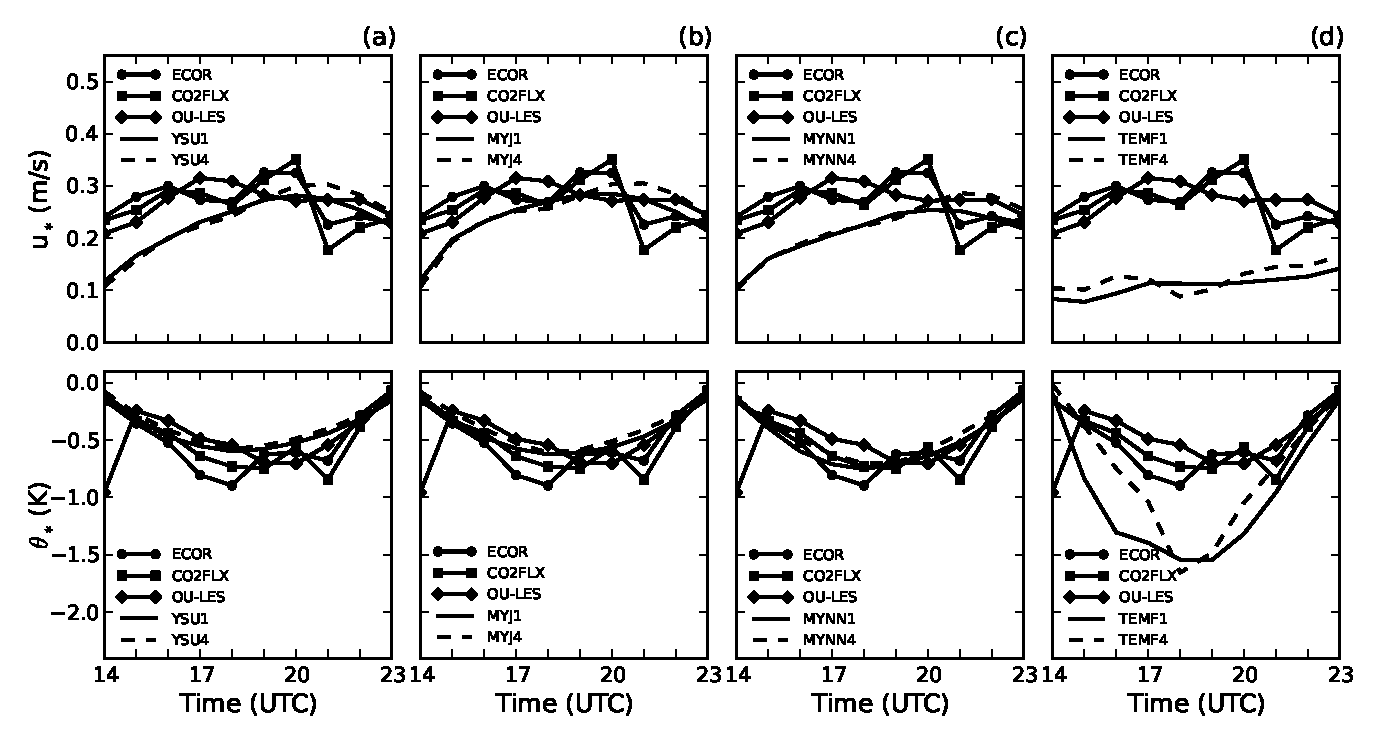
\includegraphics[width=\textwidth]{figures/chapter4/ust_tst_grid_20080927}
\end{center}
\caption{Evolution of (top) friction velocity $u_*$ and (bottom) temperature scale $\theta_*$ predicted by the WRF model with (left to right) different parameterization schemes and different grid spacings (denoted by the number after the scheme label in the keys) for 27 September 2008. Observational (ECOR and CO2FLX) and OU-LES data are also shown for comparison.}
\label{figure413}
\end{figure}


Values for PBL depth estimates were smaller early in the simulation period for all WRF model configurations as compared with OU-LES data. As the CBL developed, the depth estimates from the WRF model became slightly underestimated compared with observations, while those from OU-LES increased prematurely in the simulation period. In all cases, reduction of grid spacing led to more realistic depth estimates. With only one observation time available, it is difficult to surmise how well the stability parameter was predicted throughout the entire simulation time window. However, for the one comparison time, all WRF model predictions except the TEMF scheme were generally close to the observational value. Here, the TEMF scheme overestimated the value by a wide margin, which is not surprising given the associated predictions of friction velocity and turbulence temperature scale. Differences between WRF model predictions with varying grid spacing were inconsequential during portions of the day with peak convective activity (the corresponding data are not shown). 

Figure~\ref{figure414} illustrates a meteogram (timeline trace) of basic meteorological variables derived from WRF model output, OU-LES data, and measurements at the Lamont site. Recalling that the 14 UTC values from WRF model represent conditions achieved after 12-hour spin-up, while OU-LES is initialized with local 14 UTC profiles retrieved from the RUC data, one immediately notes a common problem for employed SL\slash PBL schemes in the WRF model at the beginning of the day: they all predict cooler and drier atmospheric conditions as compared with the observed temperature and water vapor mixing ratio. Such characteristics were discovered in the first investigated CBL case. The OU-LES data better match the diurnal trends for these fields. For potential temperature, there is little difference between schemes, while for water vapor the YSU scheme predicts values closest to observational and OU-LES data. Wind speed and direction predictions with different schemes are rather close to one another, with MYNN and YSU schemes producing values slightly closer to observations than the MYJ and TEMF schemes. Wind speeds from OU-LES are closer to observational data than those from the WRF model. Speed values predicted from the WRF model are again lower than observational and OU-LES data. Wind direction estimates were generally consistent with observations for both OU-LES predictions and all scheme\slash spacing combinations in the WRF model. Any differences may simply illustrate local flow effects that OU-LES and WRF model predictions fail to capture across the entirety of a numerical grid cell.


\begin{figure}[ht!]
\begin{center}
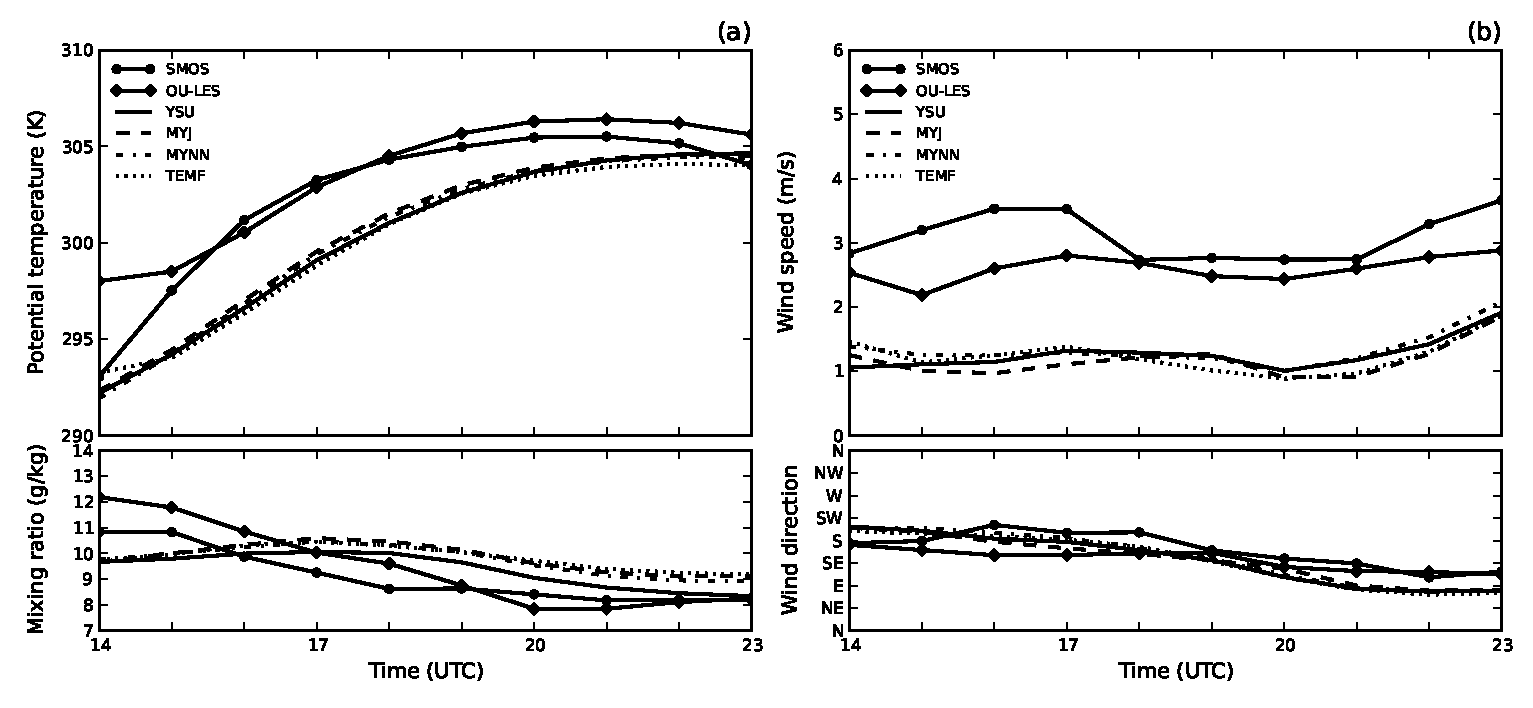
\includegraphics[width=\textwidth]{figures/chapter4/meteogram_phys_20080927}
\end{center}
\caption{Evolution of (a) potential temperature (upper panel) and water vapor mixing ratio (lower panel) and (b) wind speed (upper panel) and wind direction (lower panel) predicted by the WRF model with different parameterization schemes for 27 September 2008. Observational (SMOS) and OU-LES data are also shown for comparison.}
\label{figure414}
\end{figure}


Significant differences between WRF model predictions and observational heat-flux data are evident in Fig.~\ref{figure415}, though such differences are less pronounced than in the June 7, 2007 case. The surface sensible heat flux is underpredicted, while the surface latent heat flux is grossly overpredicted. Examination of the total heat flux shows that several schemes are consistent with observations, with the YSU scheme matching most closely. Such behavior may be indicative of a partitioning problem in the WRF model, an issue with soil moisture representation by the employed LSM, or may simply illustrate local effects that significantly differ from mean behavior within a model grid cell. For sensible heat flux, the YSU scheme is furthest from observations than the other three approaches. For latent heat flux, the YSU scheme is closest to observed values, while the TEMF scheme is the most disparate. 


\begin{figure}[ht!]
\begin{center}
\includegraphics[width=\textwidth]{figures/chapter4/shf_lhf_phys_20080927}
\end{center}
\caption{Evolution of the near-surface (a) sensible, (b) latent, and (c) total heat fluxes predicted by the WRF model with different parameterization schemes for 27 September 2008. Observational data (ECOR and CO2FLX) are also shown for comparison.}
\label{figure415}
\end{figure}


Turbulence scales for velocity and temperature are shown in Fig.~\ref{figure416}. The OU-LES code produces $u_*$ values that are generally consistent with observed values. Oppositely, the WRF model produces values that are too small for all parameterization combinations, thus underpredicting the mechanical turbulence generation. The MYJ and YSU schemes compare most favorably to observations, while the TEMF scheme predicts values that are significantly lower. The magnitude of the turbulence temperature scale is slightly underestimated by the YSU and MYJ schemes, matches closely with the MYNN scheme, and is severely overpredicted by the TEMF scheme. Such behavior of the modeled $\theta_*$ is consistent with each scheme's respective underprediction of friction velocity and surface sensible heat flux.


\begin{figure}[ht!]
\begin{center}
\includegraphics[width=\textwidth]{figures/chapter4/ust_tst_phys_20080927}
\end{center}
\caption{Evolution of the (a) friction velocity $u_*$ and (b) temperature scale $\theta_*$ predicted by the WRF model with different parameterization schemes for 27 September 2008. Observational data (ECOR and CO2FLX) and OU-LES data are also shown for comparison.}
\label{figure416}
\end{figure}


Figure~\ref{figure417} contains one observational value for which to compare against, so any statements regarding accuracy must remain tepid. As the CBL developed, the depth estimates from the WRF model remained slightly lower as compared with observations, while those from OU-LES prematurely increase at a similar rate in the simulation period. Differences among predictions are indistinguishable. In terms of the stability parameter, $\zeta = -z_i / L$, the YSU, MYJ, and MYNN schemes produce values close to the OU-LES results for times of peak convective activity, and predict weaker shear contribution to the CBL turbulence regime than observations indicate. Oppositely, the TEMF values are significantly larger, undoubtedly a result of significant underprediction of shear forcing and overprediction of buoyancy forcing in the CBL development. 


\begin{figure}[ht!]
\begin{center}
\includegraphics[width=\textwidth]{figures/chapter4/pblh_phi_phys_20080927}
\end{center}
\caption{Evolution of (a) $z_i$ and (b) stability parameter $-\frac{z_i}{L}$ predicted by the WRF model with different parameterization schemes for 27 September 2008. Observational (LMN, ECOR, and CO2FLX) and OU-LES data are also shown (for unstable conditions only).}
\label{figure417}
\end{figure}


\section{Case 3: October 26, 2008}
\label{oct26-45}

\subsection{Meteorological Conditions}
\label{mc-451}


\begin{figure}[H]
     \begin{center}
%
        \subfigure[26 October 2008 12 UTC]{%
            \label{figure405a}
            \includegraphics[width=0.5\textwidth]{figures/chapter4/ruc_20081026_12_composite}
        }%
        \subfigure[26 October 2008 16 UTC]{%
           \label{figure405b}
           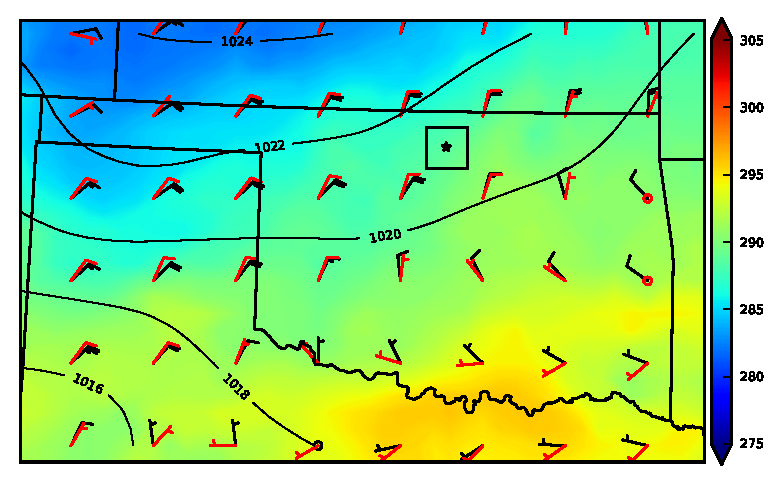
\includegraphics[width=0.5\textwidth]{figures/chapter4/ruc_20081026_16_composite}
        }\\ %  ------- End of the first row ----------------------%
        \subfigure[26 October 2008 20 UTC]{%
            \label{figure405c}
            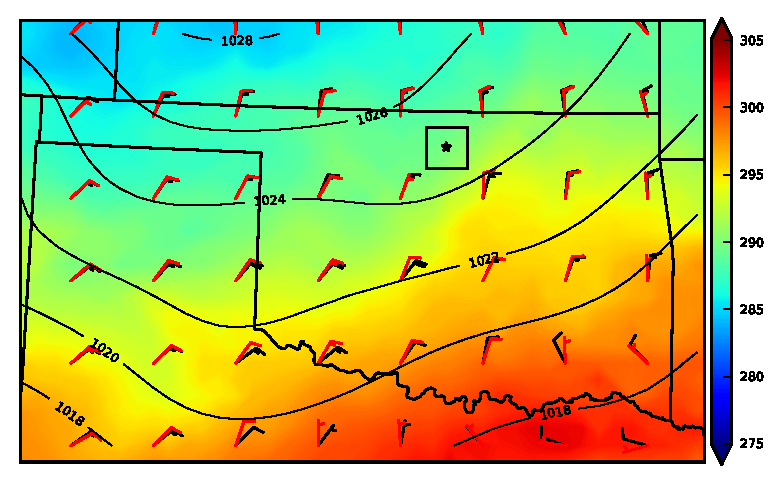
\includegraphics[width=0.5\textwidth]{figures/chapter4/ruc_20081026_20_composite}
        }%
        \subfigure[27 October 2008 00 UTC]{%
            \label{figure405d}
            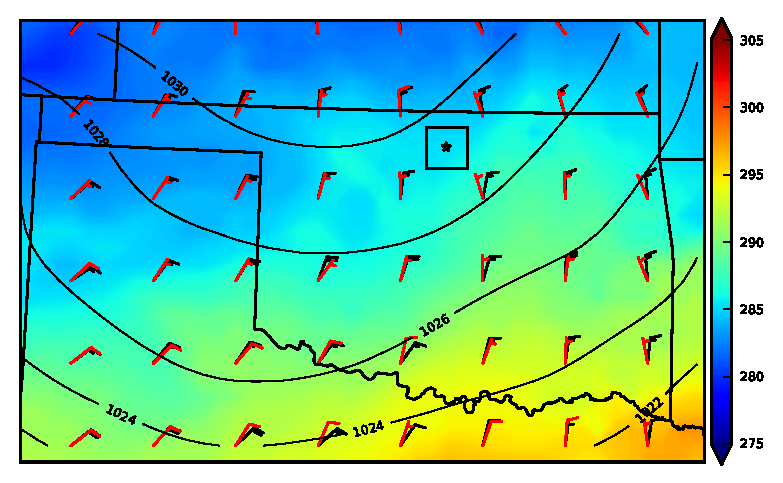
\includegraphics[width=0.5\textwidth]{figures/chapter4/ruc_20081027_00_composite}
        }%
%
    \end{center}
    \caption{%
        Meteorological conditions taken from RUC analyses for 26 October 2008. Surface pressure ($\hecto\pascal$) is the contoured quantity, surface temperature ($\kelvin$) is the shaded quantity, and surface winds and $850\hecto\pascal$ winds ($\metre\reciprocal\second$) are the red and black wind barbs, respectively. The black square represents the comparison domain, while the black star depicts the location of the Lamont, Oklahoma ARM profiler site.}%
   \label{figure418}
\end{figure}


The third investigated CBL case was simulated from 1400 UTC (0900 local time) 26 October 2008 to 2200 UTC (1700 local time) 26 October 2008. Again, these represent times with positive surface heat flux. Like previously investigated cases, this CBL was marked by minimal, if any, cloud cover. Observed during this case were strong shifts in wind throughout the day, with modest speed shear present throughout the CBL. A deep mixed layer developed by the end of the simulation period. Unlike the first two CBL cases, the increasing mean wind acted to limit the organization of such a layer. 

Meteorological conditions present on this particular day are shown in Fig.~\ref{figure418}. At the beginning of the simulation period, a high-pressure system was present in the western United States, while a prominent low-pressure system was centered over the Great Lakes region. Concurrently, a trough extended through central Oklahoma and a cold front spanned Kansas. Surface winds were light and variable, while $850\mbox{ }\hecto\pascal$ winds were from the west at $10\mbox{ }\metre\reciprocal\second$. Accordingly, there existed modest but noticeable speed shear in the boundary layer. 

As the day progressed, the high-pressure system in the west moved southeastward toward Oklahoma. By 16 UTC, the cold front passed through central portions of Oklahoma, bringing associated changes in wind speed and direction. Winds throughout the CBL shifted to the north, with surface values of $10\mbox{ }\metre\reciprocal\second$ and $850\mbox{ }\hecto\pascal$ values of $20\mbox{ }\metre\reciprocal\second$. Overall, directional shear within the CBL was greater ahead of the cold front, while speed shear dominated behind the cold front.

By the end of the simulation period at 2200 UTC on October 26, 2008, the cold front completely progressed through Oklahoma and into Texas. The high-pressure system pushed further into the central plains. The cold front limited surface heating and temperature fields indicated substantial decreases. Winds slightly weakened following the cold frontal passage, with surface values of $5\mbox{ }\metre\reciprocal\second$ and $850\mbox{ }\hecto\pascal$ values of $15\mbox{ }\metre\reciprocal\second$. Once again, directional shear was mostly absent within the CBL, with nearly uniform northerly flow.

Figure~\ref{figure419} shows the local atmospheric soundings at Lamont for 1200, 1800, and 0000 UTC. The initial profile of potential temperature indicated a stably-stratified layer near the surface associated with a nocturnal inversion. Near-surface moisture was much lower than the previously considered CBL cases. Surface winds were light, while mid-level winds were moderate and from the west. By the midmorning, the cold front progressed through the comparison domain. Subsequent profiles of potential temperature and moisture illustrate that warming was mitigated and the atmosphere dried. Additionally, winds depicted a sharp change in speed and direction. Eventually a fairly deep mixed layer formed. However, wind components still exhibited speed shear, which impacted the structure of the well-mixed CBL. This CBL case is interesting because it included a strong wind shift, a frontal passage, and the combined effects of shear and buoyancy forcing to drive CBL growth. 


\begin{figure}[H]
\begin{center}
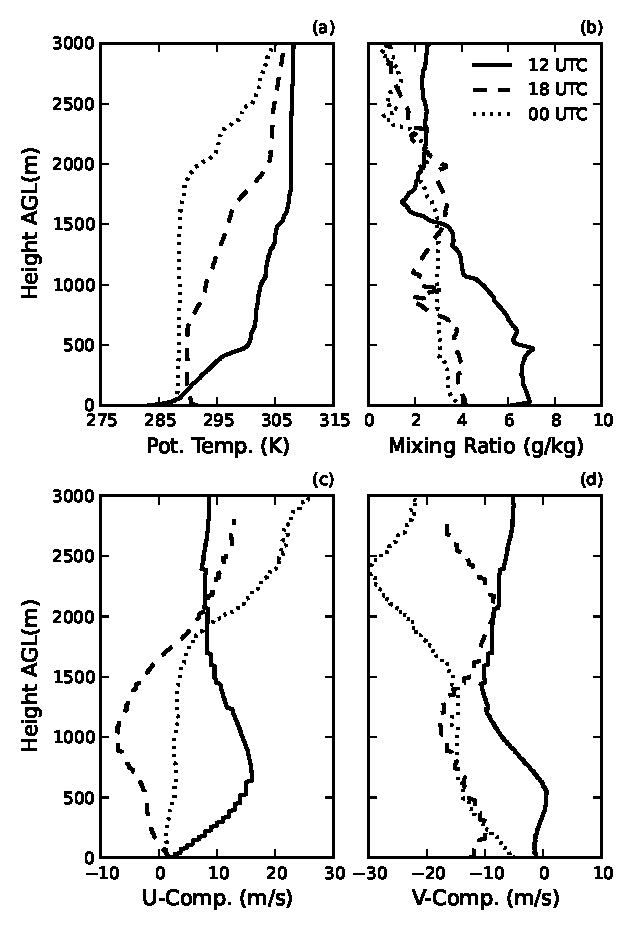
\includegraphics[width=0.5\textwidth]{figures/chapter4/20081026_lmnsounding}
\end{center}
\caption{Atmospheric soundings at the LMN site for 26 October 2008: (a) potential temperature, (b) water vapor mixing ratio, (c) x component of wind, and (d) y component of wind. Solid, dashed, and dotted lines correspond, respectively, to 1200, 1800, and 0000 (following day) UTC.}
\label{figure419}
\end{figure}


\subsection{Results}
\label{res-452}

Figure~\ref{figure420} illustrates the effects of changing grid spacing for potential temperature, water vapor mixing ratio, wind speed, and wind direction. Potential temperature and moisture values were initially lower than observational and OU-LES data, consistent with findings in the previously studied CBL cases. For all schemes, the WRF model predicted values for potential temperature that were lower than observational and OU-LES data for the first half of the simulation period, while the opposite was true for the second half. Meanwhile, the shape of the time evolution matched rather closely. For both the potential temperature and mixing ratio, OU-LES time evolution matched the physical trend slightly better than did the WRF model. Differences among model outputs with varying grid spacing values were small but measurable. Model runs using $4$-$\kilo\metre$ spacing compared more favorably with observations for potential temperature over the first half of the day, while those employing $1$-$\kilo\metre$ spacing fared better for the remainder of the day. For water vapor mixing ratio, those runs using $4$-$\kilo\metre$ spacing compared more favorably with observations for the entirety of the simulation window. Modeled horizontal wind speed values were underpredicted by all turbulence scheme and grid spacing combinations for the first one-third of the day, after which values matched closely with observed data. When differences between outputs with disparate grid spacing values were notable, model configurations employing $4$-$\kilo\metre$ spacing more often reproduced values closer to observations. Wind direction estimates were noticeably different than observations and OU-LES predictions for all scheme\slash spacing combinations in the WRF model over the first one-third of the simulation period. Across the remainder of the day, there was little difference among all predictions of wind direction with observational data. Variations in grid spacing resulted in rather inconsequential improvements.


\begin{figure}[ht!]
\begin{center}
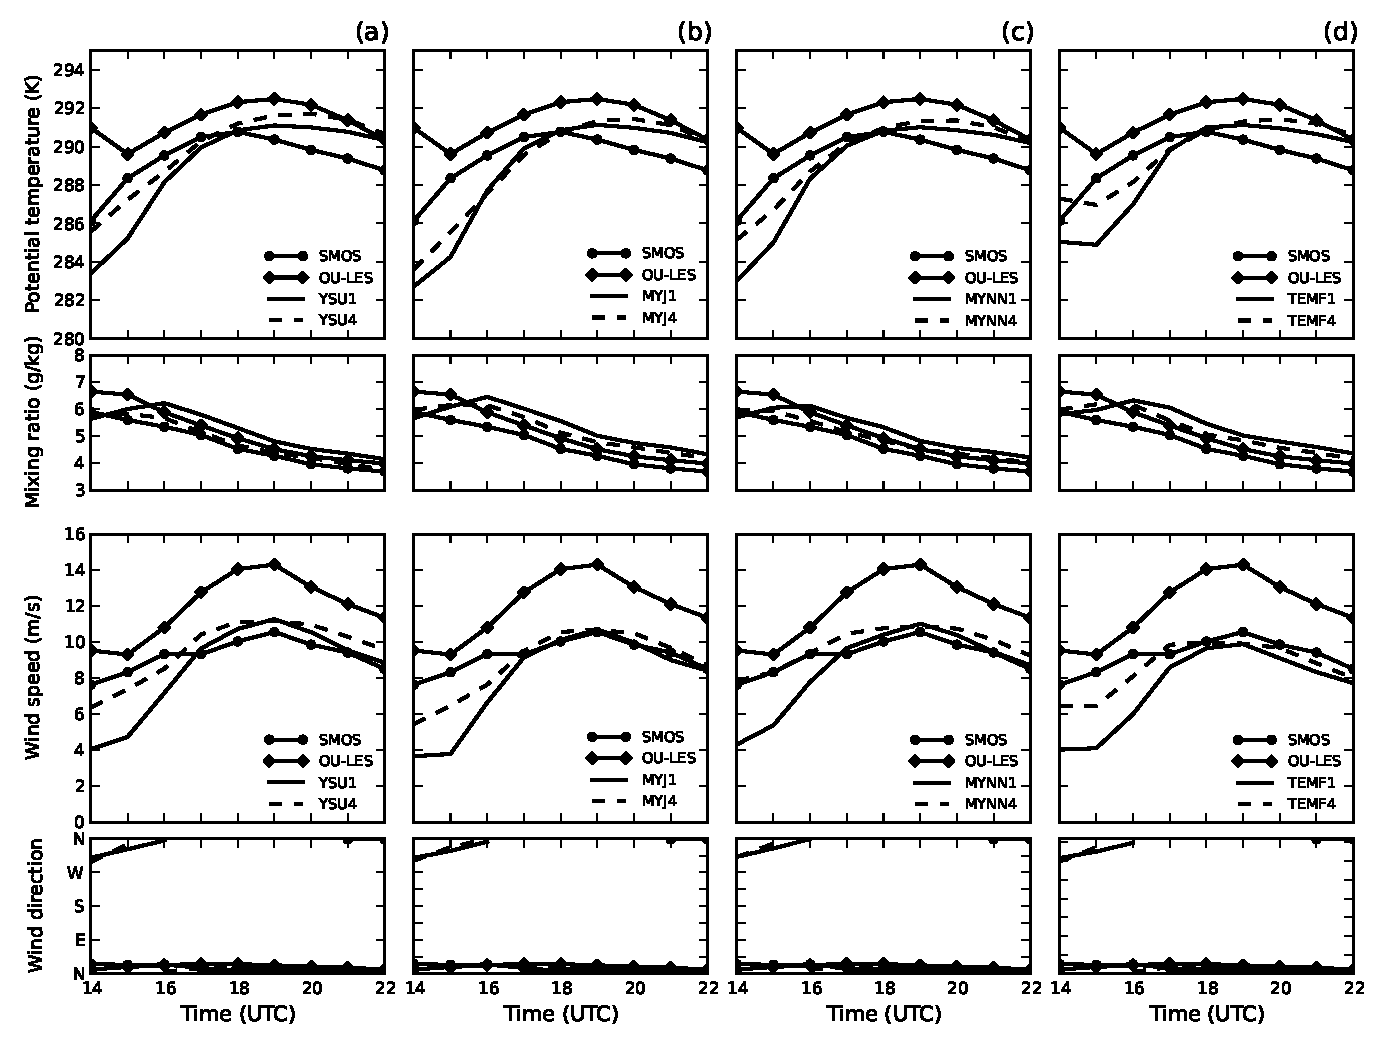
\includegraphics[width=\textwidth]{figures/chapter4/meteogram_grid_20081026}
\end{center}
\caption{Evolution of potential temperature (top row), water vapor mixing ratio (second row), wind speed (third row), and wind direction(bottom row) predicted by the WRF model with (left to right) different parameterization schemes and different grid spacings (denoted by the number after the scheme label in the keys) for 26 October 2008. Observational (SMOS) and OU-LES data are also shown for comparison.}
\label{figure420}
\end{figure}


Comparison of model flux predictions with Lamont observations again yielded notable disparities. Surface sensible heat flux values predicted by the WRF model were lower as compared with the observed values through the first three-fourths of the simulation period. After this time, the WRF model predictions surpassed those observed at Lamont. This behavior was caused by a temporal lag in the evolution of flux by the WRF model. Surface latent heat flux values were grossly overestimated at peak convection time, though they were smaller for a brief period at the beginning of the simulation. The time traces also indicate a temporal shift in the WRF model predictions. Differences between model predictions with disparate grid spacing were rather small and inconsequential (hence, the corresponding data are not shown). 

Figure~\ref{figure421} illustrates the effects of changing grid spacing on turbulence parameters among the four investigated WRF model PBL schemes. Time evolution of $u_*$ predictions from the WRF model did not particularly match phase with observations until the second half of the simulation period. Generally speaking, WRF model predictions were closer to observed values than those from OU-LES data. Each configuration underpredicts values for friction velocity for the first one-third of the day, after which every scheme except the TEMF approach overpredicts values by a considerable amount. The temporal evolution of $\theta_*$ predictions closely matches the phase of the observational time trace. Every scheme matches closely with OU-LES predictions, but underpredicts the magnitude as compared with observations. In general, refined grid spacing in this particular case led to inconsequential improvements to model predictions of both $u_*$ and $\theta_*$. 


\begin{figure}[ht!]
\begin{center}
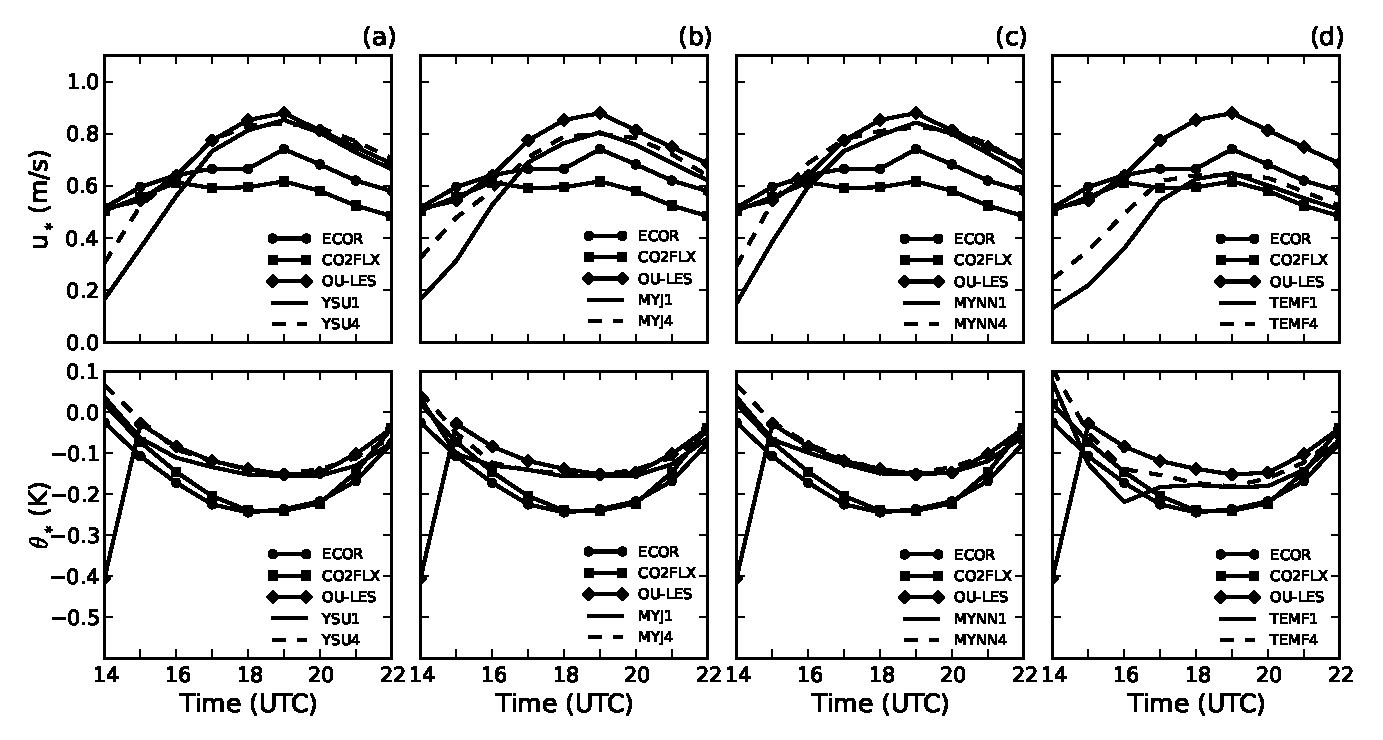
\includegraphics[width=\textwidth]{figures/chapter4/ust_tst_grid_20081026}
\end{center}
\caption{Evolution of (top) friction velocity $u_*$ and (bottom) temperature scale $\theta_*$ predicted by the WRF model with (left to right) different parameterization schemes and different grid spacings (denoted by the number after the scheme label in the keys) for 26 October 2008. Observational (ECOR and CO2FLX) and OU-LES data are also shown for comparison.}
\label{figure421}
\end{figure}


Values for PBL depth estimates were smaller for all WRF model configurations early in the simulation window as compared with OU-LES data. As the CBL developed, the depth estimates from the WRF model closely matched the temporal evolution depicted in OU-LES predictions. With only one available observation point in the simulation period, it is difficult to ascertain how well each approach reproduced the CBL growth evolution. Based on that one point, reduction of grid spacing led to more realistic depth estimates. In terms of the stability parameter, all WRF model predictions except the TEMF scheme were generally consistent with OU-LES data and lower than observational values. Here, the TEMF scheme overestimated the value by a wide margin when contrasted with other WRF model configurations, but was generally consistent with comparison data for the time of peak convection. Differences between WRF model predictions with varying grid spacing were particularly small (the corresponding data are not shown). 

Figure~\ref{figure422} illustrates a meteogram (timeline trace) of basic meteorological variables derived from WRF model output, OU-LES data, and measurements at the Lamont site. Recalling that the 14 UTC values from WRF model represent conditions achieved after 12-hour spin-up, while OU-LES is initialized with local 14 UTC profiles retrieved from the RUC data, all employed SL\slash PBL schemes in the WRF model predict cooler and drier atmospheric conditions as compared with the observed temperature and water vapor mixing ratio. Such characteristics were discovered in the all other investigated CBL cases. The OU-LES data better match the diurnal trends for these fields. For potential temperature, there is little difference between schemes, while for water vapor the YSU scheme predicts values closest to observational and OU-LES data. Wind speed and direction estimates were noticeably different than observations and OU-LES predictions for all schemes in the WRF model over the first one-third of the simulation period. After this time, wind speed and direction predictions with different schemes are rather close to each other, with MYJ and MYNN schemes producing results slightly closer to observations than the YSU and TEMF schemes. Speed values predicted from the WRF model match more closely to observational data, whereas OU-LES values were too large.


\begin{figure}[ht!]
\begin{center}
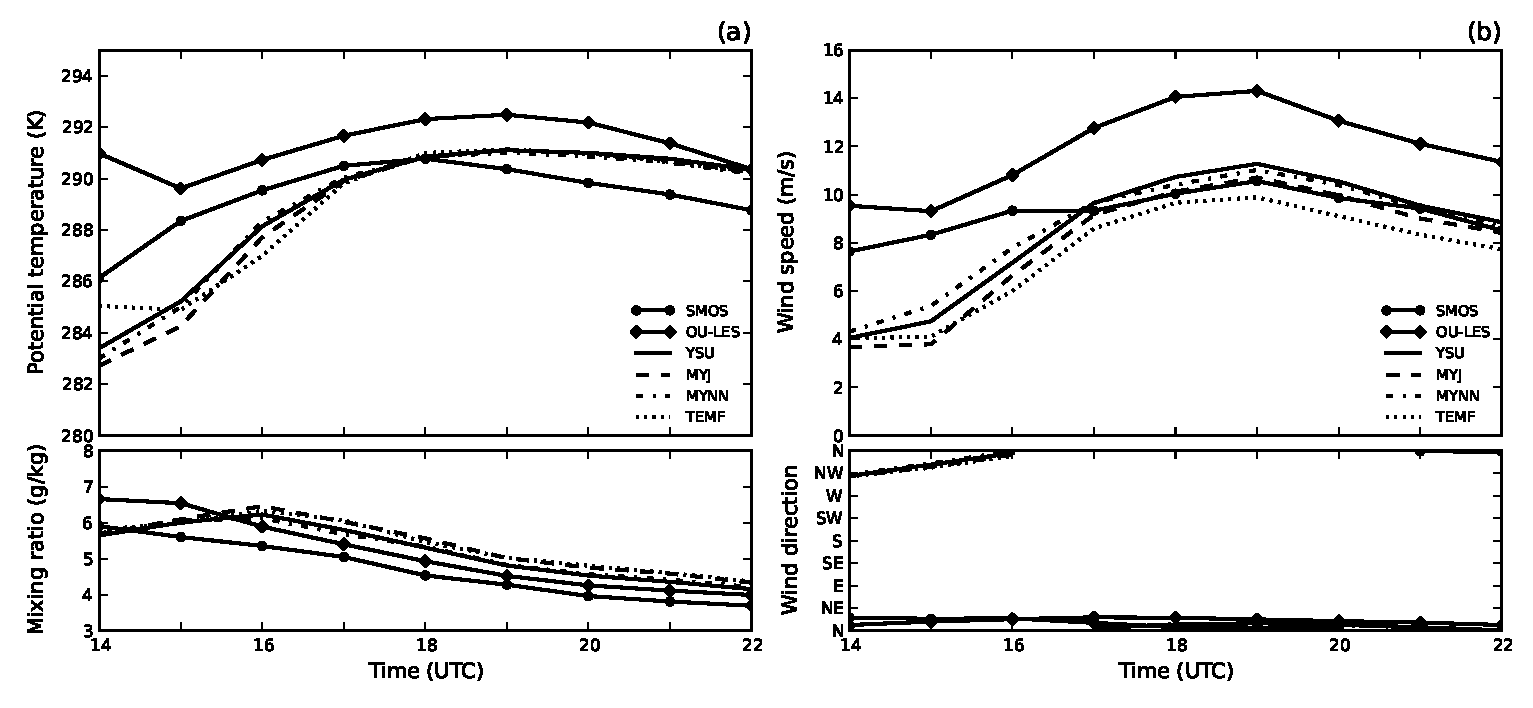
\includegraphics[width=\textwidth]{figures/chapter4/meteogram_phys_20081026}
\end{center}
\caption{Evolution of (a) potential temperature (upper panel) and water vapor mixing ratio (lower panel) and (b) wind speed (upper panel) and wind direction (lower panel) predicted by the WRF model with different parameterization schemes for 26 October 2008. Observational (SMOS) and OU-LES data are also shown for comparison.}
\label{figure422}
\end{figure}


Differences between WRF model predictions and observational heat-flux data are evident in Fig.~\ref{figure423}, though less dramatic than the previously studied CBL cases. Surface sensible heat flux values predicted by the WRF model were lower as compared with the observed values through the first three-fourths of the simulation period. After this time, WRF model predictions surpassed those observed at Lamont. This behavior was caused by a temporal lag in the evolution of flux by the WRF model. Latent heat flux time traces exhibited similar behavior, but with more pronounced differences. Examination of the total heat flux shows that several schemes are consistent with observations, with the YSU approach matching most closely. However, the traces are marked by a temporal lag of $30$ minutes to one hour. For sensible heat flux the YSU scheme is closest to observations than the other three options. For latent heat flux, the YSU scheme is closest overall to observed values during peak convective hours, while the TEMF scheme is by far the most disparate. 


\begin{figure}[ht!]
\begin{center}
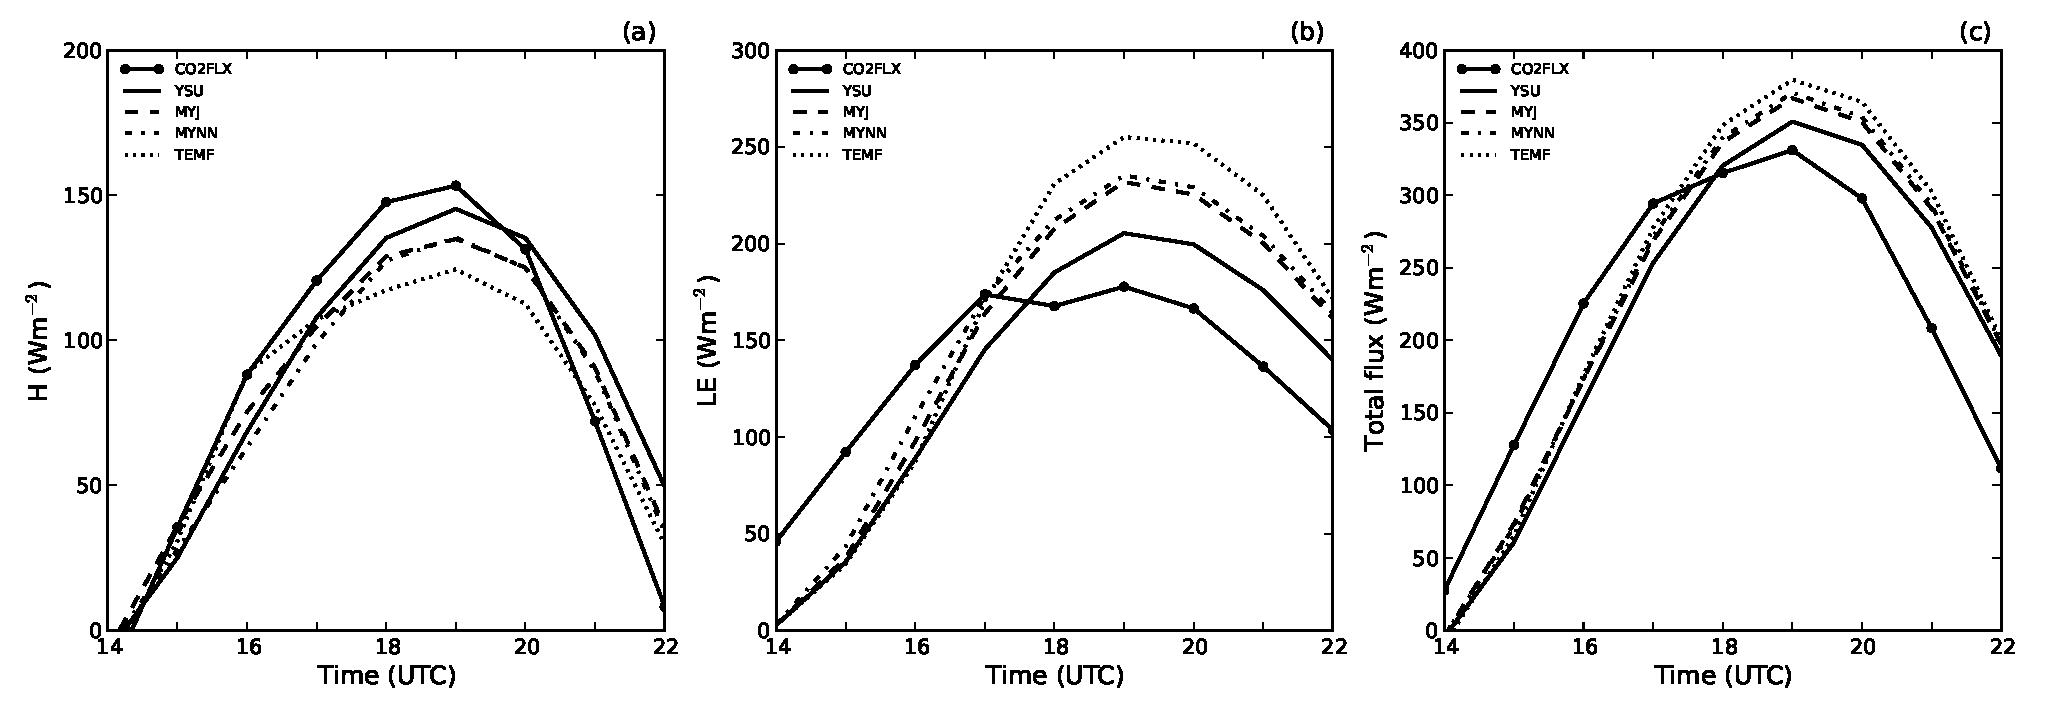
\includegraphics[width=\textwidth]{figures/chapter4/shf_lhf_phys_20081026}
\end{center}
\caption{Evolution of the near-surface (a) sensible, (b) latent, and (c) total heat fluxes predicted by the WRF model with different parameterization schemes for 26 October 2008. Observational data (ECOR and CO2FLX) are also shown for comparison.}
\label{figure423}
\end{figure}


Turbulence scales for velocity and temperature are shown on Fig.~\ref{figure424}. The OU-LES code produces $u_*$ values that are generally consistent with observed data for the first one-third of the simulation period, while those from the WRF model were markedly underpredicted. After this time, OU-LES data and every configuration except the TEMF scheme overpredicts values by a considerable amount, thus exaggerating the mechanical turbulence generation. For times of most active convection, the TEMF and MYJ schemes compare most favorably to observations. The magnitude of the turbulence temperature scale is underestimated for all schemes and is consistent with time traces of OU-LES data. In this regard, the TEMF scheme produces the more accurate result, while few differences exist between the remaining schemes. Such behavior of the modeled $\theta_*$ is consistent with each scheme's respective representation of friction velocity and surface sensible heat flux.


\begin{figure}[ht!]
\begin{center}
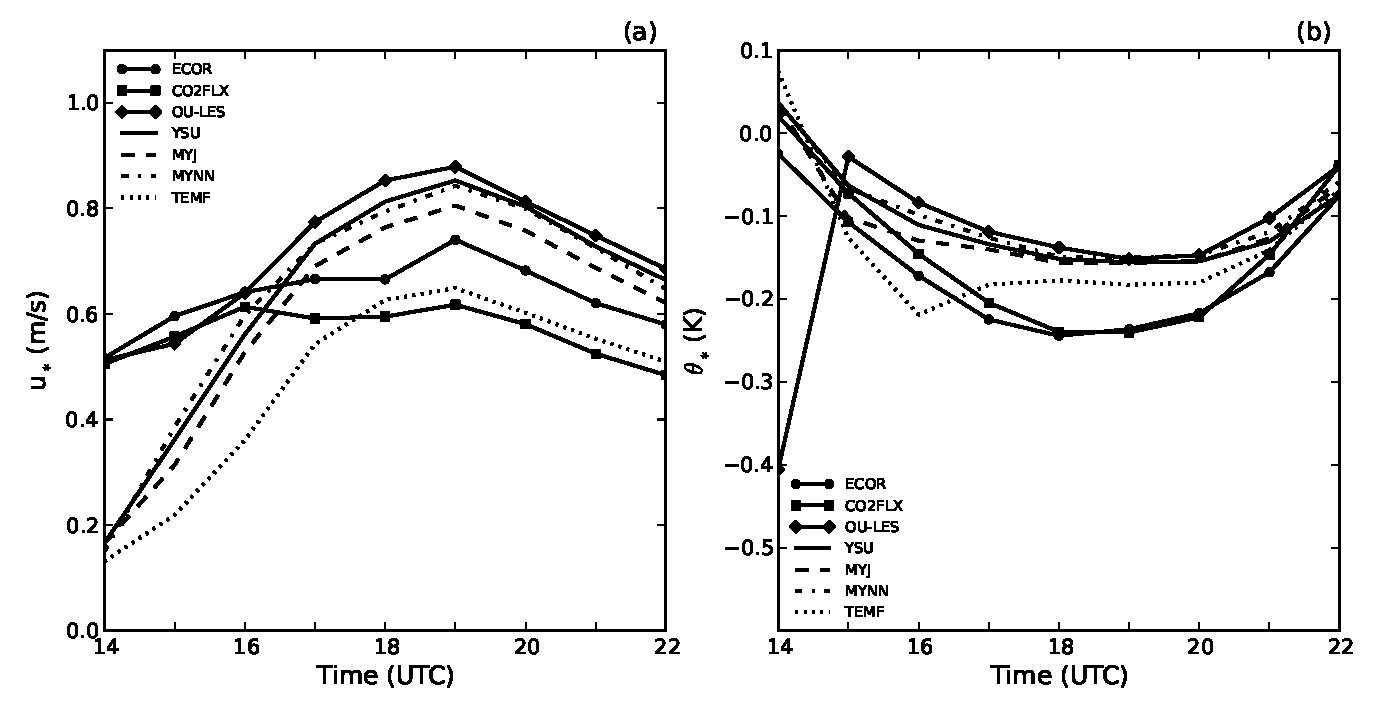
\includegraphics[width=\textwidth]{figures/chapter4/ust_tst_phys_20081026}
\end{center}
\caption{Evolution of the (a) friction velocity $u_*$ and (b) temperature scale $\theta_*$ predicted by the WRF model with different parameterization schemes for 26 October 2008. Observational data (ECOR and CO2FLX) and OU-LES data are also shown for comparison.}
\label{figure424}
\end{figure}


Figure~\ref{figure425} contains one observational value for which to compare against, so statements regarding accuracy must remain conservative. Values for PBL depth estimates were lower for all WRF model configurations early in the simulation window as compared with OU-LES data. As the CBL developed, the depth estimates from the WRF model closely matched the temporal evolution of the OU-LES predictions. Based on available observational data, OU-LES produced the more realistic depth estimates when compared against those from the WRF model. Differences among predictions are largely indistinguishable during times of active convection. In terms of the stability parameter, $\zeta = -z_i / L$, all WRF model predictions except the TEMF scheme were generally consistent with OU-LES data and lower as compared with Lamont observations. Here, the TEMF scheme produced larger values when contrasted with other WRF model PBL schemes, but was generally consistent with comparison data.

Unlike the previously considered CBL cases, the TEMF scheme performed more admirably, especially in terms of turbulence parameters and the representation of CBL development. compared with that case, which was largely driven by buoyancy forcing, a greater portion of the day's CBL development was attributable to shear production. The TEMF scheme calculates friction velocity based on the surface stress, unrelated to the mixing resulting from mass transport. The surface stress only contains a diffusivity component, while the fluxes that relate to the turbulence temperature scale are composed of both a diffusivity and mass flux component. It may be the case that, under conditions of relatively weak winds and strong buoyancy, the physical model that governs the TEMF scheme is not sufficiently robust. In other words, the assumptions that compose the mass flux approach may overestimate the contributions of buoyancy forcing to boundary layer growth when winds are weak.


\begin{figure}[ht!]
\begin{center}
\includegraphics[width=\textwidth]{figures/chapter4/pblh_phi_phys_20081026}
\end{center}
\caption{Evolution of (a) $z_i$ and (b) stability parameter $-\frac{z_i}{L}$ predicted by the WRF model with different parameterization schemes for 26 October 2008. Observational (LMN, ECOR, and CO2FLX) and OU-LES data are also shown (for unstable conditions only).}
\label{figure425}
\end{figure}


\section{Case 4: February 5, 2009}
\label{feb5-46}

\subsection{Meteorological Conditions}
\label{mc-461}


\begin{figure}[H]
     \begin{center}
%
        \subfigure[5 February 2009 12 UTC]{%
            \label{figure407a}
            \includegraphics[width=0.5\textwidth]{figures/chapter4/ruc_20090205_12_composite}
        }%
        \subfigure[5 February 2009 16 UTC]{%
           \label{figure407b}
           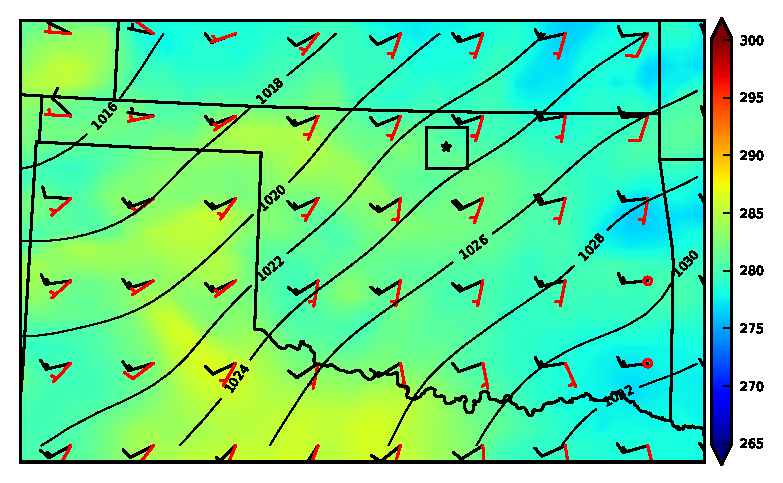
\includegraphics[width=0.5\textwidth]{figures/chapter4/ruc_20090205_16_composite}
        }\\ %  ------- End of the first row ----------------------%
        \subfigure[5 February 2009 20 UTC]{%
            \label{figure407c}
            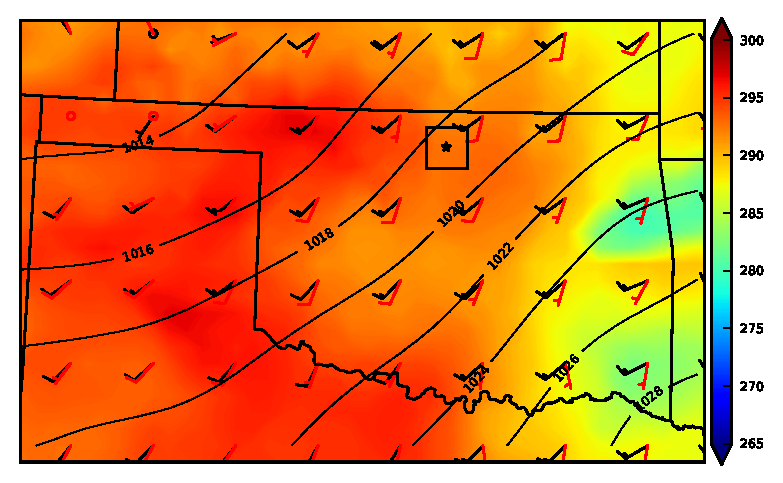
\includegraphics[width=0.5\textwidth]{figures/chapter4/ruc_20090205_20_composite}
        }%
        \subfigure[6 February 2009 00 UTC]{%
            \label{figure407d}
            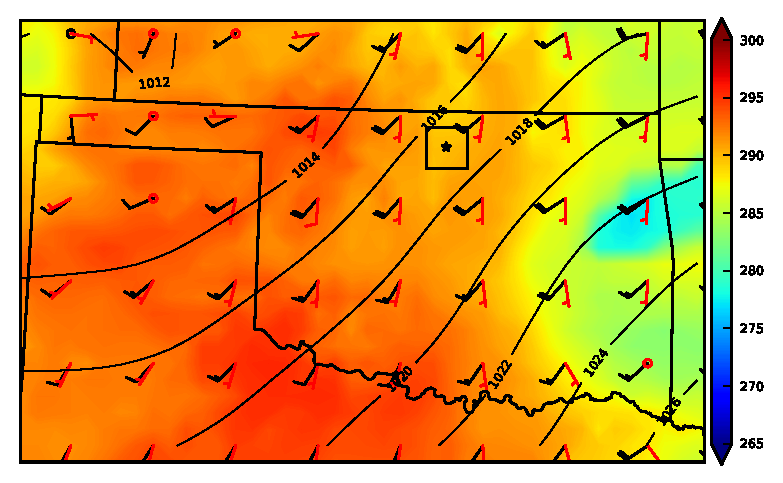
\includegraphics[width=0.5\textwidth]{figures/chapter4/ruc_20090206_00_composite}
        }%
%
    \end{center}
    \caption{%
        Meteorological conditions taken from RUC analyses for 5 February 2009. Surface pressure ($\hecto\pascal$) is the contoured quantity, surface temperature ($\kelvin$) is the shaded quantity, and surface winds and $850\hecto\pascal$ winds ($\metre\reciprocal\second$) are the red and black wind barbs, respectively. The black square represents the comparison domain, while the black star depicts the location of the Lamont, Oklahoma ARM profiler site.}%
   \label{figure426}
\end{figure}


The fourth investigated CBL case was simulated from 1500 UTC (1000 local time) 5 February 2009 to 2200 UTC (1700 local time) 5 February 2009. Unlike other considered CBL cases, clouds were present in the early portion of the simulation period for this date. However, they cleared out within two hours and no precipitation was recorded in the comparison domain. In that sense, the clouds did not corrupt the requirement of a clear and dry CBL case. The CBL was marked with strong wind shear and increasing wind speeds throughout the simulation period. The mixed layer for this case was much shallower than in other considered CBL cases. 

Figure~\ref{figure426} depicts the evolution of meteorological conditions over the geographical region of interest. At the start of the simulation period, a low-pressure center was located in western Kansas. The associated trough was present in the far reaches of the Oklahoma panhandle. Winds at the surface were from the south at $5\mbox{ }\metre\reciprocal\second$ while those at $850\mbox{ }\hecto\pascal$ were from the west-southwest at $15$ to $20\mbox{ }\metre\reciprocal\second$. Accordingly, the CBL was representative of a strong, sheared environment. 

As the day progressed, the low-pressure system deepened to the south-southwest and affected the region of interest. Surface winds shifted slightly to the south-southwest and increased in speed to $10\mbox{ }\metre\reciprocal\second$. Meanwhile, winds at $850\mbox{ }\hecto\pascal$ shifted to the southwest at $15$ to $20\mbox{ }\metre\reciprocal\second$. The effect was a reduction in directional shear and an increase in overall wind speed within the CBL. Surface heating increased during this time, as did the temperature by a relatively substantial amount. 

By the end of the simulation period at 2200 UTC on February 5, 2009, the low-pressure system had further extended into Oklahoma. Surface winds shifted to the south and decreased to $5\mbox{ }\metre\reciprocal\second$. Wind direction at $850\mbox{ }\hecto\pascal$ remained consistent from the southwest at $20\mbox{ }\metre\reciprocal\second$. As a result, the combined effects of directional and speed shear increased within the CBL. Temperatures and moisture, meanwhile, remained fairly constant for several intervening hours. 

Atmospheric soundings at Lamont for 1200, 1800, and 0000 UTC are shown in Fig.~\ref{figure427}. The initial profile of potential temperature showed the expected remnants of a nocturnal inversion, indicative of a strongly stable region near the surface. The low-level moisture profile showed that the environment was much drier than in any of the other studied CBL cases. Surface winds were fairly weak but winds aloft pointed to the presence of a strong south-southwest low-level jet (LLJ). Subsequent profiles of potential temperature illustrated rapid warming and the gradual development of a shallow mixed layer. Mixing ratio profiles indicated a substantial increase in low-level moisture throughout the course of the day. By the end of the simulation period, winds strengthened and the combined effects of speed and directional wind shear increased. This particular CBL case differs from the previously considered cases because the environment had lower temperatures and relatively weak buoyancy forcing as compared with the contribution of mechanical production. These combined effects led to a much shallower mixed layer when compared to the other CBL cases.


\begin{figure}[H]
\begin{center}
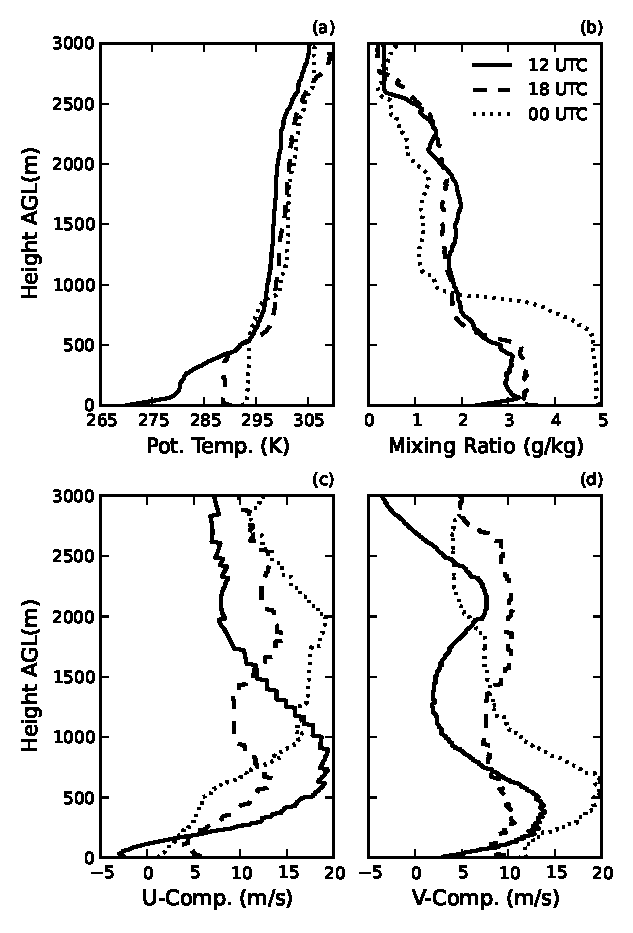
\includegraphics[width=0.5\textwidth]{figures/chapter4/20090205_lmnsounding}
\end{center}
\caption{Atmospheric soundings at the LMN site for 5 February 2009: (a) potential temperature, (b) water vapor mixing ratio, (c) u component of wind, and (d) y component of wind. Solid, dashed, and dotted lines correspond, respectively, to 1200, 1800, and 0000 (following day) UTC.}
\label{figure427}
\end{figure}


\subsection{Results}
\label{res-462}

Figure~\ref{figure428} illustrates the effects of changing grid spacing for potential temperature, water vapor mixing ratio, wind speed, and wind direction. Potential temperature and moisture values were initially lower than observational and OU-LES data, similar to findings in other considered CBL cases. This may likely demonstrate that the WRF model SL\slash PBL parameterization schemes struggle under stable conditions. For all schemes, the WRF model predicted values for potential temperature that were lower than observational and OU-LES data, although the shape of the time evolution matched rather closely. It should be noted that the MYNN scheme used in conjunction with $4$-$\kilo\metre$ grid spacing produced potential temperature values much closer to observations than any other WRF model configuration. For both the potential temperature and mixing ratio, OU-LES time evolution matched the physical trend better than did the WRF model. Differences among model outputs with varying grid spacing values were relatively minor. Model runs using $4$-$\kilo\metre$ spacing compared more favorably with observations for potential temperature than did those using $1$-$\kilo\metre$ spacing, while the opposite was true for water vapor mixing ratio. Modeled horizontal wind speed values were systematically underpredicted with all turbulence scheme and grid spacing combinations. When differences between outputs with disparate grid spacing values were notable, model configurations employing $4$-$\kilo\metre$ spacing more often reproduced values closer to observations. Wind direction estimates were generally consistent between both OU-LES predictions and all scheme\slash spacing combinations in the WRF model, comparing favorably with observations. Variations in grid spacing resulted in rather inconsequential improvements.


\begin{figure}[ht!]
\begin{center}
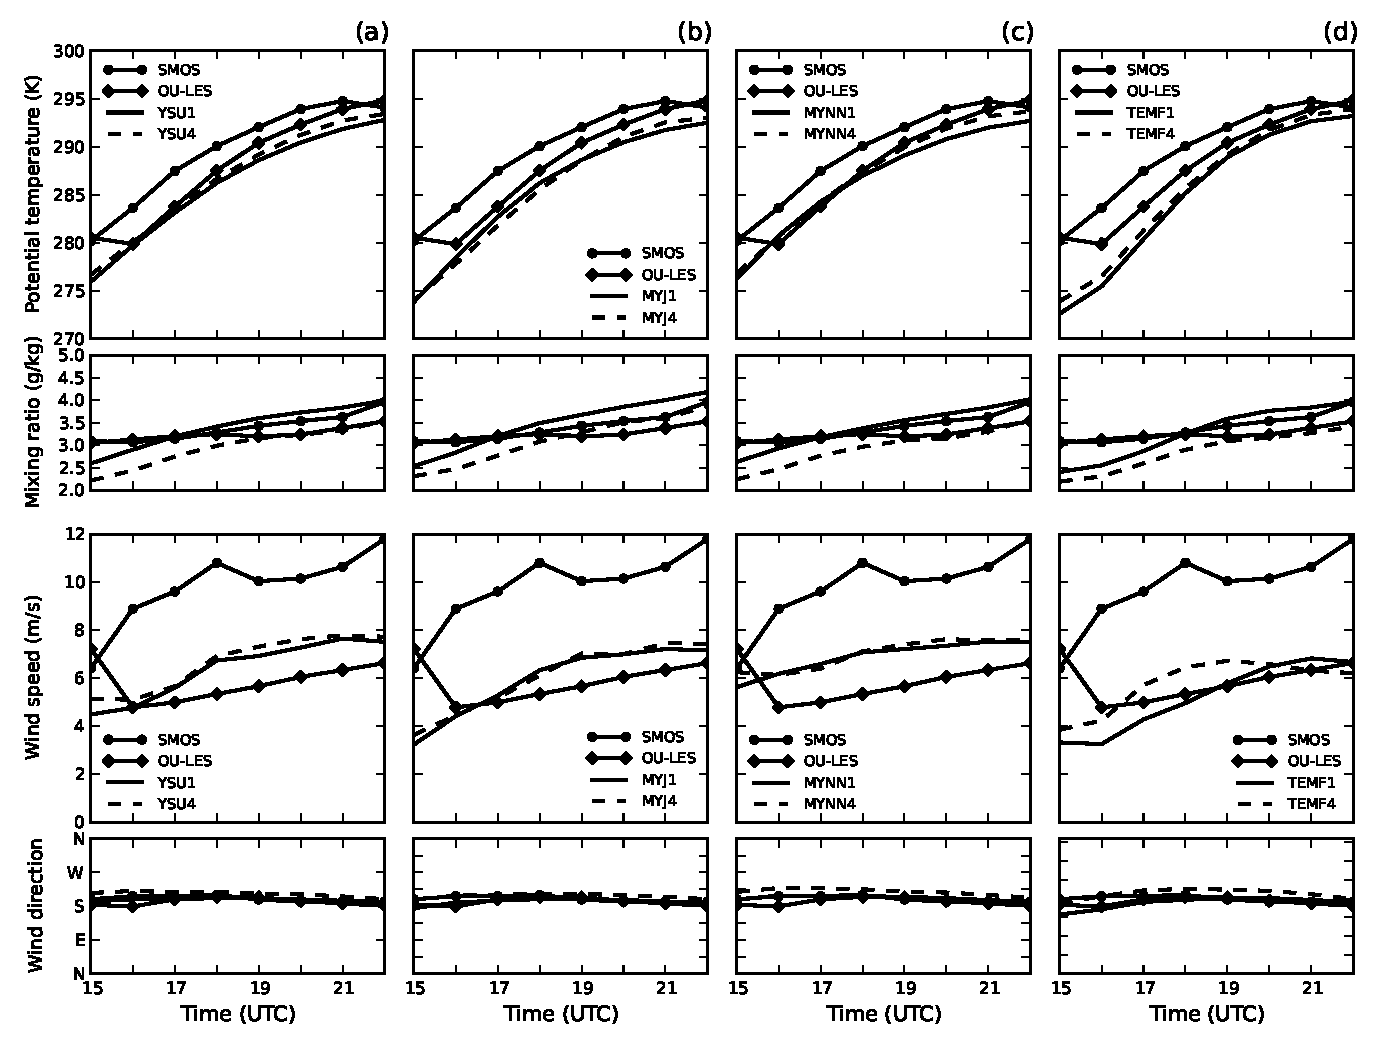
\includegraphics[width=\textwidth]{figures/chapter4/meteogram_grid_20090205}
\end{center}
\caption{Evolution of potential temperature (top row), water vapor mixing ratio (second row), wind speed (third row), and wind direction(bottom row) predicted by the WRF model with (left to right) different parameterization schemes and different grid spacings (denoted by the number after the scheme label in the keys) for 5 February 2009. Observational (SMOS) and OU-LES data are also shown for comparison.}
\label{figure428}
\end{figure}


Comparison of model flux predictions with Lamont observations followed the trends observed in the previously examined CBL cases. Surface sensible heat flux values predicted by the WRF model were generally lower as compared with the observed values. As the exception, predictions from the MYJ and TEMF schemes were larger than observed values for the first one-third of the simulation period. This is indicative of a similar temporal shift as was observed in the previously studied CBL case. Surface latent heat flux values were again appreciably overestimated for the majority of the simulation period. Differences between model predictions with varying grid spacings were rather small and inconsequential (hence, the corresponding data are not shown). 

Figure~\ref{figure429} illustrates the effects of changing grid spacing on turbulence parameters among the four investigated WRF model PBL schemes. Time evolution of $u_*$ predictions from OU-LES data closely matches phase with, and is closer in value to, observational values for the first one-half of the simulation period. After that time, all schemes from the WRF model produce values that better match observational data, with the exception of the TEMF scheme. The temporal evolution of $\theta_*$ predictions matches the phase of the time trace of observations. Every scheme compares closely with observed data and OU-LES predictions, with the lone exception of the TEMF scheme, which grossly overpredicts the magnitude of $\theta_*$. In general, refined grid spacing in this particular case led to inconsequential improvements to model predictions of both $u_*$ and $\theta_*$. 


\begin{figure}[ht!]
\begin{center}
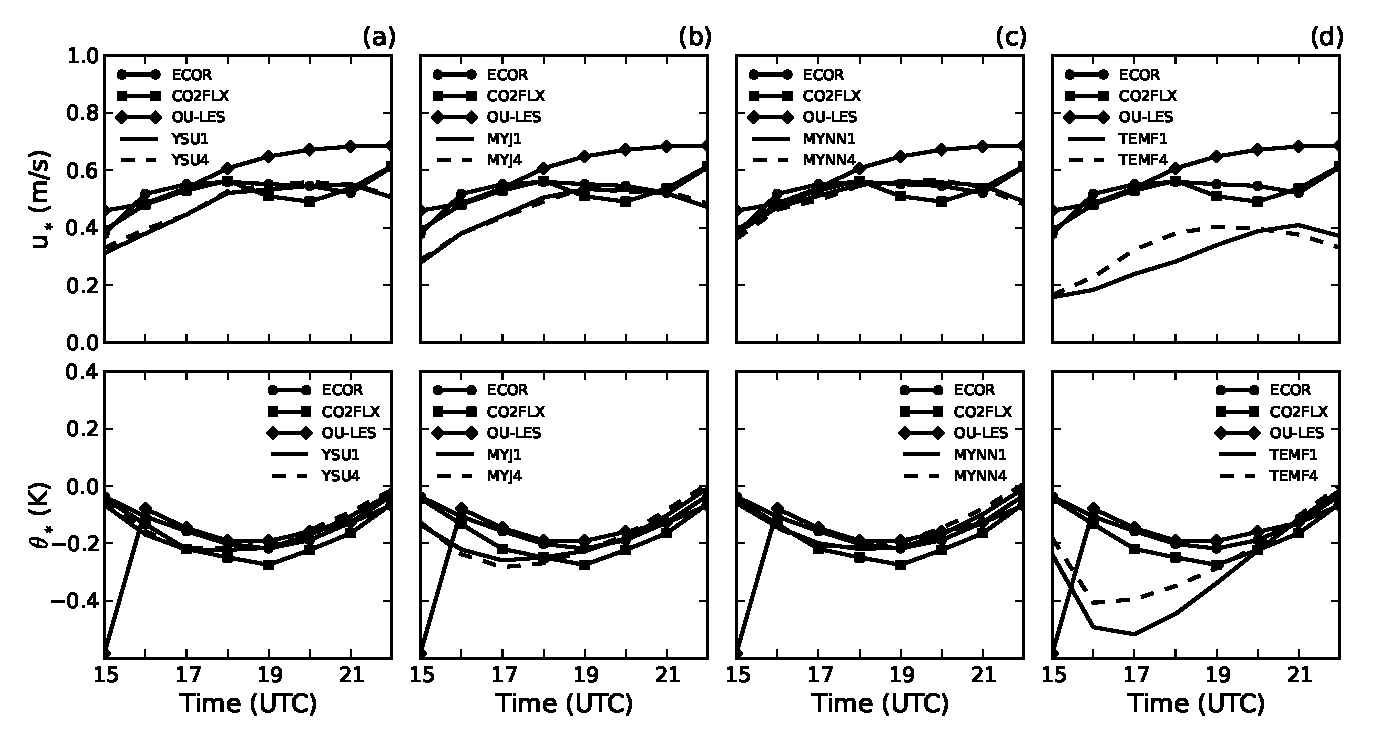
\includegraphics[width=\textwidth]{figures/chapter4/ust_tst_grid_20090205}
\end{center}
\caption{Evolution of (top) friction velocity $u_*$ and (bottom) temperature scale $\theta_*$ predicted by the WRF model with (left to right) different parameterization schemes and different grid spacings (denoted by the number after the scheme label in the keys) for 5 February 2009. Observational (ECOR and CO2FLX) and OU-LES data are also shown for comparison.}
\label{figure429}
\end{figure}


Values for PBL depth estimates were generally consistent for all WRF model configurations early in the simulation window as compared with OU-LES data. The depth estimates from the WRF model became stagnant as the CBL developed, except for the TEMF configuration, which showed similar growth to that of OU-LES data. In all cases, reduction of grid spacing led to more realistic depth estimates. With only one observation time available, it is difficult to surmise how well the stability parameter was predicted throughout the entire simulation time window. However, for the one comparison time, all WRF model predictions except that from the TEMF scheme were generally close to the observational value. Here, the TEMF scheme overestimated the value by a wide margin, which is not surprising given the associated predictions of friction velocity and turbulence temperature scale. Differences between WRF model predictions with varying grid spacing were inconsequential during portions of the day with peak convective activity (the corresponding data are not shown). 

Figure~\ref{figure430} illustrates a meteogram (timeline trace) of basic meteorological variables derived from WRF model output, OU-LES data, and measurements at the Lamont site. Recalling that the 15 UTC values from WRF model represent conditions achieved after 12-hour spin-up, while OU-LES is initialized with local 15 UTC profiles retrieved from the RUC data, one again notes a common problem for employed SL\slash PBL schemes in the WRF model at the beginning of the day: they all predict cooler and drier atmospheric conditions as compared with the observed temperature and water vapor mixing ratio. Such characteristics have been common across all previously considered CBL cases. The OU-LES data better match the diurnal trends for these fields. For potential temperature, the greatest differences between schemes are in the first one-half of the simulation period, where the YSU and MYNN schemes match closer to observational and OU-LES data. After that time, WRF model predictions converge. Wind speed and direction predictions with different schemes are reasonably close to each other, with MYNN and YSU schemes producing results slightly closer to observations than the MYJ and TEMF schemes. Wind speeds from OU-LES are further from observational data than those from the WRF model. Speed values predicted from both approaches are lower than observational data. Again, this may simply illustrate local flow effects that OU-LES and WRF model predictions fail to capture across the entirety of a numerical grid cell.


\begin{figure}[ht!]
\begin{center}
\includegraphics[width=\textwidth]{figures/chapter4/meteogram_phys_20090205}
\end{center}
\caption{Evolution of (a) potential temperature (upper panel) and water vapor mixing ratio (lower panel) and (b) wind speed (upper panel) and wind direction (lower panel) predicted by the WRF model with different parameterization schemes for 5 February 2009. Observational (SMOS) and OU-LES data are also shown for comparison.}
\label{figure430}
\end{figure}


Notable differences between WRF model predictions and observational heat-flux data are evident in Fig.~\ref{figure431}, though such differences are less pronounced than in other investigated cases. Surface sensible heat flux values predicted by the WRF model were generally lower as compared with the observed values. However, predictions from the MYJ and TEMF schemes were overpredicted as compared with observed values for the first one-third of the simulation period. This is indicative of a similar temporal shift that was observed in the previously studied CBL case. Surface latent heat flux values were again appreciably overestimated for the majority of the simulation period, except that no time lag was present. Examination of total flux shows that each scheme was generally consistent with observations, but that the WRF model once again suffers from a partitioning error. For times of peak convection, the MYJ and TEMF schemes most closely match observational values for sensible heat flux. For latent heat flux, the YSU scheme is closest to observed values, while the MYNN scheme is the most disparate. 


\begin{figure}[ht!]
\begin{center}
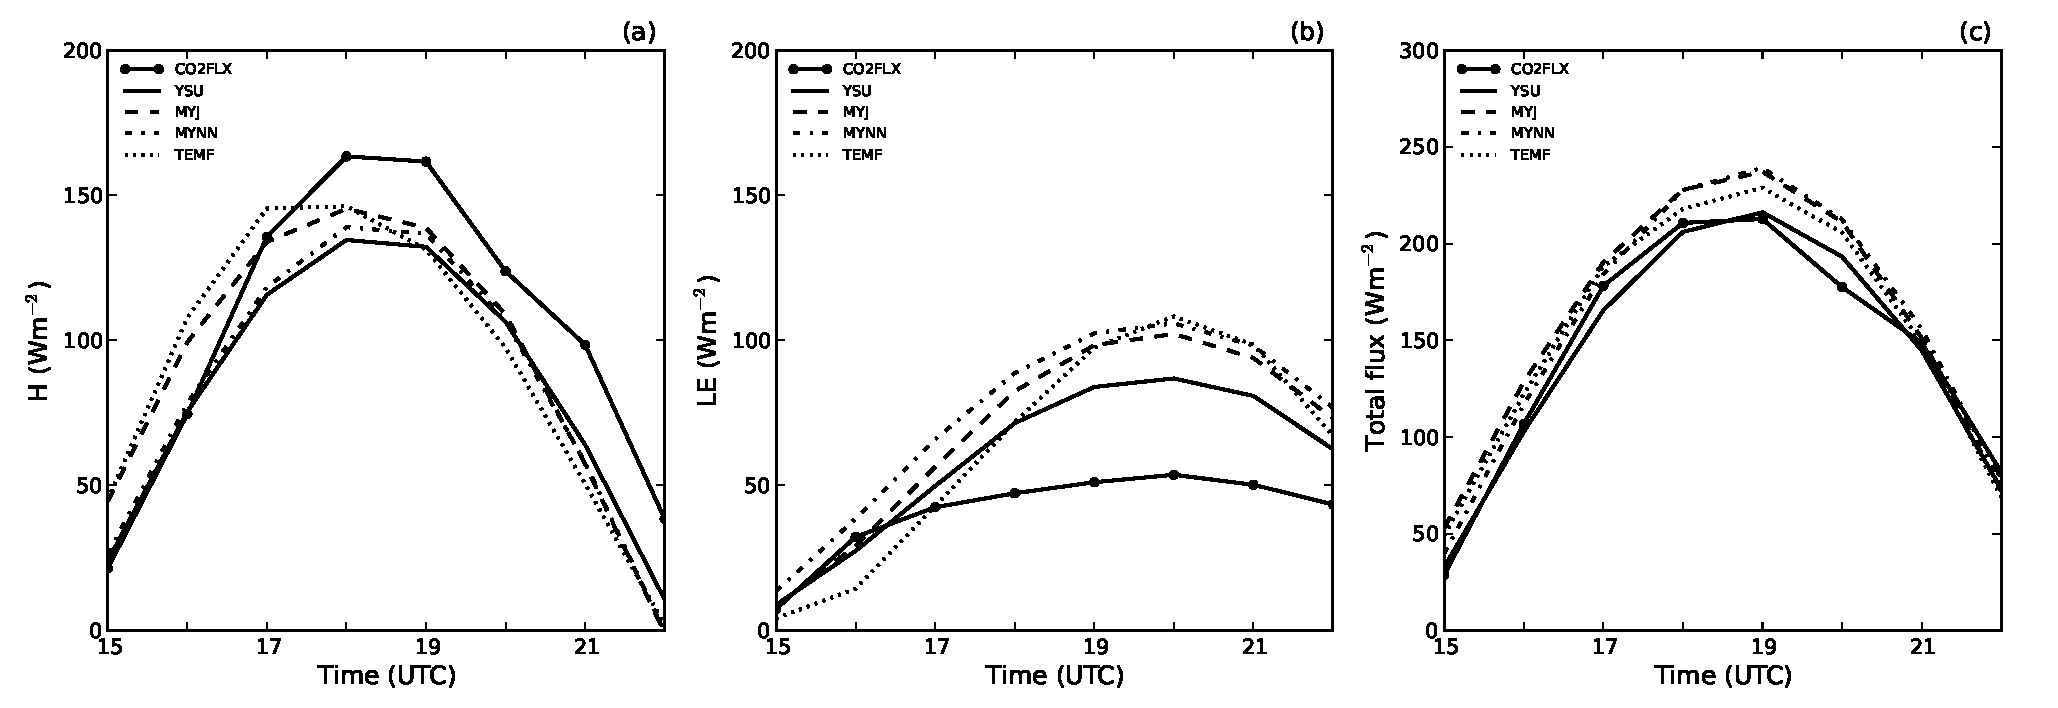
\includegraphics[width=\textwidth]{figures/chapter4/shf_lhf_phys_20090205}
\end{center}
\caption{Evolution of the near-surface (a) sensible, (b) latent, and (c) total heat fluxes predicted by the WRF model with different parameterization schemes for 5 February 2009. Observational data (ECOR and CO2FLX) are also shown for comparison.}
\label{figure431}
\end{figure}


Turbulence scales for velocity and temperature are shown in Fig.~\ref{figure432}. Time evolution of $u_*$ predictions from OU-LES data closely matches phase with, and is closer in value to, observational values for the first one-half of the simulation period. After that time, all schemes from the WRF model produce values that better match observational data, with the exception of the TEMF scheme. The MYNN scheme compares most favorably to observations, while the TEMF scheme predicts values that are significantly lower. The magnitude of the turbulence temperature scale is confidently reproduced by the OU-LES code and all WRF model configurations, except for the TEMF scheme, which grossly overpredicts the magnitude of $\theta_*$. Such behavior of the modeled $\theta_*$ is consistent with each scheme's respective underprediction of friction velocity and surface sensible heat flux.


\begin{figure}[ht!]
\begin{center}
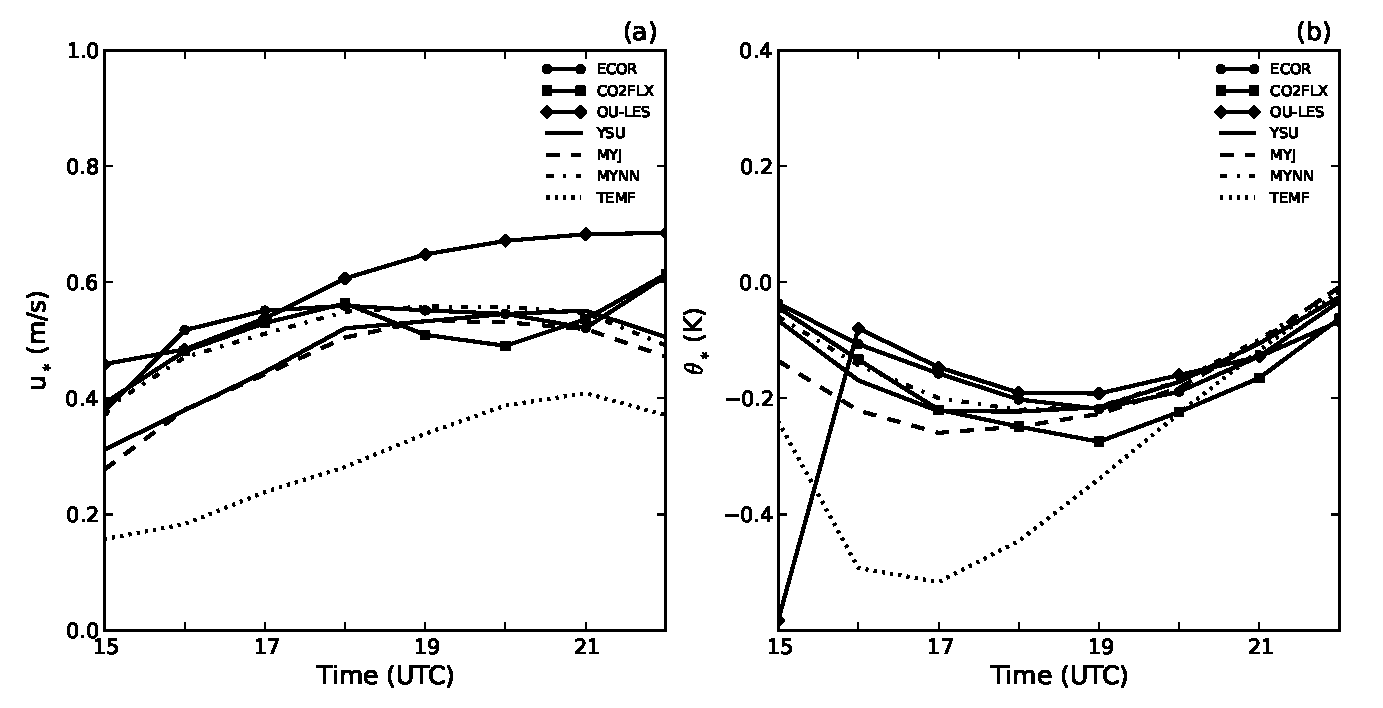
\includegraphics[width=\textwidth]{figures/chapter4/ust_tst_phys_20090205}
\end{center}
\caption{Evolution of the (a) friction velocity $u_*$ and (b) temperature scale $\theta_*$ predicted by the WRF model with different parameterization schemes for 5 February 2009. Observational data (ECOR and CO2FLX) and OU-LES data are also shown for comparison.}
\label{figure432}
\end{figure}


Values for PBL depth estimates, shown in Fig.~\ref{figure433}, were generally consistent for all WRF model configurations early in the simulation window as compared with OU-LES data. Values for every approach match closely with observational data. For the stability parameter, $\zeta = -z_i / L$, the YSU, MYJ, and MYNN schemes produce values closest to the OU-LES data for times of peak convective activity. Oppositely, the TEMF values are significantly larger, undoubtedly a result of significant underprediction of shear forcing and overprediction of buoyancy forcing in the CBL development. Compared to WRF model predictions, the OU-LES attributes slightly more shear forcing to the CBL development.


\begin{figure}[ht!]
\begin{center}
\includegraphics[width=\textwidth]{figures/chapter4/pblh_phi_phys_20090205}
\end{center}
\caption{Evolution of (a) $z_i$ and (b) stability parameter $-\frac{z_i}{L}$ predicted by the WRF model with different parameterization schemes for 5 February 2009. Observational (LMN, ECOR, and CO2FLX) and OU-LES data are also shown (for unstable conditions only).}
\label{figure433}
\end{figure}


\section{Case 5: May 31, 2009}
\label{may31-47}

\subsection{Meteorological Conditions}
\label{mc-471}


\begin{figure}[H]
     \begin{center}
%
        \subfigure[31 May 2009 12 UTC]{%
            \label{figure409a}
            \includegraphics[width=0.5\textwidth]{figures/chapter4/ruc_20090531_12_composite}
        }%
        \subfigure[31 May 2009 16 UTC]{%
           \label{figure409b}
           \includegraphics[width=0.5\textwidth]{figures/chapter4/ruc_20090531_16_composite}
        }\\ %  ------- End of the first row ----------------------%
        \subfigure[31 May 2009 20 UTC]{%
            \label{figure409c}
            \includegraphics[width=0.5\textwidth]{figures/chapter4/ruc_20090531_20_composite}
        }%
        \subfigure[1 June 2009 00 UTC]{%
            \label{figure409d}
            \includegraphics[width=0.5\textwidth]{figures/chapter4/ruc_20090601_00_composite}
        }%
%
    \end{center}
    \caption{%
        Meteorological conditions taken from RUC analyses for 31 May 2009. Surface pressure ($\hecto\pascal$) is the contoured quantity, surface temperature ($\kelvin$) is the shaded quantity, and surface winds and $850\hecto\pascal$ winds ($\metre\reciprocal\second$) are the red and black wind barbs, respectively. The black square represents the comparison domain, while the black star depicts the location of the Lamont, Oklahoma ARM profiler site.}%
   \label{figure434}
\end{figure}


The final investigated CBL case was simulated from 1300 UTC (0800 local time) 31 May 2009 to 2300 UTC (1800 local time) 31 May 2009, representing a broad time range of convective conditions. Clouds were again absent during the simulation period. However, storms developed after the time of interest. In that sense, one may consider the CBL in this case a pre-storm environment. The absence of clouds allowed for strong surface heating and was accompanied by small shifts in wind direction, while wind speeds remained fairly unchanged. As a consequence, a deep CBL developed during the course of the day, driven primarily by active buoyancy forcing. 

Figure~\ref{figure434} shows the evolution of meteorological conditions for the region of interest. At the start of the simulation period, a surface low-pressure center was established in the far northwest corner of the Oklahoma panhandle, with a trough extending southward into west Texas. Surface winds were light and from the south-southeast while those at $850\mbox{ }\hecto\pascal$ were from the southwest at $5$ to $15\mbox{ }\metre\reciprocal\second$. The CBL was consistent with conditions of weak to moderate shear. 

As the day progressed, the low-pressure center and associated trough moved eastward toward the comparison domain and into the Texas and Oklahoma panhandles. Surface winds veered to the south-southwest and remained relatively weak at $5\mbox{ }\metre\reciprocal\second$. Winds at $850\mbox{ }\hecto\pascal$ shifted slightly to the south-southwest and reduced to $5\mbox{ }\metre\reciprocal\second$. Accordingly, effects of shear in the CBL were relatively weak during this time. Surface heating was strong and temperatures actively increased. 

By the end of the simulation period at 2300 UTC on May 31, 2009, the low-pressure system pushed further into Oklahoma. Surface winds backed slightly to the south and south-southwest and remained in the range of $5\mbox{ }\metre\reciprocal\second$, while winds at $850\mbox{ }\hecto\pascal$ backed slightly to the south at $10\mbox{ }\metre\reciprocal\second$. As a result, increased speed and directional wind shear contributions were small but measurable. Temperatures and moisture also began to decrease during this period.

Figure~\ref{figure435} shows soundings at Lamont for 1200, 1800, and 0000 UTC. The initial profile of potential temperature depicted a stably-stratified near-surface layer associated with a nocturnal inversion. There was a shallow peak in near-surface moisture as indicated in the mixing ratio profile. Surface winds were fairly weak, while peak values for wind speed were found at $500\mbox{ }\metre$ AGL, resulting in moderate low-level shear. As time progressed, sounding data showed rapid warming and active mixing throughout the CBL. This mixing resulted in a modest reduction in moisture. Velocity components shifted toward the south, reduced in speed, and were actively mixed within the CBL. Accordingly, the effects of shear forcing on CBL growth was reduced throughout the period, while buoyancy forcing dominated. As compared with other studied cases, this CBL was indicative of an environment with strong surface heating, weak but measurable mean winds, and buoyancy forcing that led to a deep, well-mixed layer. Storms were present following the simulation period, meaning the considered CBL may be viewed as a pre-storm environment. 


\begin{figure}[H]
\begin{center}
\includegraphics[width=0.5\textwidth]{figures/chapter4/20090531_lmnsounding}
\end{center}
\caption{Atmospheric soundings at the LMN site for 31 May 2009: (a) potential temperature, (b) water vapor mixing ratio, (c) u component of wind, and (d) y component of wind. Solid, dashed, and dotted lines correspond, respectively, to 1200, 1800, and 0000 (following day) UTC.}
\label{figure435}
\end{figure}


\subsection{Results}
\label{res-472}

Figure~\ref{figure436} illustrates the effects of changing grid spacing for potential temperature, water vapor mixing ratio, wind speed, and wind direction. Unlike the previous four studied CBL cases, potential temperature values matched closely with those recorded by observations. However, moisture values remained comparatively low at the beginning of the simulation window as compared with observational and OU-LES data. Apparently, the employed PBL schemes in the WRF model still struggle to properly handle stable conditions for moisture. For all schemes, the WRF model predicted values for potential temperature that were equivalent to those from observational and OU-LES data. The shape of the time evolution matched exceptionally well. Much like the February 5, 2009 CBL case, the TEMF scheme used in conjunction with $4$-$\kilo\metre$ grid spacing produced potential temperature values much closer to observations than any other WRF model configuration. For both the potential temperature and mixing ratio, OU-LES time evolution matched the physical trend equally close as did the WRF model. Differences among model outputs with varying grid spacing values were minor. Model runs using $4$-$\kilo\metre$ spacing compared equally well with observations for potential temperature and water vapor mixing ratio as did those using $1$-$\kilo\metre$ spacing. Horizontal wind speed values were generally underpredicted with all turbulence scheme and grid spacing combinations. When differences between outputs with disparate grid spacing values were notable, no particular parameterization combination was preferred in regards to comparisons with observations. Wind direction estimates were nearly identical to observations for both OU-LES predictions and all scheme\slash spacing combinations in the WRF model. Any differences may illustrate a scenario in which local conditions at the observing site were different than the mean value across the model grid cell. Variations in grid spacing resulted in rather inconsequential improvements.


\begin{figure}[ht!]
\begin{center}
\includegraphics[width=\textwidth]{figures/chapter4/meteogram_grid_20090531}
\end{center}
\caption{Evolution of potential temperature (top row), water vapor mixing ratio (second row), wind speed (third row), and wind direction(bottom row) predicted by the WRF model with (left to right) different parameterization schemes and different grid spacings (denoted by the number after the scheme label in the keys) for 31 May 2009. Observational (SMOS) and OU-LES data are also shown for comparison.}
\label{figure436}
\end{figure}


Comparison of model flux predictions with Lamont observations again mirrored previously observed behavior. Surface sensible heat flux values predicted by the WRF model were lower as compared to the observed values through the first one-half of the simulation period. After this time, WRF model predictions surpassed those observed at Lamont. This behavior is indicative of a temporal lag in the time trace of flux by the WRF model. Surface latent heat flux values were grossly overestimated at peak convective time, though they matched rather closely for a brief period at the beginning of the simulation. The time traces are devoid of a temporal shift in the WRF model predictions. Differences between model predictions with disparate grid spacing were rather small and inconsequential (hence, the corresponding data are not shown). 

Figure~\ref{figure437} illustrates the effects of changing grid spacing on turbulence parameters among the four investigated WRF model PBL schemes. Time evolution of $u_*$ predictions from all WRF model configurations reasonably matches phase with observations and equally departs from observed values as those in OU-LES data. Each configuration overpredicts values for friction velocity, except those from the TEMF scheme, which are significantly lower than observed data. The temporal evolution of $\theta_*$ predictions matches the phase of the time trace of observations. Every scheme compares closely with observed data and OU-LES predictions, with the lone exception of the TEMF scheme, which grossly overpredicts the magnitude of $\theta_*$ over the last two-thirds of the simulation period. In general, refined grid spacing in this particular case led to inconsequential improvements to model predictions of both $u_*$ and $\theta_*$. 


\begin{figure}[ht!]
\begin{center}
\includegraphics[width=\textwidth]{figures/chapter4/ust_tst_grid_20090531}
\end{center}
\caption{Evolution of (top) friction velocity $u_*$ and (bottom) temperature scale $\theta_*$ predicted by the WRF model with (left to right) different parameterization schemes and different grid spacings (denoted by the number after the scheme label in the keys) for 31 May 2009. Observational (ECOR and CO2FLX) and OU-LES data are also shown for comparison.}
\label{figure437}
\end{figure}


As the CBL increased, the PBL depth estimates from the WRF model grew too quickly and those from OU-LES grew too slowly. With only one observation time available, it is difficult to surmise how well the stability parameter was predicted throughout the entire simulation time window. However, for the one comparison time, all WRF model predictions except the TEMF scheme were generally close to the observational value. Here, the TEMF scheme overestimated the value by a wide margin, which is not surprising given the associated predictions of friction velocity and turbulence temperature scale. Differences between WRF model predictions with varying grid spacing were inconsequential during portions of the day with peak convective activity (the corresponding data are not shown). 

Figure~\ref{figure438} illustrates a meteogram (timeline trace) of basic meteorological variables derived from WRF model output, OU-LES data, and measurements at the Lamont site. However, moisture values remained comparatively low at the beginning of the simulation period as compared with observational and OU-LES data. Predictions from the WRF model better match the diurnal trend from observational potential temperature values, while OU-LES data better match the diurnal trends for moisture. For potential temperature and moisture, differences between schemes are small. Wind speed and direction predictions with different schemes match closely to each other, except at the beginning portion of the simulation period. At that time, the MYNN and YSU schemes produce results slightly closer to observations than the MYJ and TEMF schemes. For the remainder of the day, values predicted from the WRF model configurations converge. Wind speeds from OU-LES are further from observational data than those from the WRF model. Speed values predicted from both approaches are lower than observational data. This consistent underprediction of near-surface wind may indicate that local effects at the measurement site are not captured across the entire model grid cell.


\begin{figure}[ht!]
\begin{center}
\includegraphics[width=\textwidth]{figures/chapter4/meteogram_phys_20090531}
\end{center}
\caption{Evolution of (a) potential temperature (top panel) and water vapor mixing ratio (lower panel) and (b) wind speed (top panel) and wind direction (lower panel) predicted by the WRF model with different parameterization schemes for 31 May 2009. Observational (SMOS) and OU-LES data are also shown for comparison.}
\label{figure438}
\end{figure}


Fig.~\ref{figure439} shows the comparison of model flux predictions with Lamont observations, which again mirrors previously investigated behavior. Surface sensible heat flux values predicted by the WRF model were lower as compared to the observed values through the first one-half of the simulation period. After this time, WRF model predictions surpassed those observed at Lamont due to temporal lag in the time trace of flux by the WRF model. Surface latent heat flux values were grossly overestimated at peak convection time, though they matched rather closely for a brief period at the beginning of the simulation. The time traces showed no evidence of a temporal shift in the WRF model predictions. It is unclear if these differences are proof of an internal partitioning problem within the WRF model, or whether local effects are not representative of the entire grid cell. For times of peak convection, the YSU scheme is closest to observations of sensible heat flux than the other three options. For latent heat flux, the YSU, MYJ, and MYNN scheme compare equally well with observations, while the TEMF scheme is the most disparate. 


\begin{figure}[ht!]
\begin{center}
\includegraphics[width=\textwidth]{figures/chapter4/shf_lhf_phys_20090531}
\end{center}
\caption{Evolution of the near-surface (a) sensible, (b) latent, and (c) total heat fluxes predicted by the WRF model with different parameterization schemes for 31 May 2009. Observational data (ECOR and CO2FLX) are also shown for comparison.}
\label{figure439}
\end{figure}


Turbulence scales for velocity and temperature are shown in Fig.~\ref{figure440}. The OU-LES code produces $u_*$ values that are generally consistent with WRF model predictions, but overestimated for a large portion of the day as compared with observational values. The TEMF scheme once again predicts values that are significantly lower than those observed, while the remaining three schemes are equally consistent. The magnitude of the turbulence temperature scale is underpredicted by OU-LES data, and all WRF model configurations except the TEMF scheme, which grossly overpredicts the magnitude of $\theta_*$ over the last two-thirds of the simulation period. Such behavior of the modeled $\theta_*$ is consistent with each scheme's respective underprediction of friction velocity and surface sensible heat flux.


\begin{figure}[ht!]
\begin{center}
\includegraphics[width=\textwidth]{figures/chapter4/ust_tst_phys_20090531}
\end{center}
\caption{Evolution of the (a) friction velocity $u_*$ and (b) temperature scale $\theta_*$ predicted by the WRF model with different parameterization schemes for 31 May 2009. Observational data (ECOR and CO2FLX) and OU-LES data are also shown for comparison.}
\label{figure440}
\end{figure}


Figure~\ref{figure441} illustrates that upon continued development, CBL depth estimates from the WRF model grew too quickly and those from OU-LES grew too slowly. Differences among predictions were generally small. When compared against the lone observational point, the YSU and TEMF schemes matched more closely than did the MYJ and MYNN schemes. In terms of the stability parameter, $\zeta = -z_i / L$, the YSU, MYJ, and MYNN schemes produce values close to the single observation point, while the TEMF values are significantly larger. Such behavior is undoubtedly a result of the TEMF scheme's significant underprediction of shear forcing and overprediction of buoyancy forcing in the CBL development. Data from OU-LES, on the other hand, showed a much more tempered CBL growth, which is consistent with its large friction velocity predictions.


\begin{figure}[ht!]
\begin{center}
\includegraphics[width=\textwidth]{figures/chapter4/pblh_phi_phys_20090531}
\end{center}
\caption{Evolution of (a) $z_i$ and (b) stability parameter $-\frac{z_i}{L}$ predicted by the WRF model with different parameterization schemes for 31 May 2009. Observational (LMN, ECOR, and CO2FLX) and OU-LES data are also shown (for unstable conditions only).}
\label{figure441}
\end{figure}


\section{Discussion}
\label{dis-48}

Previous studies have suggested that, for scale ranges characteristic of CBL processes, the validity of commonly employed subgrid turbulence parameterization is questionable for model applications with grid spacing in the range of $1$ to $4$ $\kilo\metre$. While this feature of model performance is not novel, the goal was to demonstrate and quantify implications of running the WRF model with such grid spacings for prediction of near-surface turbulent flow parameters that are crucial for many practical applications. 

The sensitivity of WRF model predictions of CBL turbulence parameters to commonly employed SL\slash PBL parameterizations was investigated in conjunction with differing grid spacing. Results from the WRF model were compared with observational data and OU-LES output for five cases of a dry CBL over the SGP of the USA. Horizontal grid spacing variations within the range from $1$ to $4$ $\kilo\metre$ led to quite minimal differences in the majority of predicted boundary layer flow parameters. When notable differences were observed, the sensitivity tendencies were inconsistent and often the data from $4$-$\kilo\metre$ configurations compared more favorably with observations. It seems evident that the differences associated with grid spacing refinement do not warrant the sixteenfold increase in computational overhead when moving from a $4$- to $1$- $\kilo\metre$ mesh over the same geographic domain for conditions considered in this study. While this conclusion has been also reached in other studies, as mentioned previously, it may not apply to regions where more complex surface conditions exist. It may seem obvious that the homogeneous terrain in central Oklahoma would always yield such insensitivity to grid spacing for this particular scale range. However, the complex turbulence properties in the CBL coupled with the uncertain breakdown of inherent assumptions adopted in turbulence modeling within the considered scale range, gives a reason to believe that such a study was warranted. A more reasonable use of computational expense would be to expand the horizontal size of the domain, increase the number of vertical levels in the model, or include more sophisticated physical parameterization packages.

For the WRF model configurations using $4$-$\kilo\metre$ grid spacing, both explicit and implicit nonlocal schemes, (YSU and MYNN, respectively) were often predicting a drier CBL than the local (MYJ) and mass flux (TEMF) schemes. The potential temperature differences among model outputs using disparate schemes were generally small. The nonlocal schemes usually resulted in smaller discrepancies with observations early in the simulation period than did the local and mass flux schemes. The WRF model tended to err on the side of reduced wind predictions as compared with observations. Differences in the wind direction were generally inconsequential. Results indicate that nonlocal SL\slash PBL schemes better reproduce meteorological features in turbulent flow during conditions typical of a dry CBL (the type considered in this study) considered in this study as compared with the local and mass flux schemes. However, there are limitations in using any of the considered schemes within the studied scale range of CBL turbulent motions, especially in the presence of strong convection.

In the five studied CBL cases, the surface flux predictions by the explicit nonlocal scheme more often matched closest to the observed flux values, while the mass flux scheme predictions were the most different. An apparent partitioning error was discovered in the predictions of heat fluxes for most cases, where surface sensible heat fluxes and surface latent heat fluxes were notably underestimated and overestimated, respectively. The behavior of the total heat flux (sensible and latent fluxes added together) across each case lends support to these proposed reasons for the flux discrepancies. Another possible culprit is instrumentation error. A recurrent issue of determining fluxes is associated with the inherent problem of comparing domain-averaged values with the data from a single-point observation. While no clear answer was found as to interpret the differences, their mere existence highlights potential problems that a model user must consider in this particular framework. 

The nonlocal schemes were generally closer to observations than the local and mass flux schemes in predictions of near-surface turbulence parameters. In cases of relatively active winds, the friction velocity was overestimated by all tested WRF model SL\slash PBL configurations, except for the mass flux scheme, which routinely produced underpredicted values. Data from OU-LES also exhibited this overprediction. The opposite was true for cases where winds were meager. While the turbulence temperature scale was systematically underestimated, the mass flux scheme most often exaggerated the magnitude as compared with observations. The WRF model was overzealous in the mechanical production of turbulence and derelict in the buoyancy production, which is potentially consistent with the apparent breakdown of the fundamental assumptions of the employed SL\slash PBL schemes within the ranges of scales of motion corresponding to the investigated grid spacings. As a result, the stability parameter was often underestimated by the WRF model (it was indicative of less convective conditions in the boundary layer) in comparison to OU-LES and observational data. Predictions from the WRF model with all possible SL\slash PBL options were generally closer to observations when convective (buoyant) forcing was less intense, as may be concluded from the CBL depth estimates and surface sensible heat flux values. 

The behavior exhibited by the mass flux scheme may represent a systematic problem in its theoretical underpinnings when applied to the conditions present in this CBL case. The scheme does not use Monin-Obukhov similarity theory and instead employs it own stability functions. These functions are a product of the Richardson number and the scheme relies heavily on a unique velocity scale that combines the effects of surface-layer and mixed-layer motions. In the formulation of the turbulence velocity scale, the prescribed stability functions modify the traditional formulation. As a result, friction velocity may not be representative of momentum flux in this scheme. Accordingly, the buoyant production is exaggerated by the mass flux portion of the scheme. The consistent underprediction of friction velocity and overprediction of the turbulence temperature scale seemingly give credence to this idea. However, the mass flux scheme performed more admirably, especially in terms of turbulence parameters and the representation of CBL development, when growth was driven by the combined effects of shear and buoyancy, instead of primarily convective forcing. It may simply be the case that, under conditions of relatively weak winds and strong buoyancy, the physical model that governs the mass flux scheme is not sufficiently robust (Angevine 2012, personal communication). 

While a definitive recommendation for the use of specific schemes in the WRF model may not be clear, there is value in showing that under conditions considered in this study, one cannot go horribly wrong in choosing particular parameterizations. It was demonstrated that the nonlocal schemes matched more closely with observations in most instances, but that the local scheme was particularly respectable, even comparing more favorably with observational data in certain situations. Meanwhile, behavior of the mass flux scheme was inconsistent. Given the physics accounted for in the nonlocal schemes, it is interesting to note that the local scheme performed as admirably as it did with the conditions present in the study. 

The WRF model produced mean fields of meteorological quantities that compared favorably with both observational and high-resolution simulation data. However, further investigation of turbulence parameters (e.g.\ $u_*$, $\theta_*$, $z_i$, $z_i/L$) indicated that the WRF model failed to adequately represent the spatial variability associated with atmospheric turbulence. Because these parameters are often used as inputs for electromagnetic and acoustic wave propagation parameterizations (as one example), the need to more accurately represent turbulence is evident. Several methods to accomplish this goal are described and implemented in the subsequent sections.

\chapter{Idealized Large Eddy Simulation Experiments}
\label{les-5}

The WRF model has evolved toward a self-contained numerical weather prediction system, capable of modeling atmospheric motions ranging from global to microscales. The promise of such capability is appealing to both operational and research environments where accurate prediction of turbulence is increasingly desirable. However, the ability of the WRF model to adequately reproduce small-scale atmospheric motions in the range of scales on the order of 100 $\metre$  and smaller remains questionable.

In this study, turbulent flow in the CBL is reproduced using OU-LES and the WRF model applied in an LES mode (WRF-LES). The simulations use almost identical numerical grids and are initialized with the same idealized vertical profiles of velocity, temperature, and moisture. The respective CBL forcings were set equal and held constant across the entire $12\mbox{-}\hour$ simulation. The effects of CBL flow types (with and without shear) and of varying grid spacing (20, 40, and 80 m) were investigated.

Descriptions of simulation setups and an overview of the evaluated statistics are presented in Section \autoref{ed-51} and \autoref{vt-52}, respectively. In Section \autoref{res-53}, horizontal slices of velocity fields are presented to enable comparison of CBL flow patterns obtained with each simulation method. In addition, numerous traditional turbulence statistics are shown in order to examine the sensitivities to numerics employed by each method. Finally, one- and two-dimensional velocity spectra are shown as a means to provide a broader understanding of how turbulence is reproduced in both models. The implications of these results are discussed in Section \autoref{dis-54}.

\section{Experimental Design}
\label{ed-51}

Identical $10.24 \times 10.24 \times 2 \: \kilo\metre\cubed$ numerical domains were used for runs with both code. Isotropic grid spacing was used, with $\Delta x = \Delta y = \Delta z$ being varied between $20, 40,$ and $80\: \metre$. At the lower boundary, Monin-Obukhov flux-profile relationships were used ~\citep{MO, Dyer}, Rayleigh damping was applied in the upper portion of the simulation domain, and lateral boundaries were periodic. Simulations were initialized with the same idealized profiles of temperature and moisture, depicted in Fig.~\ref{figure501}. These profiles are packaged with the WRF model's idealized LES test simulation case. In addition to grid spacing, differing flow types (with and without mean wind) were investigated. The shear-free case was initialized with zero wind, while the shear-driven case was initialized with a spatially-uniform, geostrophically-balanced $u$-component velocity of $10 \: \metre\reciprocal\second$. Surface kinematic heat and moisture fluxes were set equal to  $0.12 \: \kelvin \metre\reciprocal\second$ and $5\times \power{10}{-5} \: \metre\reciprocal\second$, respectively, and held constant during the entire $12\mbox{-}$hour simulation period.


\begin{figure}[H]
\begin{center}
\includegraphics[width=\textwidth]{figures/chapter5/ideal_input_soundings}
\end{center}
\caption{Idealized profiles of temperature and moisture used to initialize all simulations.}
\label{figure501}
\end{figure}


\section{Verification Techniques}
\label{vt-52}

This study includes several velocity field statistics of interest. Data depicted in the horizontal plane were taken at the level of $z / z_i = 0.25$, where $z$ is the height above ground level (AGL) and $z_i$ is the depth of the boundary layer. This height was chosen in order to eliminate direct anisotropic effects of the surface on the flow field while remaining in the general near-surface region. 

Horizontal slices of $u$ and $w$ perturbation velocity fields ($\widetilde{u^{\prime}}, \widetilde{w^{\prime}}$) are presented as instantaneous snapshots at each model's final time step in order to display turbulent structure that would otherwise be smoothed by averaging. The tilde denotes the resolved (grid-scale) value of each respective velocity component. The distributions and associated statistics of those turbulent fluctuations were calculated by sampling data across both the horizontal plane and at every minute across the simulation's final hour. Vertical profiles of normalized velocity variance ($ \widetilde{u_i^{\prime}}^2  / w_*^2$) are provided to illustrate the dispersion of the flow field around its mean. Here, $w_*= (Bz_i)^{\frac{1}{3}}$ is the normalizing convective velocity scale, originally suggested by  \citet{Deardorff1970}, with $B$ representing vertical turbulence buoyancy flux, denoted as:

\be
B = \frac{g}{\theta_o} \widetilde{w^{\prime}\theta_v^{\prime}} \mbox{ ,}
\ee
\noindent
where $g$ is the acceleration due to gravity, $\theta_o$ is a constant potential temperature reference value, and $\widetilde{w^{\prime}\theta_v^{\prime}}$ is the kinematic virtual heat flux. Normalized profiles of turbulence kinetic energy ($0.5[\widetilde{u^{\prime}}^2 + \widetilde{v^{\prime}}^2 + \widetilde{w^{\prime}}^2] / w_*^2$) are used as a means to highlight the mean kinetic energy per unit mass associated with turbulent eddies and as a proxy for wind shear. For the sheared case, a normalized profile of kinematic vertical momentum flux ($ \widetilde{w^{\prime}u^{\prime}} / w_*^2$) illustrates the vertical transport of horizontal momentum by the turbulent velocity component along the direction of the mean wind. Also for the shear-driven case, a normalized vertical profile of velocity ($\widetilde{u^{\prime}} / w_*^2$) is shown to demonstrate the mean CBL structure. Finally, normalized one- and two-dimensional spectral density ($kP_{u_i} / w_*^2$) curves are presented to investigate the energy distributions of the flow fields across scales. Here, $k$ is the wavenumber and $P_{u_i}$ is the spectral density of each respective flow component. One-dimensional spectral density was calculated in both $k_1$ and $k_2$ directions, following the one-sided, auto-spectral method described in  \citet{KaiserFeddy}. Two-dimensional spectral density was calculated by applying the planar Fourier transform, as outlined in  \citet{KellyWyngaard2006}. Except for the simple horizontal slices, statistics were calculated at every grid point, averaged in space, then averaged temporally over a one hour period. This averaging procedure follows that marked out by  \citet{KaiserFeddy}.

These statistics are used to gain insight into how each code reproduces turbulence in both the shear-free and shear-driven CBLs investigated in this study. Horizontal slices allow quick inspection of the spatial structure of velocity fields. As will be shown in Section \autoref{res-53}, visually similar comparisons of bulk fields can be misleading when surmising each method's performance. Thus, exploring higher-order statistics is of vital importance. As noted by  \citet{Skamarock04}, who used turbulence kinetic energy spectra to evaluate mesoscale numerical weather prediction models, velocity spectra analysis proves an appealing choice for several reasons despite not being a traditional model validation measure. Firstly, there is a glaring lack of verification data on the scales of interest in this study. Secondly, spectra can indicate whether a model produces the expected energy distribution across scales as predicted by theory. That, in turn, indicates whether a model reproduces flow features consistent with current understanding of turbulence dynamics. Finally, spectra allow deeper insight into model numerics and assessment of effective model resolution. Distributions, variances, turbulence kinetic energy, and momentum fluxes can be investigated complementary to spectra in order to further understand the behavior exhibited in spectral fields.

\section{Results}
\label{res-53}

Results for the evaluated fields described in Sections \autoref{ed-51} are presented for both the shear-free and shear-driven CBL cases. Behavior was generally consistent across disparate grid spacings. Accordingly, results are only shown for the finest grid spacing simulations. All fields are shown for the final hour of simulation. Planar slices depict the instantaneous velocity field at the final moment of the simulations described in Sections \autoref{ed-51}. Histograms represent the distribution of instantaneous velocity over the last hour of simulation. Remaining statistics are temporal averages across the final hour. Horizontal fields shown refer to the CBL quarter-depth level. This level was chosen to minimize the effects of near-surface anisotropy on turbulence fields because the STKE closure used in this study is known to poorly reproduce such effects ~\citep{Kirkil2012}.

\subsection{Resolved Fields}
\label{resolve-531}

Instantaneous contours of perturbation $x$-component of velocity ($u$) in the horizontal plane are shown in Fig.~\ref{figure502}. Values for the shear-free case are located in the upper two panels, with OU-LES on the left and WRF-LES on the right. Both simulations appear visually similar, depicting random, evenly distributed velocity fields as expected in the absence of a mean wind. Further inspection reveals that WRF-LES is seemingly skewed toward broad areas of larger horizontal velocity values, with less variation in between. Results from the shear-driven case are shown in the bottom two panels. As expected, strong, positive values dominate as a result of the imposed mean wind. Visually speaking, both fields look similar at a cursory glance, however, it is apparent that OU-LES contains stronger peak gusty winds, but seemingly exhibits a high concentration around the mean. The result is lower variation in the plane. Conversely, the WRF-LES fields are structurally broader in the horizontal, with larger variability across the plane.


\begin{figure}[!ht]
\begin{center}
\includegraphics[width=\textwidth]{figures/chapter5/u_slice}
\end{center}
\caption{Horizontal slice of \textit{u}-component velocity at level $\frac{z}{z_i} = 0.25$ during the final hour of the simulation window.}
\label{figure502}
\end{figure}


Similarly, instantaneous contours of $z$-component of velocity ($w$) in the horizontal plane are shown in Fig.~\ref{figure503}. Values for the shear-free case are shown in the upper two panels. As expected, both simulations depict similar cell-type convective structures. At first glance, the fields appear nearly indistinguishable. Further inspection, however, reveals that the WRF-LES produces broader, less-organized structures. Results from the shear-driven case are shown in the lower two panels. Both simulations produce similar roll-like structures that are expected in a CBL with a strong wind shear. While both again appear visually congruent, the WRF-LES fields contain slightly broader, more organized, elongated streaks as compared to those in OU-LES output. Overall, the WRF-LES fields show less variability across the plane.


\begin{figure}[!ht]
\begin{center}
\includegraphics[width=\textwidth]{figures/chapter5/w_slice}
\end{center}
\caption{Horizontal slice of \textit{w}-component velocity at level $\frac{z}{z_i} = 0.25$ during the final hour of the simulation window.}
\label{figure503}
\end{figure}


As noted previously (Section \autoref{ed-51}), simple visual comparisons, while certainly useful, are potentially misleading when used as a sole means of validation. The discussed cases highlight the importance of an investigation of the underlying turbulence dynamics to ascertain the source and relative importance of subtle differences in velocity patterns. For instance, one may ask why does OU-LES generate more structurally organized turbulence in a shear-free environment compared to WRF-LES, yet the reverse is true for a shear-driven environment? 

\subsection{One-Dimensional Spectra}
\label{spec1d-532}

For all spectral calculations, averaging occurred in both space and time. At each model output time, spectra were calculated for every row in the direction of interest and subsequently averaged, representing the spatial mean. The resultant spatial means were then averaged over hourly increments, representing the temporal mean. The temporal- and spatial-averaged normalized one-dimensional spectral densities of $u$ component of velocity are shown in Fig.~\ref{figure504}. The top panels are from the shear-free case and the bottom panels are from the shear-driven case. The left panels represents spectra calculated in the x-direction, while the right panels are calculated along the y-direction. For $u$ component, x (with $k_1 = \frac{2\pi}{x}$) is therefore the longitudinal direction and y (with $k_2 = \frac{2\pi}{y}$) is the transverse direction. 


\begin{figure}[!ht]
\begin{center}
\includegraphics[width=\textwidth]{figures/chapter5/spectra1D_u}
\end{center}
\caption{Normalized one-dimensional spectral density of \textit{u} component of velocity in the longitudinal ($k_1$) and transverse ($k_2$) directions at level $\frac{z}{z_i}=0.25$. Top panels correspond to the shear-free case; bottom panels correspond to the shear-driven case.}
\label{figure504}
\end{figure}


Examination of $u$-component spectra in the shear-free case highlights key differences between considered models. Firstly, one may notice that WRF-LES spectra contain more energy in larger scales compared to OU-LES spectra. Secondly, energy drops off at a faster rate at larger scales in WRF-LES spectra than in OU-LES spectra. The drop-off point in WRF-LES data is consistent with values discussed in  \citet{Skamarock04}, which were found to lie between in the range from $5$ to $8 \Delta h$, where $\Delta h$ is the horizontal grid spacing. As a result, the WRF-LES spectra exhibit a slightly narrower inertial subrange than the OU-LES spectrum. One may also notice that the spectral behavior is similar for the longitudinal and transverse directions. This is expected since there is no driving wind to directionally affect the simulated turbulence.

In the shear-driven case, a similar behavior is observed. While the energy from WRF-LES data drops off at a scale consistent with that from the shear-free case, the rate of decline matches closely that from OU-LES. Note that for WRF-LES spectrum, the drop-off point is closer to that in OU-LES spectrum in the longitudinal direction as compared to the transverse direction. Since roll structures are primarily oriented in the along-wind direction, this means that WRF-LES more poorly reproduces small-scale variations in the cross-roll direction as compared to variations in the mean flow direction.

The normalized one-dimensional spectral densities of $w$-component velocity are shown in Fig.~\ref{figure505}. Again, the top (bottom) panels are from the shear-free (shear-driven). The left (right) panels represent $k_1$ ($k_2$) spectra calculated in the $x$-direction ($y$-direction). In this case, both directions are transverse directions in relation to $w$ component of velocity.


\begin{figure}[!ht]
\begin{center}
\includegraphics[width=\textwidth]{figures/chapter5/spectra1D_w}
\end{center}
\caption{Normalized one-dimensional spectral density of \textit{w} component of velocity in the longitudinal ($k_1$) and transverse ($k_2$) directions at level $\frac{z}{z_i}=0.25$. Top panels correspond to the shear-free case; bottom panels correspond to the shear-driven case.}
\label{figure505}
\end{figure}


When comparing $w$ component spectra in the shear-free case, WRF-LES attributes more energy to larger scales and predicts earlier and faster dissipation compared to OU-LES. The inertial subrange in $w$ spectrum is noticeably wider than in the $u$ spectrum. The reason for this disparity is unknown, but it may perhaps originate the WRF model's acoustic damping filters. That is to say, it is possible that those filters are preferentially more aggressive in the horizontal than in the vertical. Behavior is similar in both directions, as expected, since there are no shear-induced directional effects. 

Perhaps surprisingly, spectral curves from both simulation approaches are nearly identical in the along-roll direction for the shear-driven case. Meanwhile, WRF-LES once again predicts energy dissipation to start at larger scales than OU-LES, though the spectral slopes are nearly identical. The disparity between spectra in $k_1$ and $k_2$ are likely a result of the importance of mean shear influence. This is illustrated by the markedly wider inertial subrange evident in the $k_2$-direction spectrum. In either case, the marked out differences between spectral densities support distinctions of structural features shown in Fig.~\ref{figure503} and discussed in Section \autoref{resolve-531}.

Initial implications that arise from analyses of the one-dimensional velocity spectra are two-fold. First, the WRF model spectra consistently deviate from the theoretical energy cascade slope at lower-frequency wave number values than OU-LES spectra do. This suggests that spectral dynamics as reproduced by WRF-LES are questionable. This also means that WRF-LES has a lower effective resolution than OU-LES. Second, the relative (in terms of grid-cell size factor) location of the deviation point is consistent with results from previous studies ~\citep{Skamarock04}. The extent of the enhanced spectral damping is also dependent on the dominant flow type. Namely, the wavenumber value that WRF-LES spectra deviate from the theoretical energy cascade slope is different between the shear-free and shear-driven cases. This lends credence to the idea that effects internal to the WRF model numerics are, at least, partially to blame. 

\subsection{Two-Dimensional Spectra}
\label{spectra2d-533}

Further understanding of the one-dimensional spectra results may be gained from normalized two-dimensional spectral densities of $u$ component of velocity shown in Fig.~\ref{figure506}. Longitudinal direction is along $x$ and transversal direction is along $y$. In wavenumber space, these directions correspond to $k_1$ and $k_2$, respectively. Spectral scales are thus largest in the center of the spectral plot and decrease outward. Contours represent increasing values of spectral density toward the center. Upper (lower) panels represent data from the shear-free (shear-driven) case. Left (right) panels depict data calculated from OU-LES (WRF-LES) outputs.


\begin{figure}[!ht]
\begin{center}
\includegraphics[width=\textwidth]{figures/chapter5/spectra2D_u}
\end{center}
\caption{Normalized two-dimensional spectral density of \textit{u} component of velocity at level $\frac{z}{z_i}=0.25$. Top panels correspond to the shear-free case; bottom panels correspond to the shear-driven case.}
\label{figure506}
\end{figure}


In the shear-free case, the spectra are elongated in the transverse direction. This is consistent with turbulence theory, which states that the ratio of longitudinal to transverse spectra in the inertial subrange is larger than one ~\citep{TenLum1972} (for isotropic turbulence, this ratio is approximately equal to $4/3$). Compared to OU-LES, it is evident that WRF-LES produces a two-dimensional spectral field that is compressed toward larger scales with a sharp drop-off at high wavenumbers. These effects are equally present along both the longitudinal and transverse spectral directions. Such behavior corresponds to that exhibited by the one-dimensional spectral density curves for the $u$ component.

In the shear-driven case, contours of spectral density from OU-LES are starkly different from the spectral density calculated from WRF-LES. The WRF-LES spectrum is again compressed toward larger scales, although the effect is not as prominent as in the shear-free case. Contours are elongated in the transverse directions, which is again consistent with turbulence theory predictions. Note, however, that in OU-LES the contours are stretched in the transverse direction at high-frequencies. That feature is not found in WRF-LES data. To interpret this particular small-scale spectral feature, consider the velocity field structure for this case. This field is composed of roll-like structures that are mainly oriented in the along-wind direction. That means variations in velocity should theoretically be smaller in the along-roll direction as opposed to the cross-roll direction. The stretched portions in OU-LES spectrum apparently depict shear-induced anisotropic effects on small scales. Those effects are not present in the WRF-LES data, implying that the WRF model is inadequately resolving high-frequency turbulence features across the mean wind direction. These directionally-dependent inconsistencies match those present in the one-dimensional spectral density of $u$ component (see Fig. \autoref{figure504}).

Normalized two-dimensional spectral densities are also shown for $w$ velocity component in Fig.~\ref{figure507}. Again, the top (bottom) panels are from the shear-free (shear-driven). The left (right) panels represent spectra calculated from OU-LES (WRF-LES) data. In this case, both $x$ ($k_1$) and $y$ ($k_2$) directions are both transverse directions in relation to the $w$ component. 


\begin{figure}[!ht]
\begin{center}
\includegraphics[width=\textwidth]{figures/chapter5/spectra2D_w}
\end{center}
\caption{Normalized two-dimensional spectral density of \textit{w} component of velocity at level $\frac{z}{z_i}=0.25$. Top panels correspond to the shear-free case; bottom panels correspond to the shear-driven case.}
\label{figure507}
\end{figure}


Immediately evident in the shear-free case is the practically circular nature of the spectral contours. This is again consistent with theory since both the $x$ and $y$ directions are transverse directions in this case, meaning their ratios of inertial-subrange spectra along those directions should approximately equal unity (it should exactly equal unity for isotropic turbulence). The spectral field produced by WRF-LES is compressed toward larger scales with a sharper drop-off at high wavenumbers, although the effect is less pronounced than for $u$-component spectrum. This behavior matches the one that was found in the one-dimensional $w$-component spectral density.

Two-dimensional spectral contours for the shear-driven case are skewed in the $k_2$ direction. This would be consistent with the flow field in which more energy is concentrated in the along-wind oriented roll structures. Similar to feature seen in the $u$ component spectrum (Fig. \autoref{figure506}), contours at high-frequency modes are stretched in the $k_2$ direction. Apparently, like in the case of horizontal velocity spectrum, the stretched portions in OU-LES spectrum depict small-scale, shear-induced anisotropic features.

For the one-dimensional spectral densities, it seemed apparent (Section \autoref{spec1d-532}) that the WRF model has a lower effective resolution than OU-LES and that the potential cause of this is the excessive high-wavenumber damping by the fully-compressible dynamics numerical solver in the WRF model. The two-dimensional spectra provide additional insights into the circumstances behind such behavior. For the shear-free CBL, numerical dissipation occurs equally in all directions. More importantly, that dissipation is coincident with an accumulation of energy at large scales. It is not clear, however, what causes such accumulation, whether by nonphysical upscale growth, numerical filters, or something else entirely. This leaves the possibility that even if small-scale motions are not of meteorological importance, their inadequate representation might indirectly affect those scales that are of principle interest. In the shear-driven case, small-scale smoothing is still present, although it is slightly less-pronounced than in the shear-free counterpart. Turbulence appears to be mostly affected by damping in the across mean-wind direction. Upscale accumulations of energy, although, are not as readily evident. The cause of this disparate behavior between flow regimes is not clear, although numerical filters used in the WRF model may serve as a potential culprit.

\subsection{Additional Turbulence Statistics}
\label{turb-stats-534}

To ween additional insight into the behavior exhibited by velocity spectra, associated velocity turbulence statistics are shown in the subsequent section. Histograms of velocity components across the final hour of the simulation window are demonstrated in Fig.~\ref{figure508}. Panels (a), (b), and (c) correspond to the perturbations (deviations from the average value) of $u$, $v$, and $w$ components of velocity for the shear-free case. Panels (d), (e), and (f) display histograms of these velocity components for the shear-driven case.

For a finite population of size $N$, the $n^{th}$-moment is defined as


\be
\mu_n = \frac{1}{N} \sum_{i=1}^{N} \left( x_i - \widetilde{x} \right)  \mbox{ ,}
\label{moment}
\ee
\noindent where $\widetilde{x}$ is the population mean. Using this definition, we can subsequently define standard deviation, skewness, and kurtosis. Standard deviation is used to measure the variance within a population from the mean value and is given by

\be
\sigma = \sqrt{\mu_2} \mbox{ .}
\label{stddev}
\ee
\noindent Skewness measures the asymmetry of a population distribution about the mean and is defined as


\be
S = \frac{\mu_3}{\sigma^3} \mbox{ .}
\label{skewness}
\ee
\noindent A negative (positive) value for skewness is illustrated by a longer left (right) tail on the distribution curve, with the bulk of the values being concentrated on the right (left). Kurtosis measures the peakedness of a population distribution about the mean and is given by 


\be
K = \frac{\mu_4}{\sigma^4} - 3 \mbox{ ,}
\label{skewness}
\ee
\noindent where the subtraction is to meant to assign a value of zero to the normal distribution. Large (small) values of kurtosis mean that more variance results from infrequent extreme (frequent modest) deviations from the mean. In terms of meteorology, these deviations can be thought of as a measure of gustiness. Distributions with a positive (negative) value of kurtosis are referred to as leptokurtic (platykurtic) and have shapes denoted by a higher (lower) peak around the mean and shorter (longer) tails as compared to the normal distribution. Corresponding values of standard deviation ($\sigma$), skewness ($S$), and kurtosis ($K$) are given in the plots.


\begin{figure}[!ht]
\begin{center}
\includegraphics[width=\textwidth]{figures/chapter5/velocity_distribution}
\end{center}
\caption{Velocity histograms over the final hour of the simulation window at level $\frac{z}{z_i}=0.25$. Top panels correspond to the shear-free case; bottom panels correspond to the shear-driven case.}
\label{figure508}
\end{figure}


In the shear-free case, horizontal velocity from WRF-LES has a larger standard deviation than its counterpart from OU-LES, similar skewness, and much larger positive kurtosis. The skewness values are small for both approaches, but indicate more values are positive than negative. The disparity in kurtosis reveals that OU-LES nearly evenly distributes horizontal velocity about the mean, with departures arising from frequent and modest deviations form the mean. Oppositely, the noticeable leptokurtic nature of the horizontal velocity distribution from WRF-LES indicates a more acute peak near the mean with long and fat tails as compared, e.g., to a Gaussian distribution. This means data are largely concentrated around the mean as a result of reduced variations within the velocity field. While variations across the horizontal fields are smaller for the WRF model as compared with OU-LES, when such variations do exist they are more likely to come from infrequent and extreme deviations from the mean. In other words, horizontal velocity in WRF-LES exhibits an increased gustiness. Such behavior is exhibited in Fig.~\ref{figure502} and may demonstrate the large-scale energy accumulation observed in Fig.~\ref{figure504}.

Vertical velocity standard deviations are identical for both simulation codes, with similar positive skewness values, which are typical for the $w$ field in a CBL ~\citep{LeMone1990}. Data produced by OU-LES has a greater negative kurtosis. The more platykurtic nature of the OU-LES velocity distribution means a flatter peak around the mean as compared to a Gaussian distribution. This points to larger variability of the vertical velocity field in OU-LES. Apparently, WRF-LES again produces less variable velocity fields with values more centered around the mean, although in the case of $w$ distribution, the effect is less pronounced than that observed for the horizontal velocity. Such behavior was already illustrated in Fig.~\ref{figure503} and in spectral density fields (Figs. \autoref{figure504} and \autoref{figure505}).

In the shear-driven case, horizontal velocity distributions in OU-LES produce a higher standard deviation and similar skewness as compared with WRF-LES data. OU-LES also indicate a small positive kurtosis versus a larger negative kurtosis in WRF-LES. Accordingly, horizontal velocity fields are more variable and values are less concentrated around the mean in WRF-LES (as also reflected in Fig. \autoref{figure502}). Additionally, the variability is more attributed to infrequent and extreme departures from the mean. Meanwhile, vertical velocity in WRF-LES has a larger standard deviation, a larger positive skewness, and larger positive kurtosis. This means that, as compared with OU-LES, WRF-LES data has a broader and less variable vertical velocity field, but also one that is associated with infrequent and intense departures from the mean. While the degree of variability differs between WRF-LES horizontal and vertical velocity fields, each are indicative of larger gustiness than is evident in OU-LES data. These statistics may explain why WRF-LES reproduces elongated, broader, and more intense velocity structures associated with roll-like motions, whereas OU-LES fields display more variability in the transverse direction with respect to rolls aligned with the mean wind (Figs. \autoref{figure502} and \autoref{figure505}).

In Fig. (\autoref{figure509}), upper (lower) panels illustrate vertical profiles of velocity variances in the shear-free (shear-driven) case. For both horizontal and vertical velocities at the level of CBL quarter-depth in the shear-free case, WRF-LES exhibits larger variances. This is consistent with the distributions shown in Fig.~\ref{figure508}, where WRF-LES tends toward more contrasted structural features of the velocity field. At the level of CBL quarter-depth in the shear-driven case, however, OU-LES produces larger variances for $u$ component of wind, with values for the $v$ component nearly identical. Again, this is consistent with the horizontal slices of velocity (Figs. \autoref{figure502} and \autoref{figure503}) and the associated velocity distributions (Fig. \autoref{figure508}), where WRF-LES show broader areas of large mean wind and shorter tails representing small-scale motions. All this points to WRF-LES having weaker variability across the mean wind.


\begin{figure}[!ht]
\begin{center}
\includegraphics[width=\textwidth]{figures/chapter5/velocity_variance}
\end{center}
\caption{Hourly mean normalized velocity variance taken during the final hour of the simulation window. Top panels correspond to the shear-free case; bottom panels correspond to the shear-driven case.}
\label{figure509}
\end{figure}


Vertical profiles of turbulence kinetic energy for both cases are shown in Fig.~\ref{figure510}. As expected from the velocity distributions and profiles of variances, WRF-LES produces greater energy than does OU-LES throughout the depth of the CBL. This appears in agreement with the correlation that WRF-LES is extracting too much energy from smaller scales. An accompanying upscale accumulation of energy is evident by the broad, less organized CBL structures in the shear-free case. Oppositely, in the shear-driven CBL, OU-LES produces larger turbulence kinetic energy than does WRF-LES. This is in line with the velocity distributions and variances for that case (Figs. \autoref{figure508} and \autoref{figure509}). 


\begin{figure}[!ht]
\begin{center}
\includegraphics[width=\textwidth]{figures/chapter5/tke}
\end{center}
\caption{Hourly mean normalized turbulence kinetic energy taken during the final hour of the simulation window. Dashed-dotted lines represent subgrid values; dashed lines represent resolved values; solid lines represent total values. The left panel corresponds to the shear-free case; the right panel corresponds to the shear-driven case.}
\label{figure510}
\end{figure}


For the shear-driven case, the features of the TKE profile may be used to explain the spectral density behavior. The distribution of velocity from WRF-LES results in smaller variances, which in turn reduces TKE. Accordingly, TKE is less influential than the strong, shear-induced profiles of velocity. That near-surface shear is maintained in WRF-LES by inadequate vertical momentum flux, shown in Fig.~\ref{figure511}. It is evident that OU-LES is more effectively mixing momentum toward the surface than is WRF-LES. Thus, the combined existence of strong shear and weak TKE dictate that energy is not properly extracted from the system.


\begin{figure}[!ht]
\begin{center}
\includegraphics[width=\textwidth]{figures/chapter5/stress13}
\end{center}
\caption{Hourly mean normalized vertical turbulent momentum flux corresponding to the shear-driven case taken during the final hour of the simulation period. Dashed-dotted lines represent subgrid values; dashed lines represent resolved values; solid lines represent total values.}
\label{figure511}
\end{figure}


The end result is a velocity field with similar structure, only stronger in magnitude throughout the depth of the CBL, as compared with OU-LES. A normalized vertical profile of velocity, shown in Fig.~\ref{figure512}, bears this out. Accordingly, the WRF-LES velocity fields tend toward broader, elongated structures that lack small-scale, anisotropic effects in the across-roll direction.


\begin{figure}[!ht]
\begin{center}
\includegraphics[width=\textwidth]{figures/chapter5/velocity}
\end{center}
\caption{Hourly mean normalized \textit{u}-component velocity profile taken during the final hour of the simulation window.}
\label{figure512}
\end{figure}


\section{Discussion}
\label{dis-54}

Idealized large eddy simulations of turbulent flow in the atmospheric convective boundary layer were conducted for differing flow types, shear-free and shear-driven. Differences in behavior were minor across disparate uniform grid spacings of $20\, \metre$ to $80\, \metre$. Subsequently, results were analyzed in depth only for the finest-scale ($20\, \metre$) simulations. Sample slices of instantaneous velocity fields were exposed for visual inspection. While a cursory glance might have yielded the opinion that model solutions were largely the same, a closer inspection determined that subtle differences did exist. Accordingly, a deeper look at the underlying energetics was conducted to ascertain possible reasons for those differences. While not a traditional validation measure, spectral density was chosen to evaluate each simulation approach. This was done for several reasons. Firstly, there is a lack of verification data at the motion scales of interest for this study. Secondly, spectra can indicate whether a particular simulation produces the expected spectral behavior of flow statistics as predicted by theory, which in turn elucidates whether the simulation reproduces features consistent with realistic atmospheric dynamics. Finally, spectra allow the diagnostics of numerics and assessment of its effective resolution. Statistical distributions, variances, turbulence kinetic energy, and momentum fluxes were also examined to add further understanding of the turbulence dynamics.

In the shear-free case, one-dimensional $u$-component spectral density indicated that the WRF-LES velocity field contained more energy at larger scales and a drop off from the expected energy cascade slope happened at a larger scale and at a higher rate than for OU-LES. For $w$-component spectral density, the same behavior was observed, although the energy at low-frequency modes were more comparable between OU-LES and WRF-LES spectra. Two-dimensional spectral density illustrated that each simulation produced inertial-subrange energy spectra generally consistent with turbulence theory prediction. However, two-dimensional WRF-LES spectra exhibited the enhanced numerical dissipation, subsequent upscale growth, and pointed to a coarser effective resolution. 

In the shear-driven case, upscale energy accumulation was largely nonexistent except for the $w$-component field. For one-dimensional $u$-component spectral density, energy again dropped off at a larger scale in the WRF-LES field, although the rate of decline was nearly identical to OU-LES fields. The same was true for one-dimensional $w$-component spectral density, except that energy cascade matched almost exactly in the $k_1$-direction. Two-dimensional spectral densities highlighted differences in energy signatures associated with the presence of shear. Spectral contours became compressed in the $k_1$ direction in both models, consistent with the onset of streaks oriented along the mean flow. However, OU-LES data produced stretched contours at high-frequency modes, a feature that was absent in WRF-LES data. Given the physical structure of the velocity field, this indicated that OU-LES produced larger small-scale variability in the direction across the mean wind. This prompted a conclusion that WRF-LES failed to reproduce small-scale, shear-induced anisotropic effects.

Additional statistical analysis was conducted to further aid understanding of the spectra results. Histograms of $u$ velocity component in the shear-free case demonstrated that WRF-LES produced greater positive kurtosis than did OU-LES, yielding less variations and tighter grouping around the mean. For $w$ component of velocity, WRF-LES produced a smaller negative kurtosis, once again indicating a less-variable flow field with closer concentration around the mean. This points to the large-scale kinetic energy concentration and sharper drop toward small scales in WRF-LES velocity fields in support of the spectral energy data.

In the shear-driven case, distributions of $u$ velocity component in OU-LES pointed to horizontal velocity fields more variable and less concentrated around the mean than in WRF-LES. For vertical velocity $w$, OU-LES data produced smaller positive kurtosis than WRF-LES. Subsequently, WRF-LES fields included elongated, broader, and more intense velocity structures associated with roll-like motions. Conversely, OU-LES fields contained more variability across the mean wind.

Vertical profiles of velocity variance and turbulence kinetic energy were consistent with these statistical distribution results. Both illustrated that WRF-LES extracted too much energy from small scales in the shear-free case, potentially leading to the observed upscale accumulation of energy throughout the CBL. In the shear-driven case, WRF-LES velocity fields indicated that turbulence kinetic energy was inhibited. Near-surface mean shear in WRF-LES was maintained by inadequate vertical momentum flux, indicating that OU-LES more effectively mixed momentum toward the surface. Subsequently, WRF-LES produced a velocity field with similar structure to the OU-LES field, but stronger in magnitude throughout the depth of the CBL.

The question then arises as to why such behavior was specifically characteristic of WRF-LES since the setup between simulations was fairly consistent. Given that one main difference between each approach is that WRF-LES works with compressible dynamics equations while OU-LES deals with incompressible equations, one could argue that the three filters requisite to the time-splitting procedure in the WRF model are at least partially to blame. While,  \citet{Skamarock92} note that these filters should only influence the smallest scales, concessions are made that larger scales could also be affected. The filters are mentioned as a possible source of error in  \citet{Skamarock04}, but with the justification that the impacted scales were not of ``meteorological interest.'' While that might be true for mesoscale applications of the WRF model, the same is apparently not true for LES applications. This excessive damping of small-scale motion can have a negative effect in air pollution applications, where the dispersive role of small-scale motion may be very important, or in wave propagation applications, where the structure-function parameter will not be right if small-scale motions are affected by numerical dissipation.

Why was upscale accumulation of energy only found in the shear-free case? A potential reason for such behavior may lie in the fifth-order advection scheme used in WRF-LES. As indicated in  \citet{Wicker02}, odd-ordered advection schemes are equivalent to the next even-order approximation plus a dissipation term proportional to the Courant number. In the case of a strong mean wind, the implicit dissipation associated with horizontal advection has a larger effect than the time-split numerical filters that target only small-scales. Accordingly, most scales of motion are damped, not only small scales, as is the case in the shear-free CBL flow.

While the exact reasons for enhanced numerical dissipation and potential upscale energy transfer in the WRF model will require further study, the fact that they exist is problematic for WRF-LES applications. For real world cases, higher-order advection schemes are desirable given the push for increased spatial accuracy. However, their associated dissipation may prove to be a complication. Additionally, specified lateral boundaries must be used in real-word WRF model applications in lieu of periodic lateral boundaries. The inclusion of specified lateral boundaries introduces errors associated with eddy-deficient areas that extend into a large portion of the inflow region of the model domain ~\citep{Moeng07}. These problems are likely due to poor representation of interactions between subgrid-scale motions handled by STKE and three-dimensional resolved LES fields. Another concern related to WRF model filters is their reduction of effective resolution. In such a case, the reliability of motion scales important to particular applications is called into question. These required tradeoffs may limit the applicability of the WRF model in certain real-data LES applications.

\chapter{Real-Data Large Eddy Simulation Experiments}
\label{nudge-6}

It was shown in Chapter \autoref{mesoscale-4} that the WRF model, when run in a mesoscale configuration, is capable of predicting mean values of common near-surface meteorological fields that compare closely with observational data. However, upon further inspection of various turbulence parameters, it was demonstrated that the WRF model produces values that are often inconsistent with both observational data and output from a traditional LES code. Such parameters offer a measure of turbulence within the CBL that is not visually apparent due to the relatively coarse spatial resolution of the numerical mesh. Since the parameters do not always match nicely with verification data, it may be concluded that the physical parameterization schemes employed in the WRF model do not adequately describe the spatial variability due to atmospheric turbulence. It was additionally shown that these discrepancies are largely independent of grid spacing refinement. Conversely, the OU-LES code was found to generally produce more reliable turbulence parameters. However, the mean fields of meteorological importance often compare relatively poorly, most likely a result of drift associated with the disconnect from large-scale forcings and local terrain properties.

Because the LES approach generally compared most favorably with observational data, the logical progression was to examine the WRF model in its supported LES mode. First, in order to better understand the differences between each approach, turbulent flow in the CBL was reproduced using OU-LES and WRF-LES for two idealized CBL flow types (with and without shear). By establishing the comparison in an idealized framework, external influences are minimized such that differences between characteristics of both codes are more easily discerned. To facilitate the comparison, spectra was chosen in particular to indicate whether a given simulation reproduces features consistent with realistic atmospheric dynamics. Additionally, spectra allow the diagnostics of numerics and assessment of its effective resolution. Statistical distributions, variances, turbulence kinetic energy, and momentum fluxes were also examined. Results showed that WRF-LES suffers from upscale accumulation of energy in the shear-free environment and enhanced numerical damping of high-frequency modes for both flow types. It was surmised that potential causes for this behavior include a high-order dissipation term related to the advection scheme and low-order filters required to maintain numerical stability within the split-explicit time integration process.

To further investigate these effects and to test their general applicability, comparisons were extended to two of the real-data cases described in Chapter \autoref{mesoscale-4} (reasons for the selection are discussed later). In addition to examining the effectiveness of WRF-LES in representing atmospheric turbulence for real-data scenarios, the implementation of a new downscaling technique is investigated. The downscaling process uses data from mesoscale WRF model outputs to provide nudging profiles to OU-LES. The profiles are derived from higher resolution data, and are administered at higher frequency intervals, than those provided from the RUC nudging process described in Chapter \autoref{les-411}. The goal is to find the optimal method in which to tie the OU-LES code with realistic large-scale atmospheric forcings without negatively affecting the underlying physical advantages of the LES approach. This chapter describes the experimental design of each approach, the results of comparisons with observational data, and the issues that arise from each specific implementation.

\section{Experimental Design}
\label{ed-61}

\subsection{WRF-LES: Nested Configuration}
\label{nest-611}

As outlined out by  \citet{Talbot2012}, it is an important component of this study to investigate the WRF model when used in LES mode for conditions representing realistic atmospheric scenarios:

\begin{quote}
\OUsinglespace
However, tests of the skill of WRF-LES in nested real- world simulations are still rare and are critically needed in view of the increasing and broadening use of the model. The challenges in performing such simulations are often different from the challenges of idealized cases.
\end{quote}

In order to run WRF-LES for real atmospheric conditions, the model requires specified lateral boundary conditions and realistic input data to drive the simulation. Unfortunately, there is a lack of such data on the scales of motion most applicable to the LES approach. Accordingly, the use of grid nesting is required to successfully drive the WRF-LES domain. The nesting procedure consists of driving a mesoscale WRF model configuration with regional reanalyses data (NARR in this case). The resulting output is then used to guide the fine-scale LES domains. As outlined in Section \autoref{motivation-11}, air pollution dispersion, wave propagation, CBL dynamics, urban microclimates, thunderstorm initiation and maintenance, and the influence of land characteristics on exchanges between the atmosphere and underlying surface all represent areas that stand to benefit from this multiscale approach. 

The method to facilitate a real-world investigation of WRF-LES is not readily evident in available WRF model documentation. One hurdle in a multi-nested experiment is that the WRF model requires the subgrid closure physics to remain consistent across domains. Since the coarse-scale outer domain is most certainly in the range where a PBL scheme is warranted, three-dimensional closure schemes are unnecessary since vertical mixing is controlled in the PBL scheme itself. However, in the fine-scale inner domain, turbulent eddies are resolved explicitly and the use of a three-dimensional closure scheme is required. This presents a problem in connecting the nest domains across a reasonable range of scales. In order to alleviate this issue, a split-nesting scheme suggested by Bou-Zeid (2012, personal communication) is employed.


\begin{center}
\begin{table}[t]
\caption{Nested domain configurations used for WRF-LES experiments.}
\begin{center}
\begin{tabular}{  c  c  c  c  c }
\hline
\hline
\textbf{Simulation Type} & \textbf{PBL Scheme} & \textbf{Spacing ($\metre$)} & \textbf{Mesh Size} & \textbf{Step ($\second$)} \\ 
\hline
\multirow{3}{*}{Mesoscale} & & $12,960$ & $100\times100\times100$ & $20$ \\   
& YSU & $4,320$ & $100\times100\times100$ & $5$ \\
& & $1,440$ & $100\times100\times100$ & $1$ \\
\hline
\multirow{3}{*}{LES} &  & $480$ & $100\times100\times100$ & $\frac{4}{5}$ \\   
& WRF-LES & $160$ & $100\times100\times100$ & $\frac{1}{5}$ \\
&  & $40$ & $201\times201\times100$ & $\frac{1}{20}$ \\  
\hline
\hline
\end{tabular}
\end{center}
\label{table601}
\end{table}
\end{center}


A total of six numerical grids are implemented, wherein a traditional mesoscale simulation is used for the three coarsest domains, while the LES approach is implemented for the three finest-scale domains. Details of each nest domain configuration are given in Table (\ref{table601}). Simulations within each of the two nesting categories are run separately. The ratio of grid spacing between successive nest domains is limited to either three or four and each nest domain is centered within its parent mesh ~\citep{Skamarock}. Information is only passed between domains in a downscale manner (so-called one-way nesting), meaning that child grids do not influence the data contained in their parent domains. Outputs from the inner mesoscale domain are saved every $30 \, \minute$ and later used to generate lateral boundary conditions for the outer LES domain and input fields for all three. That data from the mesoscale domains represent the WRF-LES forcing data. 

As mentioned previously in Section \autoref{motivation-11}, potential problems exist when multiscale nesting is used as a means to investigate WRF-LES for real-world atmospheric conditions. Firstly, the inflow regions of each LES domain act like spin-up zone where transitions of scales results in an eddy deficient region. They result because the coarser parent domains lack sufficiently resolved turbulence fields for which to seed the child domain. As a result, small-scale turbulence must be generated within the fine-scale domain independently. Those regions are known to be problematic and can often span an appreciable portion of the domain ~\citep{Gaudet2012}. Another potential problem is that the finest mesoscale and coarsest LES domains likely reside within the problematic scale range for which the flow's turbulence characteristics are neither sufficiently resolved explicitly nor correctly represented statistically as subgrid-scale phenomena ~\citep{Wyngaard2004}. Accordingly, it is possible that the data generated by these domains are physically questionable. Since these fields drive the innermost WRF-LES domain, the entire simulation is potentially compromised.

\subsection{OU-LES: Nudged Configuration}
\label{nudge-611}

The LES approach is quite amenable to reproducing turbulent motions within the CBL. However, the technical implementations surrounding their use present issues when employed for realistic environmental forcings. As mentioned previously, lateral boundaries are assumed periodic, a condition rarely met in the atmosphere. Additionally, LES domains are generally disconnected from large-scale forcings and local terrain properties, which leaves predictions increasingly susceptible to growing unbounded from observational data as the length of simulation increases. In order to alleviate these issues, a force-restore ~\citep{Botnick2008} nudging procedure is used to connect the OU-LES with realistic data from the larger-scale environment. As outlined in Section \autoref{les-411}, this procedure adjusts the tendencies of horizontal velocity components, virtual potential temperature, and water vapor mixing ratio across the entire domain every time step by subtracting the time-scaled difference between the domain-averaged profiles from OU-LES and the nudging data at the previous time step. In this sense, the nudging procedure acts to bound the bulk meteorological fields to values consistent with the real atmosphere while hopefully leaving the turbulence characteristics unaffected.

To date, the only extensively tested nesting data source for OU-LES has come from RUC model analyses. The RUC model data has a grid spacing of $20\, \kilo\metre$ and is available in hourly intervals. Previous studies ~\citep{Botnick2008, Gibbs2008, Gibbs2011} and results presented in Chapter \autoref{mesoscale-4} demonstrate that the RUC-driven nudging procedure generally improves the representation of meteorological fields when compared to the non-nudged control run. However, OU-LES is still capable of producing mean fields and turbulence parameters that are inconsistent with observational data. A potential reason for this behavior is related the relatively coarse RUC grid spacing. When compared to the limited area of the OU-LES domain, the RUC data accounts for a far greater spatial range of atmospheric conditions. The expanse of each RUC model grid cell may simply preclude the ability of the associated nudging profile from representing atmospheric conditions specific to the observational site. In other words, local effects may be diluted when atmospheric flow features are averaged across the entire RUC grid cell. Additionally, the RUC data is only available in hourly increments. While the frequency is consistent with the prescribed nudging constant, it is possible that changes in local conditions on time scales less than one hour are influential in adjusting the long-term behavior of the CBL.

In order to address the potential shortcomings of the current nudging process in OU-LES, a new downscaling procedure is implemented. Data from the mesoscale WRF model runs that employed $4$-$\kilo\metre$ grid spacing (described in Section \autoref{wrf-412}) are selected as the data source and are available every minute. Instead of relying on mean values across the entire WRF model domain, data is extracted and averaged every minute over the four central grid cells. The resulting data serves as forcing data for OU-LES. This $8$-$\kilo\metre$ area is centered over the Lamont observational site and exactly matches the physical location of the WRF-LES computational domain described in Section \autoref{nest-611}. In that sense, it serves as the comparison domain for this study. Accordingly, the OU-LES is run in a numerical domain of $200 \times 200 \times 100$ grid points with horizontal spacing $\Delta x = \Delta y = \Delta z = 40\, \metre$. 

Data from non-nudged (hereafter NN-LES), RUC-nudged (hereafter RN-LES), and WRF-nudged (hereafter WN-LES) OU-LES simulations are compared with observational data and WRF-LES predictions. Although it is known that the non-nudged OU-LES likely produces results that are disconnected from large-scale forcings, the underlying physics are also unaffected by the nudging procedure. In that sense, it serves as control run for which to test the extent that turbulence fields are modified when using nudging data. It also serves as a baseline for which to compare improvements with observational comparisons. It is hypothesized that WRF-nudged procedure will prove beneficial for several reasons. First, the mean profiles used from the mesoscale WRF model have been shown to compare closely with observations and are considered more locally relevant given their reduced spatial extent as compared with the RUC model grid. Second, the increase in temporal resolution may provide information about flow features that occur on time scales smaller than one hour and that might affect the CBL development. While concerns arise about the effect of increasing frequency of nudging data, it is believed an inconsequential effect. As stated previously, nudging data are used to modify tendencies at every time step. Values at times between those with nudging profiles represent linear interpolations. By giving OU-LES higher-frequency input data from the WRF model, the forcing term is more physically relevant. In addition, the nudging constant should act to modulate any intermittent changes in the nudging profiles that result from small time-scale phenomena.

\section{Results: June 7, 2007}
\label{res-62}

The first case chosen for the real-data LES experiment corresponds to Case 1 (described in Section \autoref{june7-43}) in the mesoscale study. This day was chosen because conditions present are representative of the CBL type that is known to be confidently reproduced by the OU-LES code. The day was marked by a clear and dry CBL, with strong surface heating and moderate to strong winds. Throughout the course of the simulation period, a dryline passed through the comparison domain. Subsequently, moisture decreased and directional shear diminished. This case presents a highly temporally heterogenous environment in which a deep, well-mixed CBL is driven by the combined effects of shear and buoyancy forcing, with buoyancy playing the larger role.

In addition to the desirable conditions, this case was chosen because results were numerically stable. Other simulated cases would, for example, crash prior to completion or produce results with highly questionable physical meaning. Despite an extremely conservative model time step, it is hypothesized that the WRF model failed to adequately handle the initial rapid transient growth of turbulence. The quick transition into turbulent flow has been observed in previous WRF-LES studies ~\citep{Talbot2012}. This process is handled in OU-LES, for example, by the use of an adaptive, stability-dependent time step. The WRF model offers a similar adaptive time step, but it is not compatible with the extremely small time steps used in WRF-LES applications at the time of this study (Dudhia 2012, personal communication).

\subsection{Basic Meteorological Fields}
\label{basic-621}

Figure (\autoref{figure601}) illustrates a meteogram (timeline trace) of basic meteorological variables derived from WRF-LES output, OU-LES data, and measurements at the Lamont site. Compared with the observational data, the RN-LES values for potential temperature were too large for the first one-third of the simulation period. After this time, the predictions were largely consistent with the NN-LES values. Conversely, the WN-LES values matched more closely with observations than did the NN-LES counterpart. The WRF-LES values were too low compared to observations early in the simulation period, after which they became consistent with NN-LES and RN-LES data. Moisture values for all OU-LES data were too low at the start of the simulation period as compared with observations, while WRF-LES values matched closely. As the dryline initially passed through the domain, only WRF-LES time traces came close to predicting the rate of decrease in near-surface moisture. After the dryline passage, RN-LES, WN-LES, and WRF-LES data were nearly indistinguishable, while that from the NN-LES configuration was too large. This indicates, unsurprisingly, that the NN-LES cannot reproduce the dryline passage because its effects are outside of the initial input data. Wind speeds from every simulation were underpredicted when compared with observation data for a majority of the simulation period. Each approach was very close in magnitude and there was no evident improvement associated with any particular downscaling technique. Although the speed values are underpredicted, they closely match the semidiurnal pattern of the wind. Wind direction estimates were nearly identical to observations for all simulations.


\begin{figure}[H]
\begin{center}
\includegraphics[width=\textwidth]{figures/chapter6/meteogram_20070607}
\end{center}
\caption{Evolution of (a) potential temperature (black lines) and water vapor mixing ratio (gray lines) and (b) wind speed (black lines) and wind direction (gray lines) predicted by the WRF model with different parameterization schemes for 7 June 2007. Observational (SMOS) and OU-LES data are also shown for comparison.}
\label{figure601}
\end{figure}



\begin{figure}[H]
\begin{center}
\includegraphics[width=\textwidth]{figures/chapter6/ust_tst_20070607}
\end{center}
\caption{Evolution of the (a) friction velocity $u_*$ and (b) temperature scale $\theta_*$ predicted by the WRF model with different parameterization schemes for 7 June 2007. Observational data (ECOR and CO2FLX) and OU-LES data are also shown for comparison.}
\label{figure602}
\end{figure}


Turbulence scales for velocity and temperature are shown on Fig. (\autoref{figure602}). Predictions of $u_*$ by all OU-LES configurations are consistent with observed values early in the simulation, but with RN-LES showing an enhanced transient growth. After the initial transition to turbulent flow, data from all three OU-LES are overpredicted when compared with observational traces. During hours of peak convective activity, RN-LES and WN-LES show improvements compared to the NN-LES counterpart. After this time, however, their respective traces fail to match the observed rate of decline, while theNN-LES matches more closely. Friction velocity reproduced by WRF-LES is underestimated, which is unsurprising given the similar underprediction of wind speed values. Magnitudes of turbulence temperature scale are mostly underpredicted by all simulation types, with WRF-LES data closer to observations early in the simulation period and RN-LES more robust over the entirety of the day. Predictions from WN-LES offer little improvement compared to NN-LES data. Generally speaking, the relative contributions from mechanical production are overstated compared to observational traces for all simulation approaches except that from WRF-LES. 


\begin{figure}[H]
\begin{center}
\includegraphics[width=\textwidth]{figures/chapter6/pblh_phi_20070607}
\end{center}
\caption{Evolution of (a) $z_i$ and (b) stability parameter $-\frac{z_i}{L}$ predicted by the WRF model with different parameterization schemes for 7 June 2007. Observational (LMN, ECOR, and CO2FLX) and OU-LES data are also shown (for unstable conditions only).}
\label{figure603}
\end{figure}


Fig. (\autoref{figure603}) illustrates both CBL depth estimates and the stability parameter. There is only one available observational value for which to compare against, so any statements regarding accuracy must remain limited to that time (18 UTC). The NN-LES predictions for CBL depth evolution are much lower than the observed value, show slow growth over the simulation period, and a delayed jump associated with fully turbulent flow. Similarly, the RN-LES produces underpredicted depth estimates, slow growth, but does not demonstrate the jump predicted by all simulation configurations. Oppositely, the WN-LES depth estimates depicts a more rapid and vigorous CBL growth, with an estimate much larger than that observed locally. Meanwhile, the prediction from WRF-LES showed the most consistent and reasonable CBL growth, with an 18 UTC value that matches most closely with observations. In terms of the stability parameter, $\zeta = -z_i / L$, every OU-LES simulation produce values that are lower than observed. This is primarily the result of the partitioning between shear and buoyancy production in favor of mechanical production. Nudging procedures show an improvement over NN-LES predictions, with the WN-LES value at 18 UTC closest to the observed values. The WRF-LES data, on the other hand, match very closely with the values observed at the Lamont site. The relative performance compared to OU-LES data is mostly the result of a more accurate CBL depth estimate and improved representation of the turbulence temperature scale. 

\subsection{Resolved Fields}
\label{resolve-622}

Instantaneous contours of perturbation $x$-component of velocity ($u$)in the horizontal plane are shown in Fig. (\autoref{figure604}) for NN-LES (panel a), RN-LES (panel b), WN-LES (panel c), and WRF-LES (panel d). All three OU-LES solutions appear visually similar, depicting strong positive values resulting from the relatively strong mean wind. In the case of RN-LES data, however, those areas of increased velocity values are more intense than those from NN-LES and WN-LES. In other words, visual inspection seemingly demonstrates that RN-LES values are less concentrated around the mean as compared to NN-LES and WN-LES. Additionally, the two nudged OU-LES approaches depict broader velocity structures as compared with the non-nudge counterpart. This may indicate potential effects on the flow field by each respective nudging procedure. Conversely, data from WRF-LES are devoid of any meaningful turbulence structure. Fields are smoothed and appear rather evenly distributed across the mean, with relatively large negative and positive peaks. The behavior depicted in the WRF-LES fields are troubling and immediately raise concerns about the model's ability to reproduce realistic turbulence under conditions present in the considered CBL type.


\begin{figure}[H]
\begin{center}
\includegraphics[width=\textwidth]{figures/chapter6/u_slice_20070607}
\end{center}
\caption{Horizontal slice of \textit{u}-component velocity at level $\frac{z}{z_i} = 0.25$ during the final hour of the simulation window for 7 June 2007.}
\label{figure604}
\end{figure}


Similarly, instantaneous contours of $z$-component of velocity ($w$) in the horizontal plane are shown in Fig. (\autoref{figure605}). Panels correspond to the same simulation configurations as those described in Fig. (\autoref{figure604}). Data from the NN-LES and WN-LES show quasi-random cellular structures consistent with those of a dry CBL in the presence of shear. The velocity field predicted by the WN-LES configuration contains slightly larger perturbations from the mean than the NN-LES, but visually each field looks similar. The RN-LES data contain a slightly less patchy vertical velocity field, with broader and more intense organized updraft regions than that from either of the other two OU-LES types. Similar to the horizontal velocity field, WRF-LES predictions of vertical velocity lack any spatial variability associated with atmospheric turbulence. The data contain broad, smoothed regions with fairly large departures from the mean. The behavior depicted in the WRF-LES fields are again troubling and casts doubt on the viability of the configuration as a downscaling tool to produce realistic atmospheric turbulence under conditions present in the considered CBL type.


\begin{figure}[H]
\begin{center}
\includegraphics[width=\textwidth]{figures/chapter6/w_slice_20070607}
\end{center}
\caption{Horizontal slice of \textit{w}-component velocity at level $\frac{z}{z_i} = 0.25$ during the final hour of the simulation window for 7 June 2007.}
\label{figure605}
\end{figure}


\subsection{One-Dimensional Spectra}
\label{spec1d-623}

To recap, averaging took place in both space and time for all spectral calculations. At each model output time, spectra were calculated for every row in the direction of interest and subsequently averaged, representing the spatial mean. The resultant spatial means were then averaged over hourly increments, representing the temporal mean. The temporal- and spatial-averaged normalized one-dimensional spectral densities of $u$ component of velocity are shown in Fig. (\autoref{figure606}). Panel (a) represents spectra calculated in the x-direction, while those in panel (b) are calculated along the y-direction. For $u$ component, x (with $k_1 = \frac{2\pi}{x}$) is therefore the longitudinal direction and y (with $k_2 = \frac{2\pi}{y}$) is the transverse direction. 


\begin{figure}[H]
\begin{center}
\includegraphics[width=\textwidth]{figures/chapter6/spectra1D_u_20070607}
\end{center}
\caption{Normalized one-dimensional spectral density of \textit{u} component of velocity in the longitudinal ($k_1$) and transverse ($k_2$) directions at level $\frac{z}{z_i}=0.25$ for 7 June 2007.}
\label{figure606}
\end{figure}


Examination of $u$-component spectra highlights key differences between considered LES approaches. Large-scale energy is generally consistent across all considered simulations. Spectral traces from NN-LES and WN-LES match closely across a broad range of scales, with that from WN-LES containing a slightly wider inertial subrange and more energy at smaller scales. Whether such high-frequency energy may be trusted isn't readily clear. Spectral data from RN-LES, on the other hand, consistently carries less energy across all scales, exhibits a narrower inertial subrange, and demonstrates a lower effective resolution. The WRF-LES spectral traces are especially different from those of the other considered LES approaches. Energy of the lowest-frequency modes are consistent with other simulations, but deviate drastically downscale. Data from WRF-LES demonstrate no apparent inertial subrange and instead indicates a perpetual dissipation of energy at slopes steeper than predicted by theory. While troubling, the behavior is entirely consistent with previously demonstrated results. That is, the WRF-LES predicted mean fields associated with large-scale flow characteristics compare closely with observations, while inspection of spatial variability in the horizontal plane elucidates a lack of turbulence structure. One may also notice that the spectral behavior is similar for the longitudinal and transverse directions, with the exception that the transverse direction contains a wider inertial subrange. This is most likely the result of the mean wind orientation across the comparison domain.

The normalized one-dimensional spectral densities of $w$-component velocity are shown in Fig. (\autoref{figure607}). The left (right) panel represents $k_1$ ($k_2$) spectra calculated in the $x$-direction ($y$-direction). In this case, both directions are transverse directions in relation to $w$ component of velocity. Large-scale energy is generally consistent between NN-LES and RN-LES data. However, the spectral trace from the RN-LES configuration departs from the cascade slope predicted by theory at a coarser wavenumber than does NN-LES. As a result, the inertial subrange predicted by RN-LES data is narrower than that of the NN-LES, and the effective resolution is comparatively coarser. Meanwhile, the spectral curve from WN-LES follows a nearly identical path to that of NN-LES, with perhaps a subtly wider inertial subrange. However, the WN-LES configuration attributes more energy across all scales as compared to that of the other to OU-LES. The difference isn't drastic, but is notable and the reasons for its existence is unclear. Low-frequency spectral energy predicted by WRF-LES is markedly larger than that depicted by the other three simulations. The cascade of energy once again follows an unconventional downscale path, similar to that observed in the $u$ spectrum, but with an upward tail at the highest-frequency modes. This unphysical trait is a known issue for non-periodic LES configurations ~\citep{Skamarock04}. Often, this excessive high-frequency energy is reflected, or aliased, back to upscale modes, which may explain the large energy values contained at low wavenumbers. The behavior exhibited by WRF-LES is once again consistent with reasonable mean-field predictions coupled with poor reproduction of turbulence characteristics. One may also notice that the spectral behavior is generally similar for the longitudinal and transverse directions, with the exception of RN-LES, which carries more energy at large scales that in the transverse direction. Spectral curves along the transverse direction again contain slightly wider inertial subranges. This is most likely the result of the mean wind orientation across the comparison domain.


\begin{figure}[H]
\begin{center}
\includegraphics[width=\textwidth]{figures/chapter6/spectra1D_w_20070607}
\end{center}
\caption{Normalized one-dimensional spectral density of \textit{w} component of velocity in the longitudinal ($k_1$) and transverse ($k_2$) directions at level $\frac{z}{z_i}=0.25$ for 7 June 2007.}
\label{figure607}
\end{figure}


\subsection{Two-Dimensional Spectra}
\label{spectra2d-624}

Figure (\autoref{figure608}) depicts the normalized two-dimensional spectral densities of $u$ component of velocity. Longitudinal direction is along $x$ and transversal direction is along $y$. In wavenumber space, these directions correspond to $k_1$ and $k_2$, respectively. Spectral scales are thus largest in the center of the spectral plot and decrease outward. Contours represent increasing values of spectral density toward the center. Figure panels similarly correspond to the respective simulations, as in Fig. (\autoref{figure604}).


\begin{figure}[H]
\begin{center}
\includegraphics[width=\textwidth]{figures/chapter6/spectra2D_u_20070607}
\end{center}
\caption{Normalized two-dimensional spectral density of \textit{u} component of velocity at level $\frac{z}{z_i}=0.25$ for 7 June 2007.}
\label{figure608}
\end{figure}


Contours of spectral density from all three considered OU-LES configurations are visually similar. In fact, only of the few discernible differences is that those contours from RN-LES are slightly spread out toward small scales. This is consistent with the overall reduced energy across a broad range scales for this configuration (see Fig. \autoref{figure606}). Note, also, that the spectral density contours are stretched at a $45^\circ$ angle. If one were to draw a line parallel to the elongated contours, it would correspond to a line drawn perpendicularly to the mean flow direction (see Fig. \autoref{figure604}). In other words, flow structures generally align themselves along the mean wind. Accordingly, there is enhanced variability in the across-flow direction as compared to the along-flow counterpart. The elongation in spectral density energy curves perfectly illustrates this process by assigning more energy at equivalent scale sizes to those directions across the mean flow. Inspection of WRF-LES data reveals that the model fails to predict a meaningful cascade of energy outward toward smaller scales. Instead, energy is concentrated in the center and linearly decreases with increasing wavenumber. Such behavior is consistent with the associated one-dimensional spectral density curves shown in panel (d) of Fig. (\autoref{figure606}). However, there is indication that WRF-LES at least matches the orientation of enhanced variability, which is illustrated in panel (d) of Fig. (\autoref{figure604}).

Normalized two-dimensional spectral densities are also shown for $w$ velocity component in Fig. (\autoref{figure609}). In this case, both $x$ ($k_1$) and $y$ ($k_2$) directions are considered transverse directions in relation to the $w$ component. Little differences exist between each of the OU-LES solutions, except that the nudged simulations are slightly more elongated in the across-flow direction. This indicates that the velocity fields of each respective approach show more spatial variability in this direction. Additionally, the largest scales of the nudged simulations are affected by this stretching effect, unlike in the NN-LES. This hints at the inclusion of broader areas of increased velocity. Such features are confirmed in Fig. (\autoref{figure605}). Once again, the WRF-LES data do not demonstrate a smooth cascade of energy from large to small scales, instead depicting a sharp linear decline that is inconsistent with established turbulence theory. Such behavior is consistent with the associated one-dimensional spectral density curves shown in panel (d) of Fig. (\autoref{figure607}). Spectral density contours from WRF-LES, do however, match the orientation of enhanced variability, which is illustrated in panel (d) of Fig. (\autoref{figure605}).


\begin{figure}[H]
\begin{center}
\includegraphics[width=\textwidth]{figures/chapter6/spectra2D_w_20070607}
\end{center}
\caption{Normalized two-dimensional spectral density of \textit{w} component of velocity at level $\frac{z}{z_i}=0.25$ for 7 June 2007.}
\label{figure609}
\end{figure}


\subsection{Additional Turbulence Statistics}
\label{turb-stats-625}

Histograms of velocity components across the final hour of the simulation period are demonstrated in Fig. (\autoref{figure610}). Standard deviations of horizontal velocity are largest for RN-LES and WRF-LES configurations, while NN-LES and WN-LES values are the smallest. Skewness values for RN-LES and WRF-LES are both positive, indicating that a bulk of the values negative. However, kurtosis for WRF-LES is large and platykurtic, while for RN-LES it is nearly Gaussian. This means that horizontal fields in WRF-LES are less centered around the mean and more likely to generate variability through infrequent, extreme deviations. In other words, the WRF model is more likely to be dominated by large-scale, gusty winds. Conversely, skewness values for NN-LES and WN-LES are both negative, meaning that a bulk of values are positive. Kurtosis for both configurations are positive, but that from WN-LES is much larger than than the nearly Gaussian NN-LES data. This indicates that both simulation types are more concentrated around the mean as compared with the normal distribution, but the WN-LES fields are more likely to generate variance through infrequent, extreme deviations.

Vertical velocity standard deviations are largest for RN-LES and WRF-LES configurations, while NN-LES and WN-LES are the smallest. Skewness values for all considered simulation types are positive, meaning that a majority of the respective vertical velocity fields are dominated by downward-directed flow. The three OU-LES approaches are similar in magnitude while the WRF-LES value is much larger. This indicates that the WRF-LES solution is comparatively dominated by broad areas of sinking motion. Kurtosis values are positive for all configurations. The relative magnitudes from NN-LES and WRF-LES are largest, meaning that they are more susceptible to infrequent gusts than are the velocity fields from RN-LES and WN-LES. 


\begin{sidewaysfigure}
\begin{center}
\includegraphics[width=\textheight]{figures/chapter6/velocity_distribution_20070607}
\end{center}
\caption{Velocity histograms over the final hour of the simulation window at level $\frac{z}{z_i}=0.25$ for 7 June 2007.}
\label{figure610}
\end{sidewaysfigure}


Vertical profiles of velocity variances are shown in Figure(\autoref{figure611}). For horizontal velocities at the level of CBL quarter-depth, WRF-LES produces smaller variances, while for vertical velocities at the same level, WRF-LES generates values that are excessively large compared with the other three solutions. This is consistent with the distributions shown in Fig. (\autoref{figure610}), where WRF-LES tends toward more contrasted structural features of the velocity field. 


\begin{figure}[H]
\begin{center}
\includegraphics[width=\textwidth]{figures/chapter6/velocity_variance_20070607}
\end{center}
\caption{Hourly mean normalized velocity variance taken during the final hour of the simulation window for 7 June 2007.}
\label{figure611}
\end{figure}


Vertical profiles of subgrid (panel a), resolved (panel b), and total (panel c) turbulence kinetic energy are shown in Fig. (\autoref{figure612}). At the level of CBL quarter-depth, WRF-LES produces greater energy than the OU-LES configurations, with WN-LES generating values larger than either NN-LES and RN-LES. Conversely, the near-surface values indicate that WRF-LES produces the least energy of all considered simulations, while WN-LES has the largest such values. This behavior seems consistent with the large motions that dominate the CBL produced by WRF-LES. Again, both NN-LES and RN-LES remain close to one another. 


\begin{figure}[H]
\begin{center}
\includegraphics[width=\textwidth]{figures/chapter6/tke_20070607}
\end{center}
\caption{Hourly mean normalized turbulence kinetic energy taken during the final hour of the simulation window for 7 June 2007.}
\label{figure612}
\end{figure}


Vertical profiles of subgrid (panel a), resolved (panel b), and total (panel c) vertical momentum flux are shown in Fig. (\autoref{figure613}). At the level of CBL quarter-depth, WRF-LES much more aggressive mixes momentum than does the similarly-valued OU-LES configurations. Oppositely, the near the surface momentum flux is largest by WN-LES and smallest by WRF-LES. Here, NN-LES and RN-LES remain close to one another. 

These pieces are then put together to explain the specious representation of spatial variability and spectral density by the WRF-LES approach. Over the middle one-half of the CBL depth, WRF-LES generates excessively large values of variance, particularly in the vertical velocity field. As a result, equally excessive values of TKE are produced over this depth. These large values are signs of large atmospheric flow departures. The large variances of vertical velocity also act to enhance vertical momentum flux over a large portion of the CBL. This results in the large flow structures being distributed over a large portion of the CBL. Since a majority of the available energy is spent on large scales, there is no physical method by which to dissipate energy downscale. Near-surface fields have insufficient energy from which to produce turbulence. This explains the lack of an inertial subrange in the spectral density plots. 

However, the large values and deep extent of vertical momentum flux act to artificially create realistic mean field values, even when small-scale turbulence is largely absent. Figure (\autoref{figure613}) depicts the normalized mean perturbation zonal wind component within the CBL. Even though the turbulence structure between RN-LES and WRF-LES are completely different (see Fig. \autoref{figure604}), the mean profiles are nearly identical. This perfectly demonstrates the need for higher-order statistics when determining an appropriate solution to representing atmospheric turbulence. In reference to the nudged profiles, the addition of large-scale forcing data to the NN-LES simulation acts to more favorably mix momentum throughout the CBL. Given the larger near-surface values of variance, TKE, and vertical momentum flux, the WN-LES affects the NN-LES profile more drastically than RN-LES. Given the spectral density plots, it is likely that the WN-LES represents the superior solution in this particular case.


\begin{figure}[H]
\begin{center}
\includegraphics[width=\textwidth]{figures/chapter6/stress13_20070607}
\end{center}
\caption{Hourly mean normalized vertical turbulent momentum flux taken during the final hour of the simulation window for 7 June 2007.}
\label{figure613}
\end{figure}



\begin{figure}[H]
\begin{center}
\includegraphics[width=\textwidth]{figures/chapter6/velocity_20070607}
\end{center}
\caption{Hourly mean normalized \textit{u}-component velocity profile taken during the final hour of the simulation window for 7 June 2007..}
\label{figure614}
\end{figure}
\newpage


\section{Results: October 26, 2008}
\label{res-63}

The second case chosen for the real-data LES experiments corresponds to Case 3 (described in Section \autoref{oct26-45}) in the mesoscale study. This day was selected because the prevailing conditions are also representative of the CBL type that is known to be confidently reproduced by the OU-LES code. The day was marked by a clear and dry CBL, with modest surface heating and strong winds. Throughout the course of the simulation period, a weak cold front progressed through the comparison domain. Following the frontal passage, winds shifted and remained strong, directional shear was diminished, and surface heating was limited. This case represents a temporally heterogeneous atmospheric environment in which a well-mixed CBL is driven by the combined effects of shear and buoyancy forcing, with shear playing the larger role. Again, beyond favorable conditions present on this day, this case was chosen because results were numerically stable.

\subsection{Basic Meteorological Fields}
\label{basic-631}

Figure (\autoref{figure615}) illustrates a meteogram (timeline trace) of basic meteorological variables derived from WRF-LES output, OU-LES data, and measurements at the Lamont site. Compared with the observational data, the RN-LES values for potential temperature are once again too large for the first one-third of the simulation period. After this time, the predictions matched the semi-diurnal trend of the observational data, though values remained too large. Oppositely, the WN-LES values matched more closely to observational traces early in the simulation period, while NN-LES data diverged significantly. This indicates, unsurprisingly, that the NN-LES fails to represent effects associated with the cold front passage because its effects are outside of the initial driving fields. The WRF-LES values were too low compared to observations early in the simulation period, after which they became generally consistent with RN-LES and WN-LES data. Moisture predictions generated by all simulations were initially congruous with those measured at the Lamont site, with the exception of that from RN-LES, whose values were too large. As the day advanced, Every simulation except NN-LES demonstrated a decrease in moisture associated with the cold frontal passage. Again, with no connection to the large-scale forcing, the result is unsurprising. Wind speeds from every OU-LES simulation were overpredicted when compared with observation data for a majority of the simulation period. Each approach was generally close in magnitude and there was no immediately evident improvement associated with a particular downscaling technique. Although the speed values are overpredicted, they broadly follow the semidiurnal pattern of the wind traces. Conversely, wind speed predictions from WRF-LES are significantly underpredicted and seemingly share few characteristics with the observational values. Wind direction estimates were nearly identical to observations for all simulations, with WRF-LES values showing the most variance.


\begin{figure}[H]
\begin{center}
\includegraphics[width=\textwidth]{figures/chapter6/meteogram_20081026}
\end{center}
\caption{Evolution of (a) potential temperature (black lines) and water vapor mixing ratio (gray lines) and (b) wind speed (black lines) and wind direction (gray lines) predicted by the WRF model with different parameterization schemes for 26 October 2008. Observational (SMOS) and OU-LES data are also shown for comparison.}
\label{figure615}
\end{figure}



\begin{figure}[H]
\begin{center}
\includegraphics[width=\textwidth]{figures/chapter6/ust_tst_20081026}
\end{center}
\caption{Evolution of the (a) friction velocity $u_*$ and (b) temperature scale $\theta_*$ predicted by the WRF model with different parameterization schemes for 26 October 2008. Observational data (ECOR and CO2FLX) and OU-LES data are also shown for comparison.}
\label{figure616}
\end{figure}


Turbulence scales for velocity and temperature are shown on Fig. (\autoref{figure616}). Predictions of $u_*$ by all OU-LES configurations are consistent with observed values early in the simulation, but show an overactive inital transition to turbulent flow. Through the course of the simulation period, data from these configurations rmain close to one another, with no immediately evident improvement associated with a particular nudging technique. Conversely, friction velocity data produced by WRF-LES are once again significantly underpredicted and show to connection to the semi-diurnal trend of the observational traces. Based on the two studied cases, it is evident that the WRF model fails to capture realistic shear effects. Magnitudes of turbulence temperature scale are underpredicted by all OU-LES simulation types. Values are generally consistent with one another and there is little evidence of improvements associated with a particular nuding procedure. Meanwhile, those predictions from WRF-LES are notably overpredicted as compared with observational data. As seen in the previously considered CBL case, the relative contributions from mechanical production are overstated compared to observational traces for all simulation approaches except that from WRF-LES. 


\begin{figure}[H]
\begin{center}
\includegraphics[width=\textwidth]{figures/chapter6/pblh_phi_20081026}
\end{center}
\caption{Evolution of (a) $z_i$ and (b) stability parameter $-\frac{z_i}{L}$ predicted by the WRF model with different parameterization schemes for 26 October 2008. Observational (LMN, ECOR, and CO2FLX) and OU-LES data are also shown (for unstable conditions only).}
\label{figure617}
\end{figure}


CBL depth estimates and the stability parameter are shown in Fig. (\autoref{figure617}). Predictions of CBL depth are fairly consistent between all LES configurations for the earliest portions of the simulation period. Data from NN-LES again shows the most modest growth and produces the smallest values for all experiments. Predictions from RN-LES data demonstrate a sharp growth coincidining with the cold frontal progression, with a value most divergent from the 18 UTC observation at the Lamont site. Estimates from WRF-LES also show this sharp growth, although the increase is less vigorous than in the RN-LES configuration. After the increase, WRF-LES traces match qualitatively with other simulation values. For this case, WN-LES produces the most realistic depth estimates as compared to observed values and displays a smooth growth similar to NN-LES. In terms of the stability parameter, $\zeta = -z_i / L$, WRF-LES predicts values that are grossly overestimated from observations. This is a result of underpredicted shear effects, overpredicted buoyancy effects, and an overestimated CBL depth. For OU-LES configurations, RN-LES values were closest to observations at 18 UTC as compared with both the NN-LES and WN-LES data. In this case, the relative performance of RN-LES data in characterizing the CBL as compared with other confiugrations was mostly due to more accurate CBL depth estimates. 

\subsection{Resolved Fields}
\label{resolve-632}

Instantaneous contours of perturbation $x$-component of velocity ($u$)in the horizontal plane are shown in Fig. (\autoref{figure618}) for NN-LES (panel a), RN-LES (panel b), WN-LES (panel c), and WRF-LES (panel d). All three OU-LES solutions appear visually similar, depicting intermittent velocity fields associated with the post-frontal environment present in the considered CBL case. However, data from the NN-LES configuration depicts a more patchy velocity field with greater peaks around the mean as compared to RN-LES and WN-LES data, both of which show slightly broader (less patchy) structures with smaller departures from the mean. This may point to potential effects on the flow field by each respective nudging procedure. Once again, fine-scale structures consistent with atmospheric turbulence are lacking in the WRF-LES data. The velocity field is overly smoothed and depicts a seemingly unphysical inflow streak that originates from a point-source on the lateral boundaries. This may indicate a problem in matching fields at the boundaries during the nesting procedure. The behavior depicted in the WRF-LES fields remain troubling and calls into question the model's ability to reproduce realistic turbulent flow features under conditions present in the considered CBL type.


\begin{figure}[H]
\begin{center}
\includegraphics[width=\textwidth]{figures/chapter6/u_slice_20081026}
\end{center}
\caption{Horizontal slice of \textit{u}-component velocity at level $\frac{z}{z_i} = 0.25$ during the final hour of the simulation window for 26 October 2008.}
\label{figure618}
\end{figure}


Similarly, instantaneous contours of $z$-component of velocity ($w$) in the horizontal plane are shown in Fig. (\autoref{figure619}). Panels correspond to the same simulation configurations as those described in Fig. (\autoref{figure618}). Vertical velocity Data from the NN-LES show quasi-random cellular structures consistent with those of a dry CBL, with an evenly appearing distribution around the mean. The fields predicted by the RN-LES and WN-LES configurations depict comparatively less patchy vertical velocity structures. In both cases, the fields are stronger, more broadly organized, and oriented along the mean wind. These differences with the control-run OU-LES data seemingly points to effects generated as a result each nudging procedure. Similar to the horizontal velocity field, WRF-LES predictions of vertical velocity lack any spatial variability consistent with turbulent motions. Such behavior diminishes the confidence for using the WRF-LES approach to reproduce realistic atmospheric turbulence fields for conditions considered in this CBL case.


\begin{figure}[H]
\begin{center}
\includegraphics[width=\textwidth]{figures/chapter6/w_slice_20081026}
\end{center}
\caption{Horizontal slice of \textit{w}-component velocity at level $\frac{z}{z_i} = 0.25$ during the final hour of the simulation window for 26 October 2008.}
\label{figure619}
\end{figure}


\subsection{One-Dimensional Spectra}
\label{spec1d-633}

The temporal- and spatial-averaged normalized one-dimensional spectral densities of $u$ component of velocity are shown in Fig. (\autoref{figure620}). Once again, averaging took place in both space and time for all spectral calculations. At each model output time, spectra were calculated for every row in the direction of interest and subsequently averaged, representing the spatial mean. The resultant spatial means were then averaged over hourly increments, representing the temporal mean. Panel (a) represents spectra calculated in the x-direction, while those in panel (b) are calculated along the y-direction. For $u$ component, x (with $k_1 = \frac{2\pi}{x}$) is therefore the longitudinal direction and y (with $k_2 = \frac{2\pi}{y}$) is the transverse direction. 


\begin{figure}[H]
\begin{center}
\includegraphics[width=\textwidth]{figures/chapter6/spectra1D_u_20081026}
\end{center}
\caption{Normalized one-dimensional spectral density of \textit{u} component of velocity in the longitudinal ($k_1$) and transverse ($k_2$) directions at level $\frac{z}{z_i}=0.25$ for 26 October 2008.}
\label{figure620}
\end{figure}


Inspection of $u$-component spectra highlights key differences between considered LES approaches. Large-scale energy is inconsistent across all considered simulations. The spectra curve from NN-LES contains the largest energies at low-wavenumber modes as compared with other simulations. The inertial subrange is also narrow and the departure from the theory-predicted cascade slope illustrates a coarse effective model resolution. Comparatively, both RN-LES and WN-LES slopes are flatter, indicating a broad range of energy-containing scales. The inertial subranges are equally narrow and more energy is attributed to high-frequency flow characteristics than in the NN-LES configuration. Whether the energy shown nearest the grid cutoff may be trusted remains a question. Data from WRF-LES contains even smaller energy at low-wavenumber scales than any of the alternative simulation approaches. Here, spectra produced from WRF-LES predictions demonstrate a more realistic inertial subrange and energy cascade than was found in the previously considered case. One may also notice that the spectral behavior is somewhat difference for the longitudinal and transverse directions. The transverse direction contains a narrower inertial subrange for all considered simulations. The NN-LES energy drops off at a much coarser wavenumber than in the longitudinal direction and both RN-LES and WN-LES curves appear flatter. Once again, spectra produced from WRF-LES data fail to demonstrate an inertial subrange and energy cascade that conform to expected theoretical behavior. They instead indicate a perpetual dissipation of energy at slopes steeper than predicted by theory. The behavior is indeed troubling, but entirely consistent with previously demonstrated results for other considered fields. Specifically, the mean fields predicted by WRF-LES, which are associated with a large range of scales, compare closely with observations, while inspection of spatial variability in the horizontal plane reveals a deficient representation of structures consistent with atmospheric turbulence. The collective result in the transverse direction is most likely the result of the mean wind being oriented from the north across comparison domain.

The normalized one-dimensional spectral densities of $w$-component velocity are shown in Fig. (\autoref{figure607}). The left (right) panel represents $k_1$ ($k_2$) spectra calculated in the $x$-direction ($y$-direction). In this case, both directions are transverse directions in relation to $w$ component of velocity. The inertial subrange is narrow and the subsequent departure from the cascade slope predicted by turbulence theory occurs at a coarser wavenumber than in the other two considered OU-LES approaches. Conversely, RN-LES and WN-LES slopes are again flatter, indicating a broad range of energy-containing scales, the inertial subranges are narrow, and more energy is attributed to high-frequency modes. Whether the near-grid-scale data may be trusted remains a question. Data from WRF-LES predictions contain markedly less energy at low-frequency modes than any of the alternative simulation configurations. The spectra curve produced from WRF-LES data demonstrate a more realistic inertial subrange and energy cascade than was found in the previously considered case and follows the general behavior of the NN-LES trace. Much like in the $u$ spectrum, spectral behavior was different between the longitudinal and transverse directions. Inertial subranges were narrower for all considered OU-LES simulation types. The NN-LES depicts a coarser effective resolution while the other two OU-LES approaches generate flatter curves. Consistent with $u$ spectrum behavior, WRF-LES data showed no reasonable inertial subrange or energy cascade. The differences between spectra orientations is likely due to the north mean wind oriented across the comparison domain.


\begin{figure}[H]
\begin{center}
\includegraphics[width=\textwidth]{figures/chapter6/spectra1D_w_20081026}
\end{center}
\caption{Normalized one-dimensional spectral density of \textit{w} component of velocity in the longitudinal ($k_1$) and transverse ($k_2$) directions at level $\frac{z}{z_i}=0.25$ for 26 October 2008.}
\label{figure621}
\end{figure}


\subsection{Two-Dimensional Spectra}
\label{spectra2d-634}

Figure (\autoref{figure622}) depicts the normalized two-dimensional spectral densities of $u$ component of velocity. Longitudinal direction is along $x$ and transversal direction is along $y$. In wavenumber space, these directions correspond to $k_1$ and $k_2$, respectively. Spectral scales are thus largest in the center of the spectral plot and decrease outward. Contours represent increasing values of spectral density toward the center. Figure panels similarly correspond to the respective simulations, as in Fig. (\autoref{figure618}).


\begin{figure}[H]
\begin{center}
\includegraphics[width=\textwidth]{figures/chapter6/spectra2D_u_20081026}
\end{center}
\caption{Normalized two-dimensional spectral density of \textit{u} component of velocity at level $\frac{z}{z_i}=0.25$ for 26 October 2008.}
\label{figure622}
\end{figure}


Contours of spectral density from all three considered OU-LES configurations are very similar in a visual sense. Note that the spectral density curves from NN-LES are slightly broader than those from RN-LES and WN-LES for the largest scales. This coincides with the comparative enhanced energy depicted in the associated one-dimensional spectral density (see Figure \autoref{figure620}). Note, also, that the spectral density contours are stretched in the longitudinal directions, increasingly true for smaller scales. This behavior is consistent with a mean wind from the north, in which the direction is only slightly askew from purely meridional flow. The changing elongation with increasing wavenumber potentially points to small-scale anisotropic effects related to the mean wind. That is, the mean flow preferentially affects smaller scales. Inspection of WRF-LES data reveals that the model fails to predict a meaningful cascade of energy outward toward smaller scales. The cascade is more realistic in the $k_1$ direction as opposed to the $k_2$ direction. This is consistent with the one-dimensional spectral density curves shown in Fig. ((\#figure620)). Still, energy is concentrated in the center and decreases with increasing wavenumber in an unphysical manner. Once again, there is indication that WRF-LES at least matches the orientation of enhanced variability, which is illustrated in panel (d) of Fig. (\autoref{figure618}).

Normalized two-dimensional spectral densities are also shown for $w$ velocity component in Fig. (\autoref{figure609}). In this case, both $x$ ($k_1$) and $y$ ($k_2$) directions are considered transverse directions in relation to the $w$ component. The main difference that exists between the OU-LES solutions in that spectral density curves from WN-LES data are more spread in the along-flow direction, indicating that more energy exists at smaller scales for this configuration. This behavior is confirmed in Fig. (\autoref{figure621}). Spectra curves for all three OU-LES solutions are properly elongated in the across-flow direction, indicating that these approaches sufficiently capture the orientation of maximum spatial variability. In addition, each of these three solutions demonstrate a smooth cascade of energy in the downscale direction. Conversely, spectral density contours derived from WRF-LES output show a lack of such cascade, with energy primarily concentrated at large scales. Some elongation is depicted in the $k_1$ direction, but the same is not true in the $k_2$ direction, wherein energy is linearly dissipated in an unphysical manner. Such behavior is depicted in the one-dimensional spectra curves for vertical velocity (see Fig. \autoref{figure621}). 


\begin{figure}[H]
\begin{center}
\includegraphics[width=\textwidth]{figures/chapter6/spectra2D_w_20081026}
\end{center}
\caption{Normalized two-dimensional spectral density of \textit{w} component of velocity at level $\frac{z}{z_i}=0.25$ for 26 October 2008.}
\label{figure623}
\end{figure}


\subsection{Additional Turbulence Statistics}
\label{turb-stats-635}

Standard deviations of horizontal velocity are primarily consistent between all considered schemes, with values generally not exceeding approximately $1\, \metre\reciprocal\second$. Skewness values for all OU-LES configurations are small and negative, while that from WRF-LES is larger and positive. Accordingly, the bulk of the OU-LES based solutions are positive, while a larger portion of the WRF-LES domain is driving by negative values. Comparison of kurtosis indicates that the values for all three OU-LES configurations are consistently small and positive, while that from the WRF-LES is positive and larger in magnitude. Again, while all simulation types have values more concentrated around the mean than a normal distribution, the WRF-LES fields are more likely to generate variance through large-scale, gusty winds. For both skewness and kurtosis, WN-LES best matches the values from NN-LES data.

Vertical velocity standard deviations are generally consistent between all considered schemes, with values ranging between $0.44$ and $0.71\, \metre\reciprocal\second$. Skewness values for all considered simulation types are positive, meaning that a majority of the respective vertical velocity fields are dominated by downward-directed flow. Values for RN-LES data most closely math that from NN-LES, although skewness for all nudged and nested configurations are comparatively large. Accordingly, a larger portion of each domain from these configurations are driven by negative values. Comparison of kurtosis indicates that the values for all considered simulation types are positive. The value from NN-LES is relatively small, while the remaining approaches yield values that indicate an increased role of gusty winds. Kurtosis from WRF-LES is especially large, indicating that the velocity fields are dominated by large-scale gusty flow features. For both skewness and kurtosis, RN-LES best matches the values from NN-LES data.


\begin{sidewaysfigure}
\begin{center}
\includegraphics[width=\textheight]{figures/chapter6/velocity_distribution_20081026}
\end{center}
\caption{Velocity histograms over the final hour of the simulation window at level $\frac{z}{z_i}=0.25$ for 26 October 2008.}
\label{figure624}
\end{sidewaysfigure}


\newpage

Vertical profiles of velocity variances are shown in Figure(\autoref{figure625}). For horizontal and vertical velocities at the level of CBL quarter-depth, WRF-LES produces smaller variances, while NN-LES generates the largest. The opposite is true for near-surface values, where WRF-LES reproduces the largest values horizontal velocity variance. This is consistent with the distributions shown in Fig. (\autoref{figure610}), where WRF-LES again tends toward more contrasted structural features of the velocity field. 


\begin{figure}[H]
\begin{center}
\includegraphics[width=\textwidth]{figures/chapter6/velocity_variance_20081026}
\end{center}
\caption{Hourly mean normalized velocity variance taken during the final hour of the simulation window for 26 October 2008.}
\label{figure625}
\end{figure}


Vertical profiles of subgrid (panel a), resolved (panel b), and total (panel c) turbulence kinetic energy are shown in Fig. (\autoref{figure612}). At the level of CBL quarter-depth, WRF-LES produces less energy than the OU-LES configurations, with NN-LES generating values larger than either RN-LES or WN-LES. Conversely, the near-surface values indicate that WRF-LES produces the greatest energy of all considered simulations, while WN-LES produces the smallest such values. This behavior seems consistent with the smoothed fields that depict the CBL produced by WRF-LES. Here, both RN-LES and WN-LES remain relatively close to one another as compared with NN-LES. 


\begin{figure}[H]
\begin{center}
\includegraphics[width=\textwidth]{figures/chapter6/tke_20081026}
\end{center}
\caption{Hourly mean normalized turbulence kinetic energy taken during the final hour of the simulation window for 26 October 2008.}
\label{figure626}
\end{figure}


Vertical profiles of subgrid (panel a), resolved (panel b), and total (panel c) vertical momentum flux are shown in Fig. (\autoref{figure613}). At the level of CBL quarter-depth, WRF-LES acts to transport momentum downward toward the surface, while the other considered solutions transport momentum upward. Mixing within the NN-LES is far greater than the magnitudes of the other simulation types. The same behavior exists near the surface, except that WRF-LES acts to mix momentum upward in this portion of the CBL.

Over the lower twenty percent of the CBL depth, WRF-LES generates excessively large values of variance, particularly in the horizontal velocity field. As a result, equally excessive values of TKE are produced over this depth. These large values are signs of large atmospheric flow departures, which point to WRF-LES extracting too much energy from the system. This seems in agreement with the one-dimensional spectral density plots and histogram data where it was shown that variance within the system was most likely to originate from infrequent and large gusty structures. Unlike the other considered simulation types, WRF-LES generates negative momentum flux within this region of peak energy. This acts to extract larger values of momentum from the system and transport them into the portion of the CBL with large TKE. Since a majority of the available energy is now spent on large scales in this region, there is no physical method by which to sufficiently dissipate energy downscale. Fields near this lower portion of the atmosphere have insufficient energy from which to produce turbulence, which explains the lack of an inertial subrange in the spectral density plots. 

Figure (\autoref{figure613}) depicts the normalized mean perturbation zonal wind component within the CBL. Even though the turbulence structure between nudged and nested simulations are completely different (see Fig. \autoref{figure618}), the mean profiles are reasonably similar. The main differences are related to the magnitude of vertical momentum flux. In reference to the nudged profiles, the addition of large-scale forcing data to the NN-LES simulation acts to reduce vertical momentum flux to more appropriate values, resulting in velocity fields that match more closely with observations. Given the comparisons of bulk meteorological quantities, the visual appearance of resolved flow fields, and the traces of spectral density and turbulence statistics, it may tentatively be concluded that WN-LES represents the best compromise in this particular case.


\begin{figure}[H]
\begin{center}
\includegraphics[width=\textwidth]{figures/chapter6/stress13_20081026}
\end{center}
\caption{Hourly mean normalized vertical turbulent momentum flux taken during the final hour of the simulation window for 26 October 2008.}
\label{figure627}
\end{figure}



\begin{figure}[H]
\begin{center}
\includegraphics[width=\textwidth]{figures/chapter6/velocity_20081026}
\end{center}
\caption{Hourly mean normalized \textit{u}-component velocity profile taken during the final hour of the simulation window for 26 October 2008.}
\label{figure628}
\end{figure}
\newpage


\section{Discussion}
\label{dis-64}

Large eddy simulations of turbulent flow were conducted for two cases (Cases 1 and 3, Section \autoref{mesoscale-4}) of a clear and dry CBL developing over the central plains of the United States and were compared with observational data. The first approach for this study was the use of WRF-LES. The examination of the WRF model's capabilities in this function have thus far been limited. The importance of testing real-world applications of WRF-LES has been stated in recent publications (e.g. \citealt{Talbot2012}). In order to run WRF-LES for real atmospheric conditions, the model requires specified lateral boundary conditions and realistic input data to drive the simulation. Since such data is rarely available on the scales needed, a split-nesting procedure was implemented. The process involved downscaling regional atmospheric data through three mesoscale WRF model grids. The finest-scale results were then used to generate boundary conditions and input fields for the LES domain. That data was subsequently downscaled by way of three WRF-LES grids. Problems are known to exist for real-word application of WRF-LES: transition of scales may result in an eddy deficient region at the inflow portions of the domain, the finest mesoscale and coarsest LES domains likely reside within the problematic scale range often referred to as the ``terra incognita'' ~\citep{Wyngaard2004}, and numerical methods inherent to the model's solver have been shown to affect the reproducibility of the smallest scales of motion.

Given these potential problems, a traditional LES was employed (OU-LES). While LES are well-suited to reproduce CBL flow types, their technical implementation may limit applicability to real-world scenarios. Namely, these simulations are disconnected from important large-scale atmospheric information, which may lead to unbounded growth away from observations. In order to address this issue, a force-restore nudging procedure was implemented to connect the OU-LES with realistic data from the larger-scale environment. Previous to this study, the only extensive testing for this procedure in OU-LES involved hourly data RUC model analyses. Even though the RUC-based approach has been shown to improve comparisons with the non-nudged control run, OU-LES has still proven capable of producing mean fields and turbulence parameters that are inconsistent with observational data. It is believed that the relatively coarse (in time and space) RUC grid may fail to capture local flow features nearest the observational site. In order to alleviate these potential issues, a new downscaling procedure was implemented. The new nudging approach involved using outputs from the mesoscale WRF model runs that employed $4$-$\kilo\metre$ grid spacing. Data was selected every minute and averaged over the four nearest grid cells to the Lamont site. Data from non-nudged (NN-LES), RUC-nudged (RN-LES), and WRF-nudged (WN-LES) OU-LES simulations were compared with observational data and WRF-LES predictions. 

Mean-field comparisons were mainly consistent and demonstrated that nudging procedures generally improved performance compared with observational data. With a few exceptions, namely wind speed and the related friction velocity, the bulk meteorological quantities predicted by WRF-LES matched closely with observations. In fact, for several fields (e.g. CBL depth estimates and turbulence temperature scale) WRF-LES was closer to real-world values than any of the OU-LES configurations. While the mean-field results looked promising, inspection of planar slices of horizontal and vertical velocity illustrated a problem with WRF-LES data. While all OU-LES solutions produced visually similar patchy fields associated with atmospheric turbulence, those from WRF-LES were smoothed-out large structures with no visible sign of spatial variability. 

For the first studied case, investigation of one-dimensional spectral density indicated that WRF-LES produced energy consistent with other simulations at the largest scales. However, WRF-LES showed no meaningful cascade of energy downscale and instead demonstrated a linear decrease with increasing wavenumber. Meanwhile, results from WN-LES were closest to NN-LES, while RN-LES often displayed too little energy across a broad range of scales. For the second case, WRF-LES curves of spectral density were grossly underestimated across the entire spectrum. Again, there was no physical transport of energy downscale by WRF-LES. Results from the OU-LES were consistent with the first considered CBL case. Two-dimensional spectral density plots confirmed the spurious behavior exhibited by OU-LES. Namely, all OU-LES fields depicted a nice transition of energy from large to small scales, whereas the WRF-LES fields failed to do so. The spectra fields from WRF-LES did, however, correctly place the elongation of curves that are oriented normal to the mean flow. 

Additional statistics were examined. Histograms of WRF-LES velocity fields indicated peculiar distributions with a propensity to garner most variability from infrequent, large-scale gusts as compared with the OU-LES solutions. This, and previously observed behavior, was explained through examination of velocity variance, turbulence kinetic energy, and momentum fluxes. Compared with OU-LES solutions, WRF-LES produced large areas of exaggerated values for these statistics. The collective result was the generation and maintenance of large-scale structures that mitigated the ability for turbulence to generate on small scales of motion. At the same time, the effects combined to artificially produce reasonable mean profiles of bulk atmospheric quantities. These fields, as a whole, also demonstrated that WN-LES was more consistent with NN-LES than RN-LES. Recall that the non-nudged method is considered the control run for turbulence statistics since its configuration is known to adequately reproduce CBL with flow types similar to the investigated cases. In that sense, WN-LES may present the most trustworthy velocity fields associated with atmospheric turbulence between all nesting and nudged simulation approaches.

While the cases presented are limited to particular conditions at a specific measurement site for reasons of theory and operational considerations, the results derived from WRF-LES data are concerning. Why exactly turbulence is inadequately reproduced is unclear. The effects of specified boundaries, scale interactions of the turbulence closure model across nests, and model numerics all possibly contribute to the observed behavior. At the same time, it was shown that more physically meaningful nudging procedures can improve the applicability of a traditional LES code with realistic atmospheric forcings.

\chapter{Summary and Conclusions}
\label{summary-7}

\section{Final Remarks}
\label{remarks-71}

As the trend in numerical weather prediction continues toward finer and finer grid meshes, the ability to reproduce credible small-scale spatial variability of meteorological fields becomes increasingly appealing to both operational and research environments. For instance air pollution dispersion, wave propagation, CBL dynamics, urban microclimates, thunderstorm initiation and maintenance, and the influence of land characteristics on exchanges between the atmosphere and underlying surface all represent areas that could benefit from such data. It is important, then, to determine the optimal method of simulating such accurate turbulence statistics. 

Several methods have been evaluated in the reported study with a goal to identify an optimal approach to reproduce realistic near-surface flow fields and turbulence parameters using mesoscale numerical model output. The focus of the study was primarily on the daytime flow fields corresponding to the convective boundary layer (CBL) conditions. A straightforward application of the WRF model in a traditional mesoscale configuration was the first evaluated approach. The WRF model applied in the large eddy simulation (LES) mode was another evaluated model configuration. Approaches were also explored that are based on using the outputs of mesoscale models (including the WRF model) to nudge high-resolution LES of boundary-layer flows to realistic mesoscale environments. For this purpose, the OU-LES code was employed. Historically, this code has proven to be adequate for the reproduction of idealized CBL flows, but its technical implementation limits applicability to real-world situations.

Mean fields of meteorological quantities predicted by the WRF model in a mesoscale configuration generally compare favorably with observational and LES data. It was shown that little value was added by grid refinement from $1$ to $4\, \kilo\metre$. Inspection of near-surface turbulence characteristics indicates that the model fails to adequately reproduce the spatial variability associated with atmospheric turbulence. Conversely, the OU-LES confidently reproduced realistic turbulence properties while mean fields would often drift from observations.

Subsequently, the use of high-resolution LES (both OU-LES and WRF-LES) was investigated, first in an idealized framework and then for real-world applications. Results from the WRF-LES indicate that the model tends to attribute more energy to larger-scale components of motion as compared to the conventional LES. Consequently, the WRF model fails to adequately reproduce spatial variability within sufficiently broad scale ranges. Spectra from the WRF model have narrower inertial subranges and point to over-dissipation on small scales of turbulent motion. 

As a means to prevent OU-LES from growing unbounded, nudging procedures were investigated. Data from both RUC model (currently employed method) and mesoscale WRF model outputs (new method) were used to drive and guide OU-LES. Fields from RUC are more coarse (temporally and spatially) than those from the WRF model. Employment of the high resolution OU-LES driven by the output of the WRF model run in the mesoscale-mode yielded the overall best results in terms of predicting near-surface turbulence parameters. This approach appears to be a best compromise in generating accurate bulk meteorological quantities and realistic turbulence statistics across a broad range of turbulence scales.

The results in this study do not necessarily indicate that the WRF model is a poor choice for numerical weather prediction. To the contrary, mean-field predictions matched closely with observations in many cases. However, results from WRF-LES applied in a real-world scenario, combined with those from the idealized experiment, seem to suggest that that the WRF model may not be the best tool to extract meaningful near-surface turbulence. Many of the decisions and compromises that went in to creating such a useful community tool were guided by the motivation to have it work across as many use-cases as possible. Many of those considerations have simply limited the applicability of the WRF model to the specific applications set forth in this study. 

There may not be one specific solution to the problem of extracting meaningful predictions of turbulence parameters. For instance, the WRF model solves a more physically robust set of equations than OU-LES, but the filtering needed to maintain stability while handling acoustic modes may negatively affect the scales of interest for turbulence applications. The WRF model uses a higher-order advection scheme than OU-LES, which is desirable for real-world applications where spatial accuracy is important. However, the implicit filtering term included in that scheme may also prove detrimental to the smallest scales of motion. The lateral boundary conditions for OU-LES are assumed periodic, which is physically suspect for the real-world CBL. While, the use of specified lateral boundaries in the WRF model serves as a reasonable alternative, they introduce many issues that may affect the ability to generate accurate turbulence statistics. To alleviate these problem, OU-LES may be driven through a nudging procedure. As currently implemented, however, the nudging procedure is likely only applicable to small, geographically homogeneous regions. In the end, decisions may largely be driven by considerations of the associated tradeoffs. The results in this study indicate that the WRF-nudged OU-LES may be the best current compromise in generating accurate bulk meteorological quantities and realistic turbulence statistics across a broad range of turbulence scales.

\section{Future Research}
\label{future-72}

Moving forward, future research efforts should focus on the deficiencies laid out in the study in order to enable mesoscale numerical model codes to more accurately reproduce near-surface turbulence features across a broader range of spatial scales. One such effort may require a fundamental shift in the assumptions that drive the parameterization of CBL motions. This is especially true for the range of scales where it remains unclear as to whether flow features are sufficiently resolved explicitly or correctly represented statistically as subgrid-scale phenomena. Additionally, the improvement of subgrid-scale turbulence closure modeling should be prioritized. The use of dynamic closure procedures are particularly exciting . Instead of using universal constants, these schemes dynamically compute the eddy-viscosity model coefficients using local flow statistics. Finally, the combined problems associated with current numerical grids like those used in the WRF model may warrant a new approach. One such promising tool is the Model for Prediction Across Scales (MPAS; \citealt{MPAS}), which solves governing equations on a Voronoi grid. The hexagonal grid cells used in this case allow for selective refinement and require no special nesting procedure like is currently required. Early results indicate that the model is accurate, robust, and stable for long simulations. Until such improvements are more readily available, users should remain honest about the tools they use and understand the tradeoffs associated with their use.

%\references{agsm}{myreferences}
\references{amermeteorsoc}{bibliography/references}
%comment out the next four lines if you don't have an appendix
%\appendix
%\chapter{Some Bullshit}
%\OUdoublespace
%Hello there assface bitch ho
\end{document}


\end{document}
